\documentclass[10pt, aspectratio=169]{beamer}
\AtBeginEnvironment{table}{\setlength\belowcaptionskip{0pt}}

\usepackage[utf8]{inputenc}
\usepackage{amsmath}
\usepackage{amsfonts}
\usepackage{amssymb}
\usepackage{graphicx}
\usepackage{ragged2e}  % `\justifying` text
\usepackage{booktabs}  % Tables
\usepackage{tabularx}
\usepackage{tikz}      % Diagrams
\usetikzlibrary{calc, shapes, backgrounds}
\usepackage{amsmath}
\usepackage{amssymb}
\usepackage{dsfont}
\usepackage{url}       % `\url
\usepackage{listings}  % Code listings
\usepackage[T1]{fontenc}
\usepackage{caption}
\usepackage[font=scriptsize]{caption}
\captionsetup{skip=0pt,belowskip=0pt}
\captionsetup[table]{skip=0pt}
\usepackage{subcaption}
\usepackage[sort]{natbib}
\usepackage{adjustbox}
\usepackage{multicol}
\usepackage{multirow}
\usepackage{graphicx}
\PassOptionsToPackage{demo}{graphicx}
\usepackage{booktabs}
\usepackage{mwe}
\usepackage{float}
% \usepackage{subfig}

% \setlength{\intextsep}{10pt plus 2pt minus 2pt}

\usepackage{theme/beamerthemehbrs}

\author[Jaswanth]{Jaswanth Bandlamudi \newline \newline \underline{Supervisors} \newline \vfill Prof. Dr. Paul G Pl\"{o}ger\\Prof. Dr. Nico Hochgeschwender \\ Prof. Dr. Matias Valdenegro Toro \\ M.Sc. Octavio Arriaga}
\title{Benchmarking Out-of-Distribution Detection in 2D Object Detection}
\subtitle{Thesis Defense}
\institute[HBRS]{Hochschule Bonn-Rhein-Sieg}
\date{\today}
% \subject{Test beamer}

\thirdpartylogo{images/DFKI.jpeg}


\begin{document}
\setlength{\parskip}{1em}
\renewcommand{\baselinestretch}{1.25}
{
\begin{frame}
\titlepage
\end{frame}
}

% \setlength\abovecaptionskip{-5pt}
\section{Introduction}
\begin{frame}{Introduction}
\begin{itemize}
    \item Deep Neural Networks, current State-Of-The-Art (SOTA) performers in 
    \begin{itemize}
        \item Classification
        \item Object Detection
        \item Segmentation
    \end{itemize} 

    \item Trained with \textcolor{red}{\textit{closed world assumption}}, test data $\sim$ train data
    \item Deployed in open world $\implies$ Out-of-Distribution(OOD) examples
    \item Applications
        \begin{itemize}
            \item \textcolor{green}{Product recommendations}, recoverable
            \item \textcolor{orange}{Time series prediction}, partially reversible
            \item \textcolor{red}{Autonomous driving / Medical diagnosis}, irreversiable and catastrophic
        \end{itemize}
\end{itemize}
\end{frame}
\section{Problem Overview}
\begin{frame}{Out-of-Distribution (OOD) detection (1/3)}
    \begin{itemize}
        \item What is OOD data ?
        \begin{itemize}
            \item Data that is outside the semantic space formed by the images used for training
            \item Input with objects which are not used in training but have features closer to the object of
            interest.
        \end{itemize}
        
        \begin{figure}
            \centering
            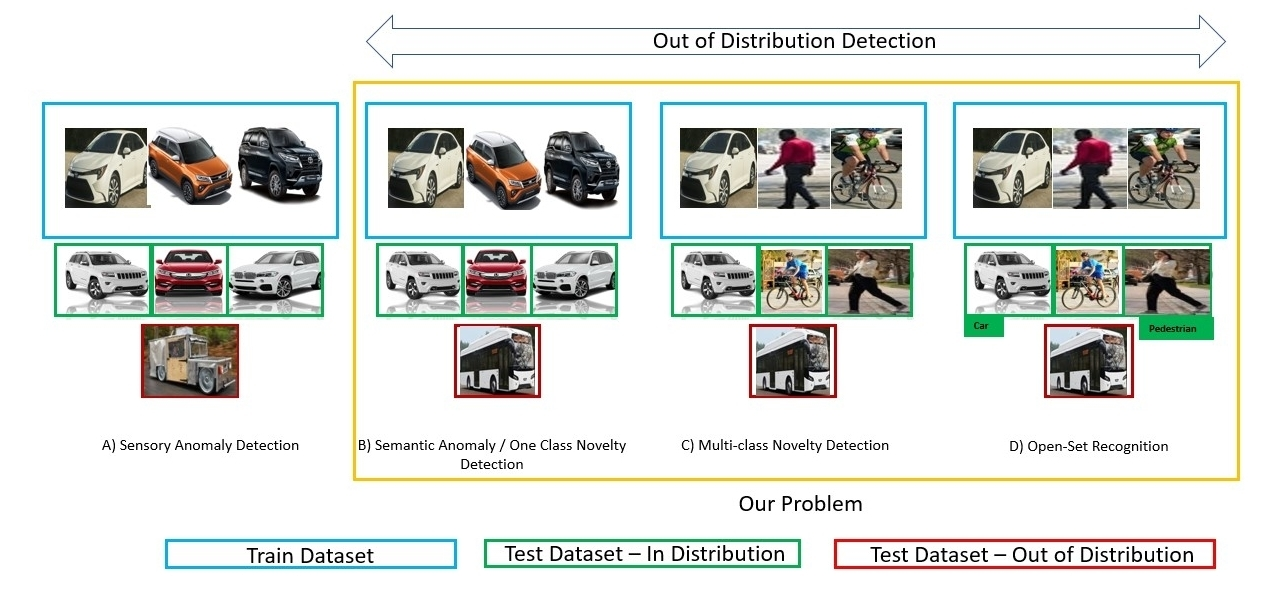
\includegraphics[scale=0.2]{images/OOD_vs_Non-OOD.jpg}
            \caption[\acrlong{ood} detection problem setting]{Class differentiation in generalized OOD detection framework}
            \label{fig:OOD_classes}
        \end{figure}
    \end{itemize}
\end{frame}

\begin{frame}{Out-of-Distribution (OOD) detection(2/3)}
    Different types of OOD data
    \begin{itemize}
        \item Data from a different domain
        \item Data with poor quality of features
        \item Data with inputs that are neither used nor prominent in the training data
    \end{itemize}
\end{frame}

\begin{frame}{Out-of-Distribution (OOD) detection(3/3)}
    Current Object Detection model performance on OOD data
    \begin{figure}[!htbp]
        \centering
      \subcaptionbox{\label{fig:1}}{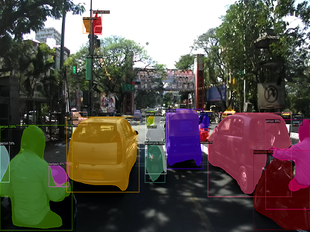
\includegraphics[scale=0.5]{images/False_Positive.png}}%\hspace{1em}
      \subcaptionbox{\label{fig:2}}{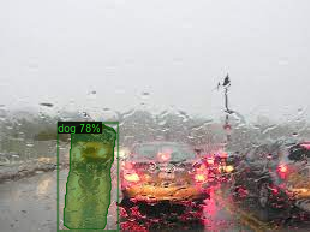
\includegraphics[scale=0.5]{images/False_Negative.png}}
      \caption[Sample False Positive and False Negative detections]{Examples of failures in object dedtection}
      \label{fig:3}
    \end{figure}
\end{frame}
\section{Solution}

\begin{frame}{OOD detector - Expectations}
    \begin{itemize}
        \item Produce a \textbf{\textit{Novelty Score (NS)}}. 
        \item NS can be a distance metric, a class-dependent probabilistic value, an entropy value, or a descriptive statistic value
        \item OOD detection can be posed as a binary classification problem.
    \end{itemize}
        
    
    
% \end{frame}

% \begin{frame}{Novelty Score - Behavior}
    
    % \begin{minipage}[t]{0.5\textwidth}
    %     $ X=
    %     \begin{cases}
    %         \text{ID}, & \text{if}\ NS \geq \delta \\
    %         \text{OOD}, & \text{otherwise} 
    %     \end{cases}
    %     $
    % \end{minipage} %%%
    % \begin{minipage}[t]{0.5\textwidth}
    %     \begin{figure}[H]
    %         \centering
    %         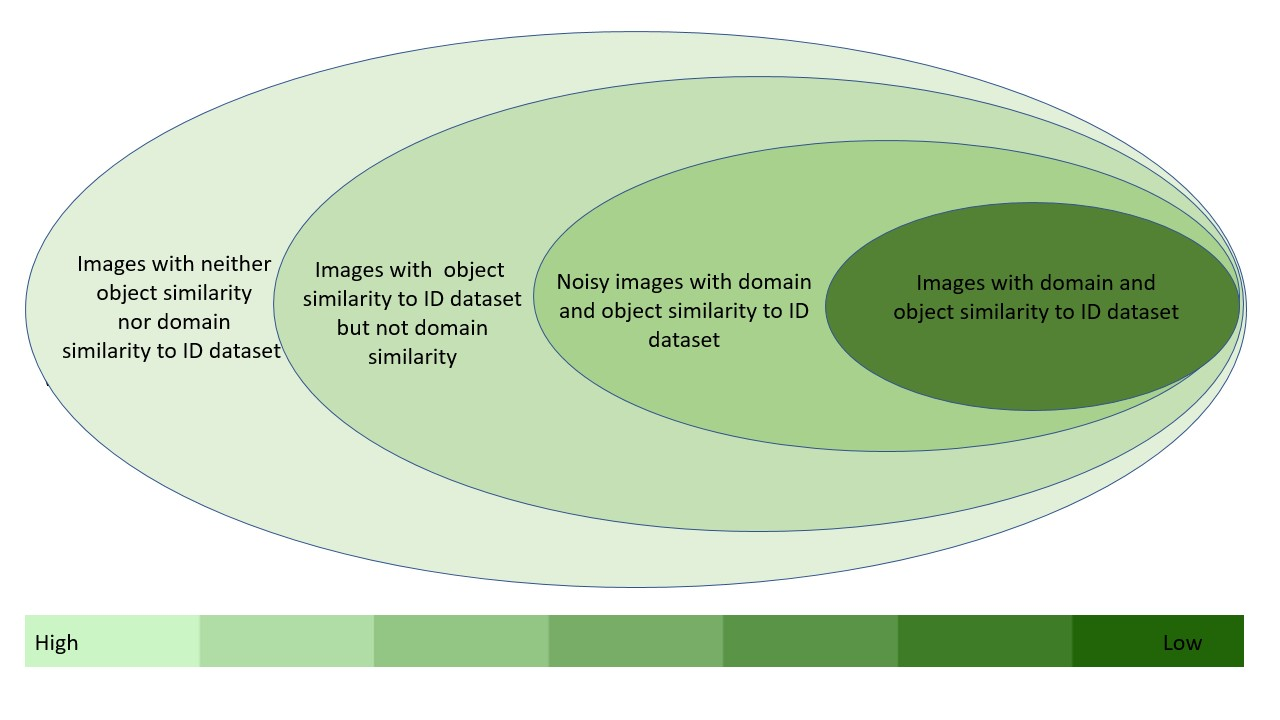
\includegraphics[scale=0.15]{images/Slide2.jpg}
    %         \caption[Novelty Score behavior]{Expected behavior of novelty score based on the nature of the OOD input}
    %         \label{fig:OD2_features}
    %     \end{figure}
    
    % \end{minipage}

    \begin{equation}
        \vcenter{\hbox{
            \begin{minipage}{7cm}
                \centering
                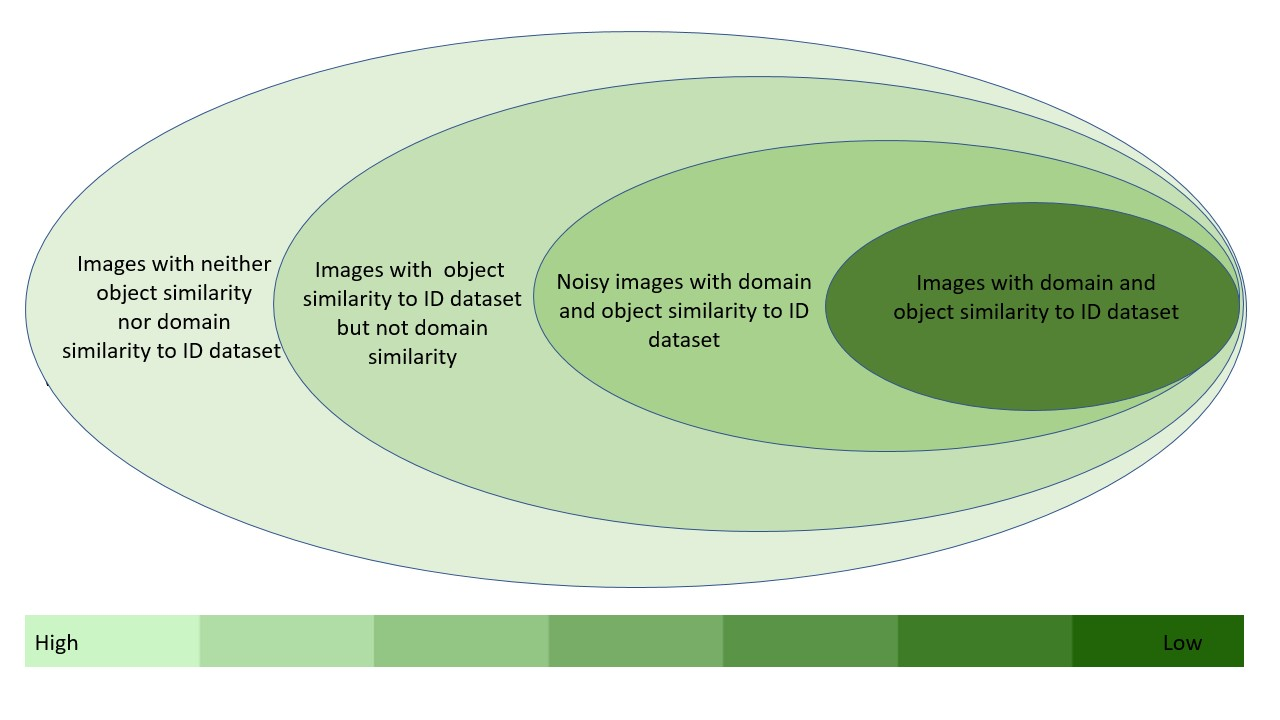
\includegraphics[scale=0.16]{images/Slide2.jpg}
                \captionof{figure}{Expected behavior of OOD detector.}
            \end{minipage}}}
        \qquad\qquad
        \begin{aligned}
            X=
                \begin{cases}
                    \text{ID}, & \text{if}\ NS \geq \delta \\
                    \text{OOD}, & \text{otherwise} 
                \end{cases}
        \end{aligned}
    \end{equation}

\end{frame}

\section{Previous works}
\begin{frame}{Previous works}
    \begin{table}[]
        \centering
        \caption{Previous works on OOD detection}
        \label{tab:my-table}
            \begin{tabular}{ll}
                \textbf{Method}             & \textbf{Works Proposed} \\ \hline
                Metric based methods        & \begin{tabular}[c]{@{}l@{}}\citet{Devries},  \citet{Oberdiek2018}, \\  \citet{Hendrycks2018} , \citet{Lee2018}\end{tabular} \\\hline
                Inconsistency based methods & \citet{liang2017enhancing} \\ \hline
                Generative methods          & \begin{tabular}[c]{@{}l@{}}\citet{Hendrycks2017},  \citet{Ren2019}, \\  \citet{VanDenOord2016}\end{tabular}    \\ \hline
                Uncertainty based methods   & \begin{tabular}[c]{@{}l@{}}\citet{Malinin2018},  \citet{Lakshminarayanan2017}, \\  \citet{VanAmersfoort2020} \\ \end{tabular}                       
            \end{tabular}
    \end{table}
    \begin{itemize}
        \item Works only for classification problem
        \item Not directly adaptable to object detection problem   
    \end{itemize}    
\end{frame}
\section{Methodology}
% \begin{frame}{Methodology}
%     In this work
%     \begin{itemize}
%         \item Proposed new benchmark dataset \textbf{Out of Distribution for Object Detection} ($OD^2$) dataset
%         \item Single-Shot Detector (SSD) is used to solve the object detection problem.
%         \item For OOD detection we decided to use
%         \begin{enumerate}
%             \item Max-Softmax score based OOD detection \citep{hendrycks17baseline}
%             \item ODIN \citep{liang2017enhancing}
%             \item Mahalanobis distance based OOD detection \citep{Lee2018}
%             \item Uncertainty based OOD detection \citep{Malinin2018, Lakshminarayanan2017}
%                 \begin{itemize}
%                     \item Bayesian Neural Network
%                     \item Sub-Ensemble
%                 \end{itemize} 
%         \end{enumerate}
%     \end{itemize}
% \end{frame}
\begin{frame}{$OD^2$ Dataset}
    \begin{table}[H]
        \centering
        \renewcommand{\arraystretch}{1.5}
        \caption{Table showing various type of images to address the OOD cases}
        \begin{adjustbox}{width=1\textwidth}
            \begin{tabular}{lllll}
            \hline
            \textbf{Purpose} & \textbf{Dataset Source} & \textbf{Classes} & \textbf{Novelty Score Behavior} & \textbf{Task} \\ \hline
            In-Distribution & BDD100K \citep{bdd100k} & \begin{tabular}[c]{@{}l@{}}Pedestrian, Rider, Car, Truck, Bus, \\ Motorcycle, Bicycle, Traffic sign\end{tabular} & Low Novelty score  & \begin{tabular}[c]{@{}l@{}}Object detector \\ performance \end{tabular} \\ \hline
            \begin{tabular}[c]{@{}l@{}}Low light and \\ bad image quality\end{tabular} & \begin{tabular}[c]{@{}l@{}}BDD100K (non-clear weather) \\ and Climate-GAN \citep{climategan} \\generated Smog images\end{tabular} & \begin{tabular}[c]{@{}l@{}}Pedestrian, Rider, Car, Truck, Bus, \\ Motorcycle, Bicycle, Traffic sign\end{tabular} & Medium Novelty Score   & Detector Robustness\\ \hline
            \begin{tabular}[c]{@{}l@{}}Classes with \\ semantic-variance\end{tabular}  & IDD \citep{Varma2019IDDAD} & Trucks, Motorcycles, Traffic Sign & High Novelty Score     & OOD detection\\ \hline
            Novel Classes  & IDD & Auto-Rickshaws  & High Novelty Score     & \begin{tabular}[c]{@{}l@{}}Multi class \\ novelty detection \end{tabular} \\ \hline
            \begin{tabular}[c]{@{}l@{}}Out-of-Domain \\ images\end{tabular} & \begin{tabular}[c]{@{}l@{}}Climate-GAN generated \\ Flood and Fire images\end{tabular} & \begin{tabular}[c]{@{}l@{}}Pedestrian, Rider, Car, Truck, Bus, \\ Motorcycle, Bicycle, Traffic sign\end{tabular} & High Novelty Score & \begin{tabular}[c]{@{}l@{}}Out-Of-Domain \\ detection \end{tabular}\\ \hline
            \end{tabular}
        \end{adjustbox}
        \label{dataset_summary}
    \end{table}
\end{frame}

\begin{frame}[allowframebreaks]{Single Shot multi-box Detector (SSD) model}
    \begin{figure}[!ht]
        \centering
        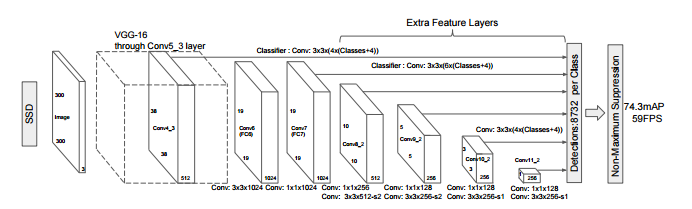
\includegraphics[scale=0.45]{images/SSD.png}
        \caption[SSD framework]{SSD framework proposed by \citet[p. 24]{Liu2016SSDSS}.}
        \label{fig:Fr-RCNN}
    \end{figure}
    \smallskip
    \begin{multicols}{2}
        \begin{itemize}
            \item Single network for detection and classification
            \item No Fully-Connected layers
            \item Low input resolution
        \end{itemize}
    \end{multicols}
% \end{frame}

% \begin{frame}{Single Shot multi-box Detector (SSD) model}
    \begin{multicols}{2} % two columns
        \begin{itemize}
            \item Default boxes
            \item Matching strategy is used,
                \begin{itemize}
                    \item $ IoU_{default box}^{ground truth}$ > 0.5
                    \item overlapped objects and simple learning 
                \end{itemize}
                
            \item Processing of features from multiple layers
                \begin{itemize}
                    \item Deep feature maps
                    \item Shallow feature maps
                \end{itemize}
        \end{itemize}

        \begin{itemize}
            \item Loss
            $$L(x, c, l, g)=\frac{1}{N}\left(L_{\text {conf }}(x, c)+\alpha L_{\text {loc }}(x, l, g)\right)$$
            \begin{itemize}
                \item $L_{conf}$ is Softmax Loss
                \item $L_{loc}$ is Smooth $L_{1}$ Loss 
            \end{itemize}
            \item Filter boxes with low confidence and NMS with 0.45 IOU
            \item Top 200 detections are considered
            
        \end{itemize}
    \end{multicols}
\end{frame}

\begin{frame}[allowframebreaks]{OOD methods}
    \begin{itemize}
        \item Max-Softmax
        
        Maximum value of softmax scores are used as novelty score
        \begin{equation}
            \setlength{\jot}{10pt}
                s\left(\mathbf{x}^{*}\right)=\max _{c} P\left(y_{c} \mid \mathbf{x}^{*} ; \mathcal{D}\right)
                \label{softmax_score}
        \end{equation}

        \item ODIN
        
        \begin{equation}
            \tilde{\boldsymbol{x}}=\boldsymbol{x}-\operatorname{esign}\left(-\nabla_{\boldsymbol{x}} \log S_{\hat{y}}(\boldsymbol{x} ; T)\right)
            \label{perturbation}
        \end{equation}

        \begin{equation}
            S_{i}(\boldsymbol{x} ; T)=\frac{\exp \left(f_{i}(\boldsymbol{x}) / T\right)}{\sum_{j=1}^{N} \exp \left(f_{j}(\boldsymbol{x}) / T\right)}
            \label{ODIN_Softmaxscore}
        \end{equation}

        \begin{itemize}
            \item $\epsilon$ is the perturbation magnitude
            \item $T$ is the Temperature
        \end{itemize}
        
        \newpage
        
        \item Mahalanobis distance based OOD detection
        
        assuming intermediate layer features follow class-conditional Gaussian distributions with tied covariances

        % \begin{equation}
        %     M(x)=\max _{c}-\left(f(x)-\hat{\mu}_{c}\right)^{T} \hat{\Sigma}^{-1}\left(f(x)-\hat{\mu}_{c}\right), where. \\
        %     & \hat{\mu}_{c}=\frac{1}{N_{c}} \sum_{i: y_{c}=c} f\left(x_{i}\right) \\
        %     & \hat{\Sigma}=\frac{1}{N} \sum_{c} \sum_{i: y_{c}=c}\left(f\left(x_{i}\right)-\hat{\mu}_{c}\right)\left(f\left(x_{i}\right)-\hat{\mu}_{c}\right)^{T} \\
        % \end{equation}

        \begin{equation}
            M(x)=\max _{c}-\left(f(x)-\hat{\mu}_{c}\right)^{T} \hat{\Sigma}^{-1}\left(f(x)-\hat{\mu}_{c}\right)
        \end{equation}

        $$\hat{\mu}_{c}=\frac{1}{N_{c}} \sum_{i: y_{c}=c} f\left(x_{i}\right)$$
            
        $$\hat{\Sigma}=\frac{1}{N} \sum_{c} \sum_{i: y_{c}=c}\left(f\left(x_{i}\right)-\hat{\mu}_{c}\right)\left(f\left(x_{i}\right)-\hat{\mu}_{c}\right)^{T} $$ \newline \newline \newline
        
        \item Uncertainty based OOD detection
        
            \begin{itemize}
                \item quantifies trustworthiness in the model output
                \begin{itemize}
                        \item<.-> epistemic uncertainty, higher in areas of low data density.
                        \item<.-> aleatoric uncertainty, labelling and measurement noise
                \end{itemize}
                \item OOD data is implicitly modeled by epistemic uncertainty
                \item To quantify epistemic uncertainty, we used
                \begin{itemize}
                    \item<.-> Bayesian Neural Netowrk.
                    \item<.-> Deep Sub-Ensembles
                \end{itemize}
            \end{itemize}
            \pagebreak
        \begin{itemize}
            \item Bayesian Neural Network
            \begin{columns}
                \column{0.38\linewidth}
                %    \centering
                   \begin{figure}
                        \centering
                        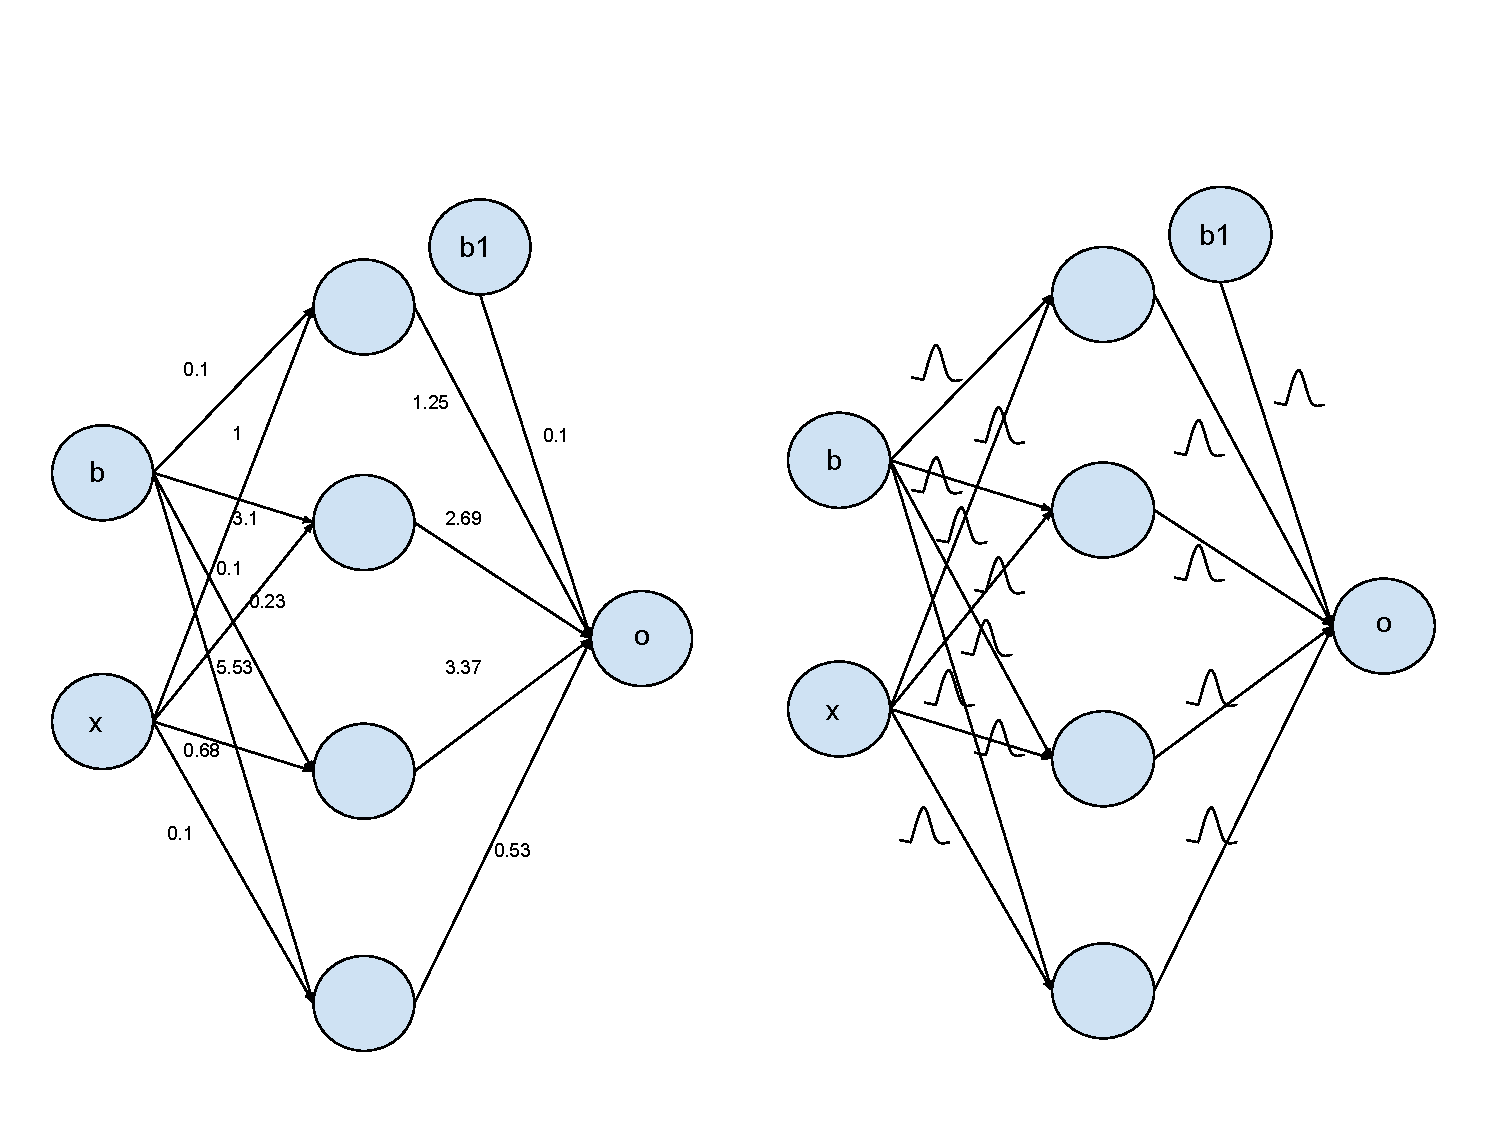
\includegraphics[scale=0.275]{images/BNN.pdf}
                        \caption{Bayesian Neural Network}
                   \end{figure}
                   
                %    \caption{Bayesian Neural Netowrk}
                 \column{0.38\linewidth}
                    \begin{itemize}
                        \item Bayesian Flipout layers \citep{Wen2018}
                        \item Reparameterization trick for training \citep{Kingma2015}
                        \item Prior $P(w)$ $\sim$ $N(0, 1)$
                        \item multiple forward passes for uncertainty quantification \newline \newline
                    \end{itemize}
            \end{columns} 
            \pagebreak
            \item Sub-Ensemble Network 
            \begin{columns}
                \column{0.38\linewidth}
                    \begin{figure}
                        % \centering
                        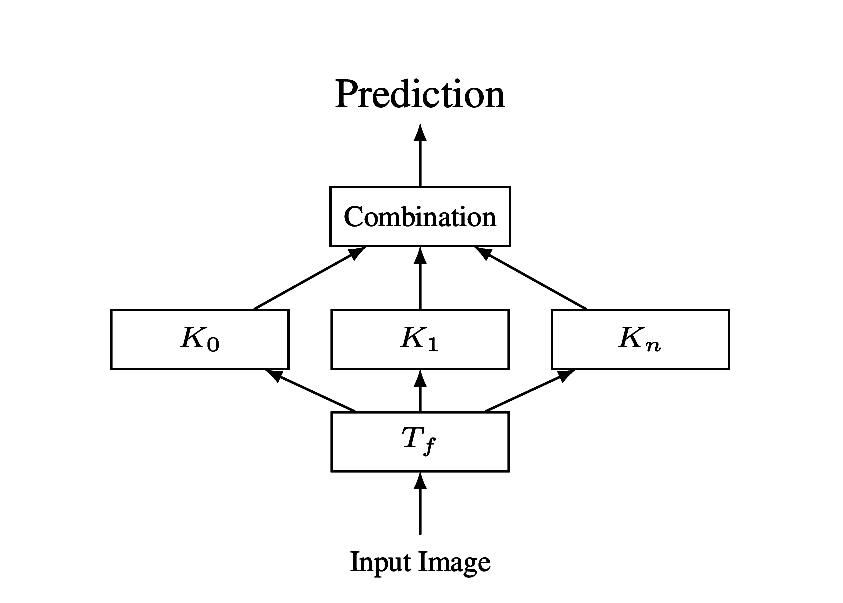
\includegraphics[scale=0.275]{images/subensembles.png}
                        \caption{Sub-Ensemble Network}
                    \end{figure}
                 \column{0.38\linewidth}
                    \begin{itemize}
                        \item Model is divided into Trunk and Task layers
                        \item Trunk layers has best performing weights restored and cannot be trained
                        \item Task layers are randomly initialized and re-trained
                        \item Random initialization of layers creates ensemble model. 
                    \end{itemize}
            \end{columns} \newpage
            \item Novelty Score \newline
            
            Entropy
            \begin{equation}
                \label{Entropy}
                \begin{array}{l}
                    \text{Entropy} =-\sum_{i=1}^{C} P\left(c_i \mid \mathbf{x}^{*} ; \mathcal{D}\right) \ln P\left(c_i \mid \mathbf{x}^{*} ; \mathcal{D}\right) 
                \end{array}
            \end{equation} \newline

            Box deviation is the square root of the trace of the covariance matrix $C(x^{*})$.
            \begin{equation}
                C\left(\mathbf{x}^{*}\right)=\frac{1}{N} \sum_{i=1}^{N} \hat{\mathbf{v}}_{\mathbf{x}^{*}}^{i} \hat{\mathbf{v}}_{\mathbf{x}^{*}}^{i^{T}}-\mathbf{I}_{\mathbf{x}^{*}} \mathbf{I}_{\mathbf{x}^{*}}^{T}
            \end{equation}

        \end{itemize}
    \end{itemize}
\end{frame}

\section{Results}
\begin{frame}[allowframebreaks]{SSD Object Detection Results}
    %\resizebox{\linewidth}{!}{
    %}

    \begin{columns}
        \column{0.38\linewidth}
            \begin{table}
                \caption{AP values for various classes using vanilla-SSD Prior boxes}
                \begin{tabular}{ll}
                    \hline
                        \textbf{Class} & \textbf{score} \\ \hline
                        Pedestrian     & 0.006              \\ \hline
                        Rider          & 0.004              \\ \hline
                        Car            & 0.095              \\ \hline
                        Truck          & 0.083              \\ \hline
                        Bus            & 0.15               \\ \hline 
                        Motorcycle     & 0.045              \\ \hline
                        Bicycle        & 0.092              \\ \hline
                        Traffic Sign   & 0.001              \\ \hline
                        \textbf{Mean}  & 0.059  \\\hline
                \end{tabular}
            \end{table}
        \column{0.5\linewidth}
            \begin{figure}[!ht]
                \centering
                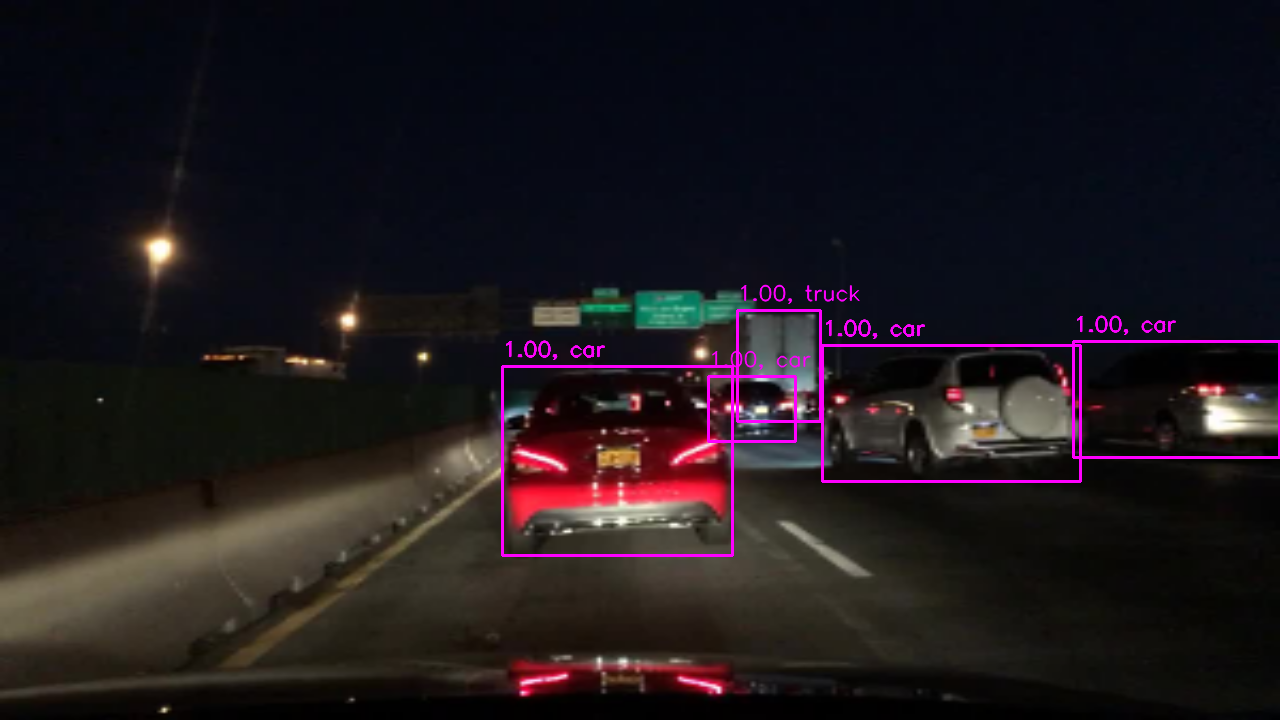
\includegraphics[scale=0.175]{images/9.png}
                \caption[SSD framework]{Positively matched vanilla prior boxes with ground truth boxes.}
            \end{figure}
    \end{columns}

    \begin{itemize}
        \item Poor performance, can be improved by tuning
    \end{itemize}

    \begin{columns}
        \column{0.38\linewidth}
            \begin{table}
                \caption{AP values for various classes using tuned Prior boxes}
                \begin{tabular}{ll}
                    \hline
                        \textbf{Class} & \textbf{score} \\ \hline
                        Pedestrian     & 0.165              \\ \hline
                        Rider          & 0.135              \\ \hline
                        Car            & 0.479              \\ \hline
                        Truck          & 0.389              \\ \hline
                        Bus            & 0.389               \\ \hline 
                        Motorcycle     & 0.163              \\ \hline
                        Bicycle        & 0.213              \\ \hline
                        Traffic Sign   & 0.186              \\ \hline
                        \textbf{Mean}  & 0.265  \\\hline
                \end{tabular}
            \end{table}
        \column{0.5\linewidth}
            \begin{figure}[!ht]
                \centering
                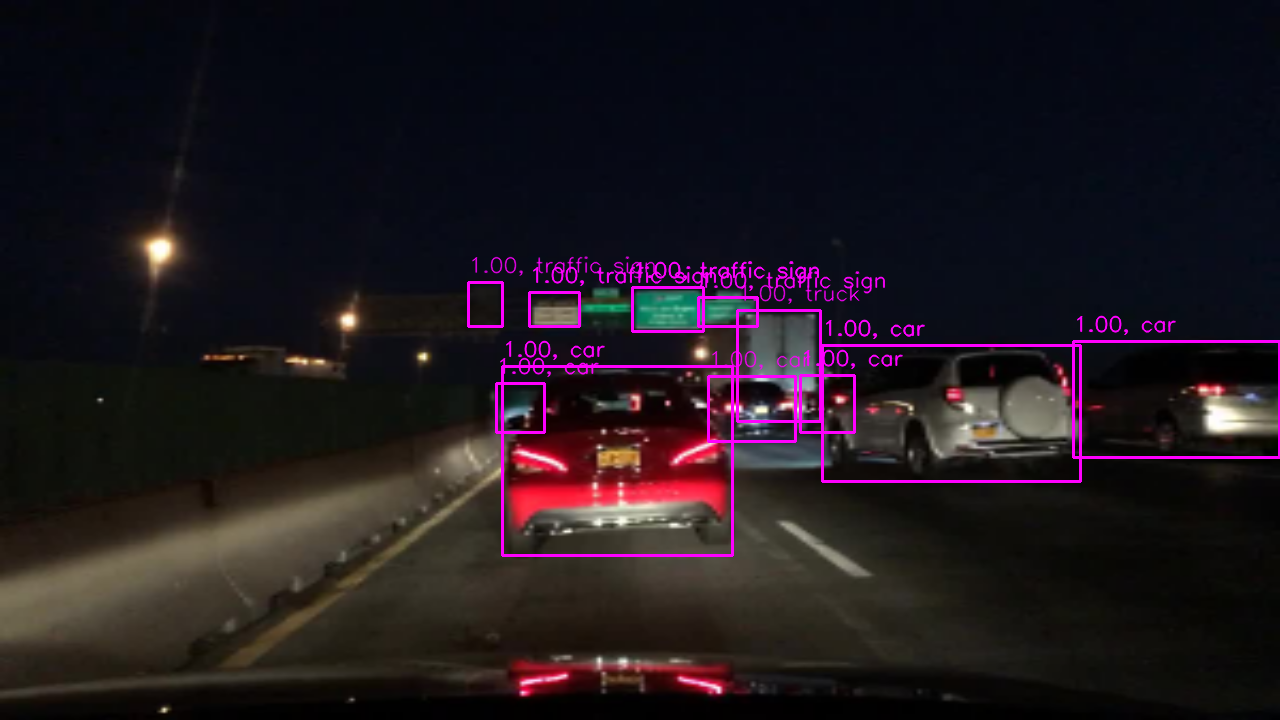
\includegraphics[scale=0.175]{images/tuned_9.png}
                \caption[SSD framework]{Positively matched tuned prior boxes with ground truth boxes..}
            \end{figure}
    \end{columns}
    \begin{itemize}
        \item improved performance
    \end{itemize}
\end{frame}

\begin{frame}{OOD Detection - MaxSoftmax}
    \begin{columns}
        \column{0.38\linewidth}
            \begin{itemize}
                \item ROC score of 48 \%
                \item poorer than un-biased random classifier
                \item complex scenarios, class overlap
            \end{itemize}
        \column{0.5\linewidth}
            \begin{figure}[!ht]
                \centering
                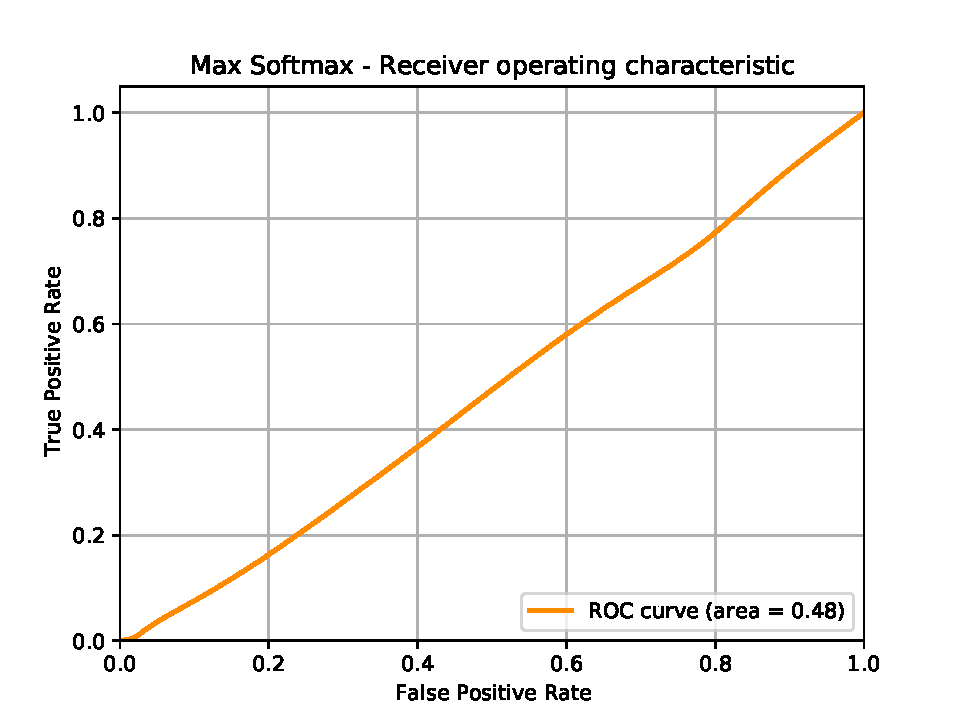
\includegraphics[scale=0.45]{images/Max Softmax_ROC.pdf}
                \caption[SSD framework]{AUROC curve for OOD detection using softmax scores.}
            \end{figure}
    \end{columns}
\end{frame}

\begin{frame}[allowframebreaks]{OOD Detection - ODIN}
    \begin{itemize}
        \item gradient of loss w.r.t input image is calculated and scaled by a perturbation magnitude. 
        \item input image is modified by subtracting the perturbation.
    \end{itemize}
    \begin{columns}[c]
        % create the column with the first image, that occupies
        % half of the slide
            \begin{column}{.33\textwidth}
            \begin{figure}
                \centering
                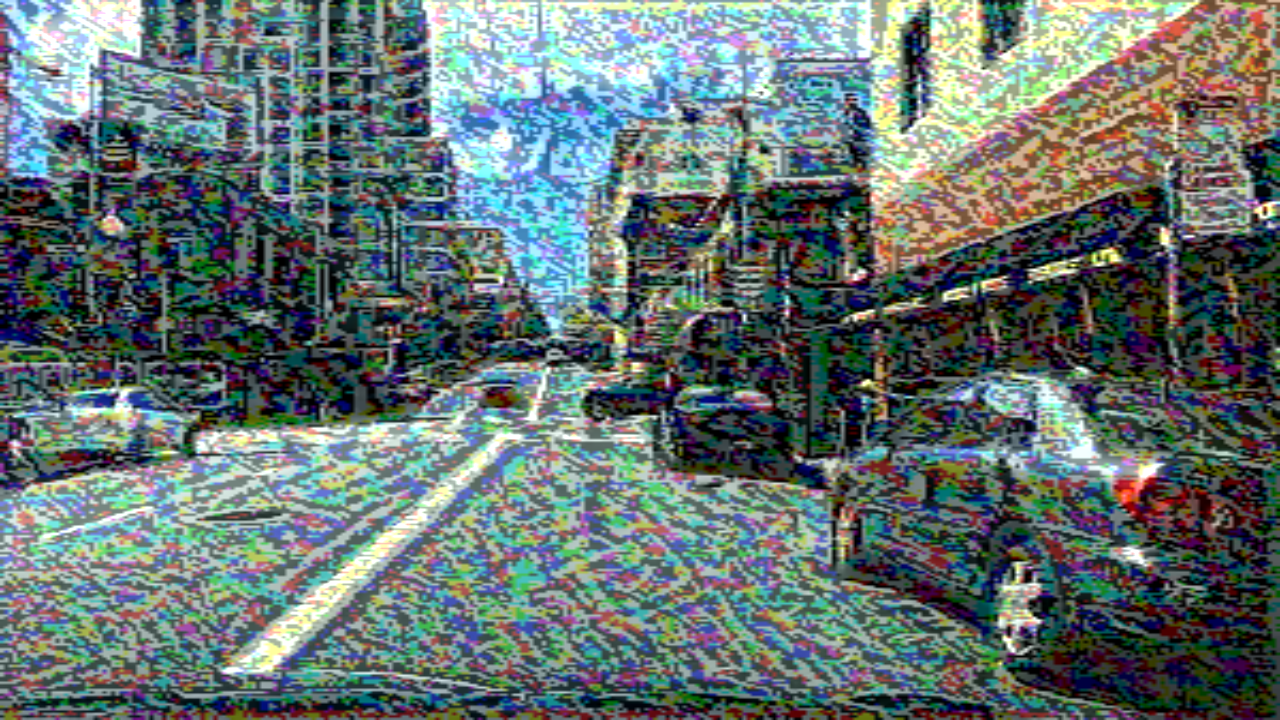
\includegraphics[width=0.9\textwidth]{images/image_0.2_10.png}
                \caption{magnitude=0.2, Temperature=10}
            \end{figure}      
            \end{column}
        % create the column with the second image, that also
        % occupies half of the slide
            \begin{column}{.33\textwidth}
            \begin{figure}
                \centering
                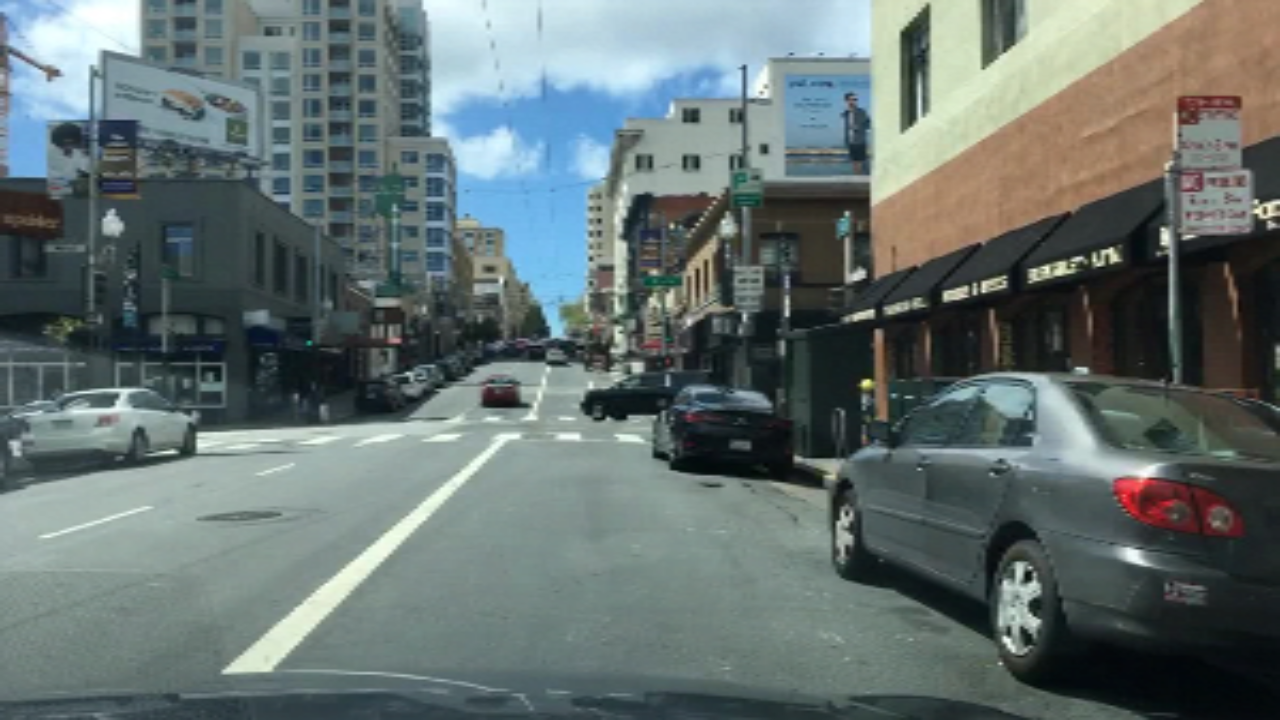
\includegraphics[width=0.9\textwidth]{images/image_0.005_1000.png}
                \caption{magnitude=0.005, Temperature=100}
            \end{figure}
            \end{column}

            \begin{column}{.33\textwidth}
                \begin{figure}
                    \centering
                    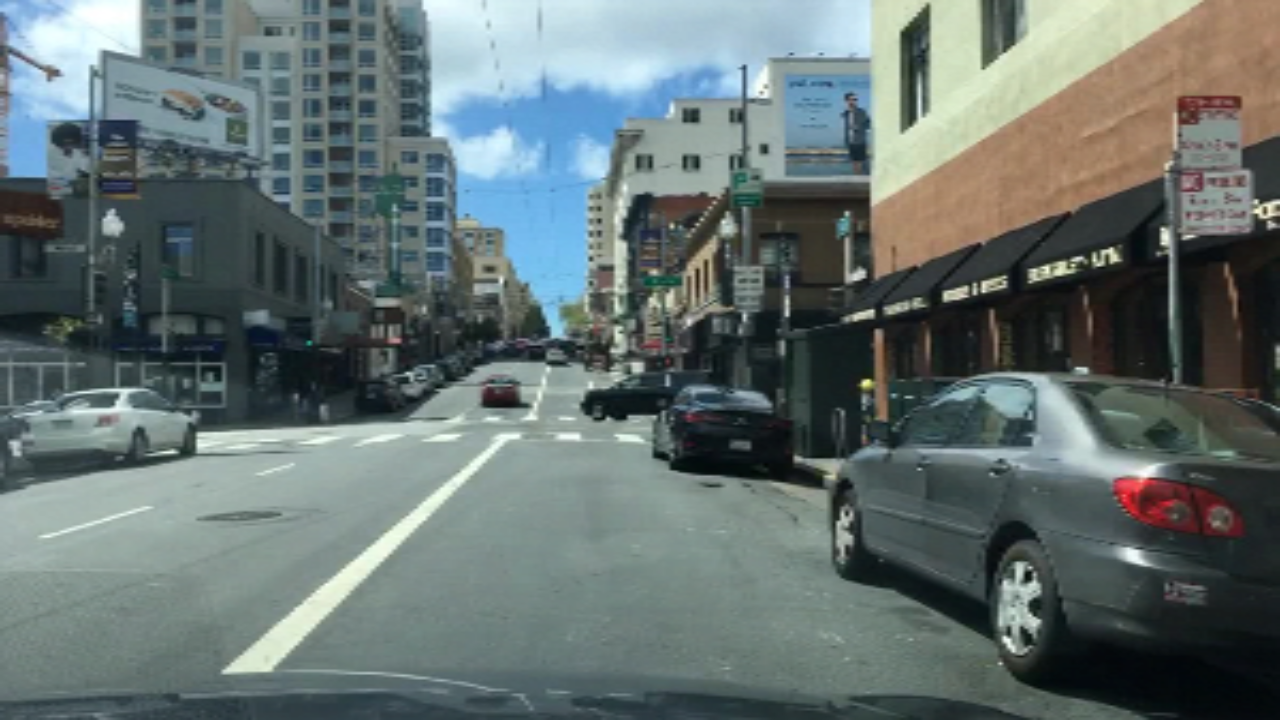
\includegraphics[width=0.9\textwidth]{images/image_0.005_10.png}
                    \caption{magnitude=0.005, Temperature=10}
                \end{figure}
                \end{column}
        \end{columns}

        \begin{itemize}
            \item hyperparameters are tuned using a fraction of test images sampled from IDD dataset
            \item Perturbation Magnitude 0.2 and Temperature of 1000
        \end{itemize}

        \framebreak

        \begin{columns}
            \column{0.38\linewidth}
                \begin{itemize}
                    \item ROC score of 54 \%
                    \item improvement over max-softmax method 
                    \item effect of perturbation is not observed in smaller objects
                \end{itemize}
            \column{0.5\linewidth}
                \begin{figure}[!ht]
                    \centering
                    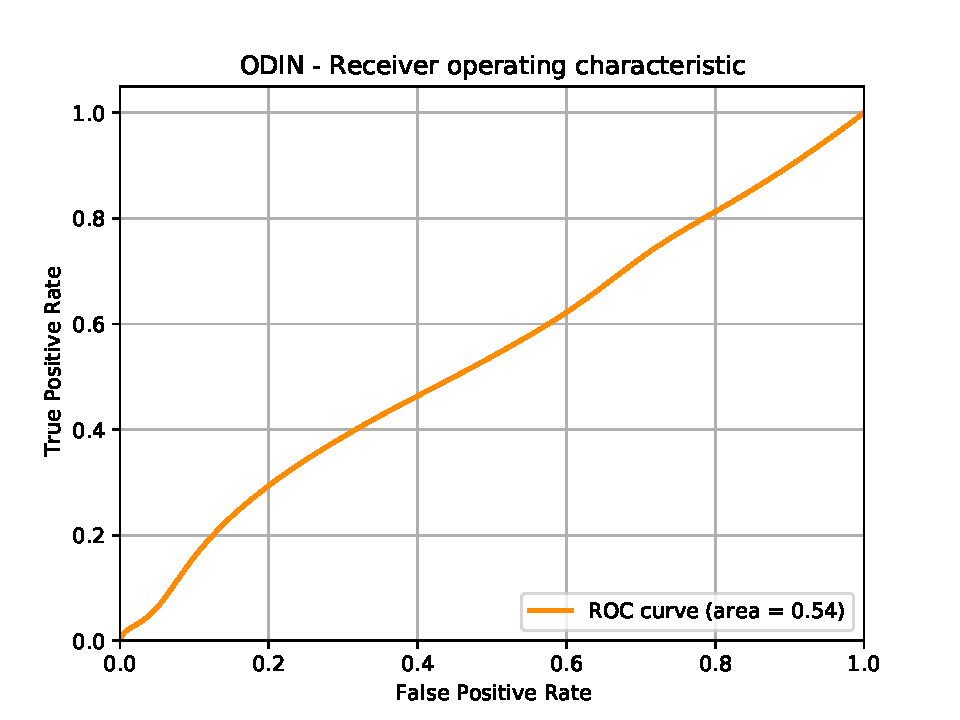
\includegraphics[scale=0.45]{images/BDD100K vs IDD_ODIN_ROC.pdf}
                    \caption[SSD framework]{AUROC curve for OOD detection using softmax scores after applying ODIN}
                \end{figure}
        \end{columns}
\end{frame}

\begin{frame}[allowframebreaks]{OOD Detection - Mahalanobis distance}
    \begin{itemize}
        \item class-wise mean vectors of each class and a tied covariance matrix using the features from the penultimate layer
        \item images with other classes masked out by the mean of the image
    \end{itemize}
    \begin{columns}
        \column{0.38\linewidth}
            \begin{itemize}
                \item flattened penultimate layer of SSD is of shape (78588 × 1)
                \item the covariance matrix is of shape (78588 × 78588)
                \item calculating it is not possible with
                available resources.
            \end{itemize}
        \column{0.5\linewidth}
            \begin{figure}[!ht]
                \centering
                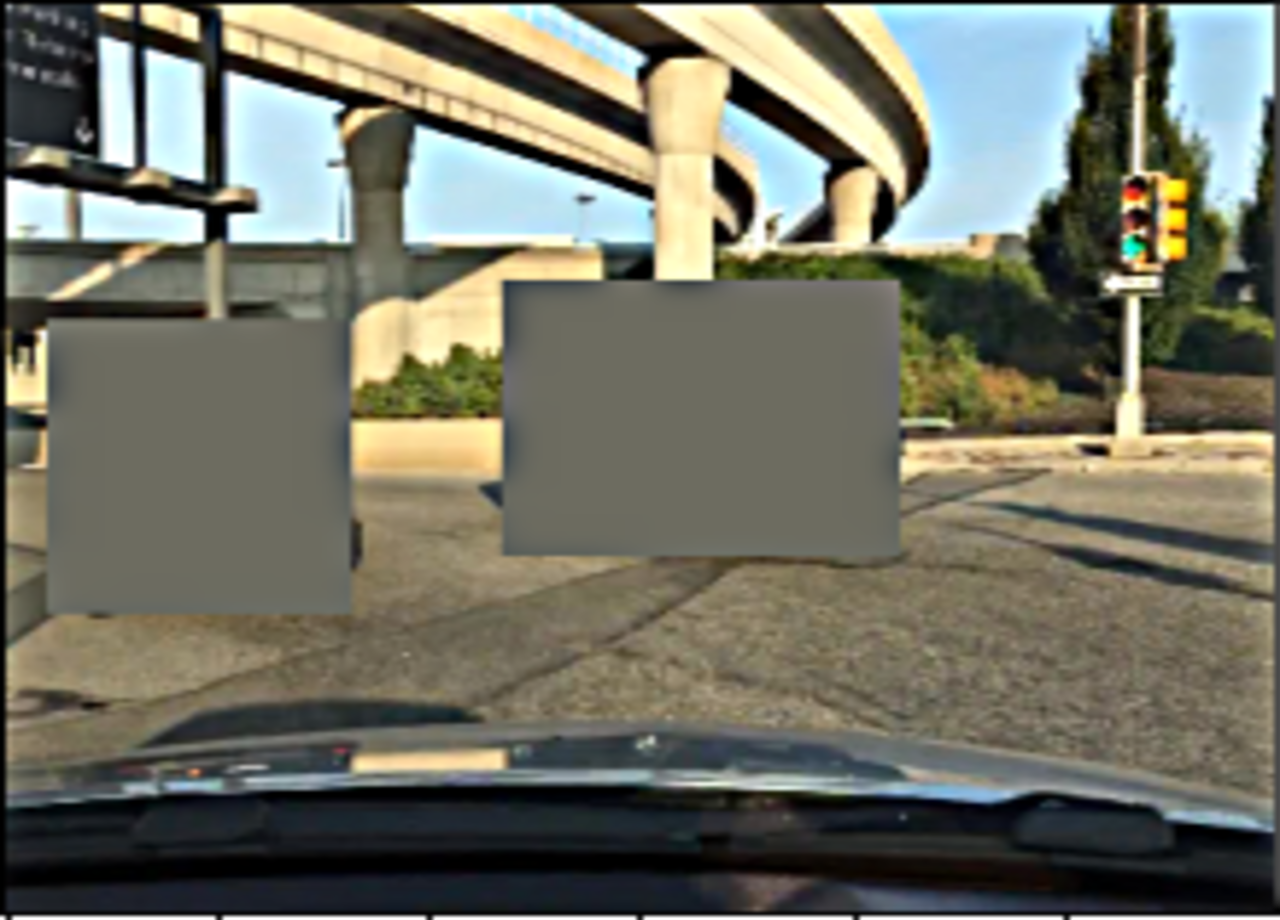
\includegraphics[scale=0.125]{images/rsz_1classspecific-image.png}
                \caption[SSD framework]{Class masked images to extract class specific mean and variance}
            \end{figure}
    \end{columns}
\end{frame}

\begin{frame}[allowframebreaks]{UQ models - Performance}
    \begin{columns}
        \column{0.38\linewidth}
            Layers highlights in green are chosen as 
            \begin{itemize}
                \setlength\itemsep{1em}
                \item Flipout layers to model Bayesian-SSD
                \item Task network to model Sub-Ensemble SSD
            \end{itemize} 
        \column{0.5\linewidth}
            \begin{figure}
                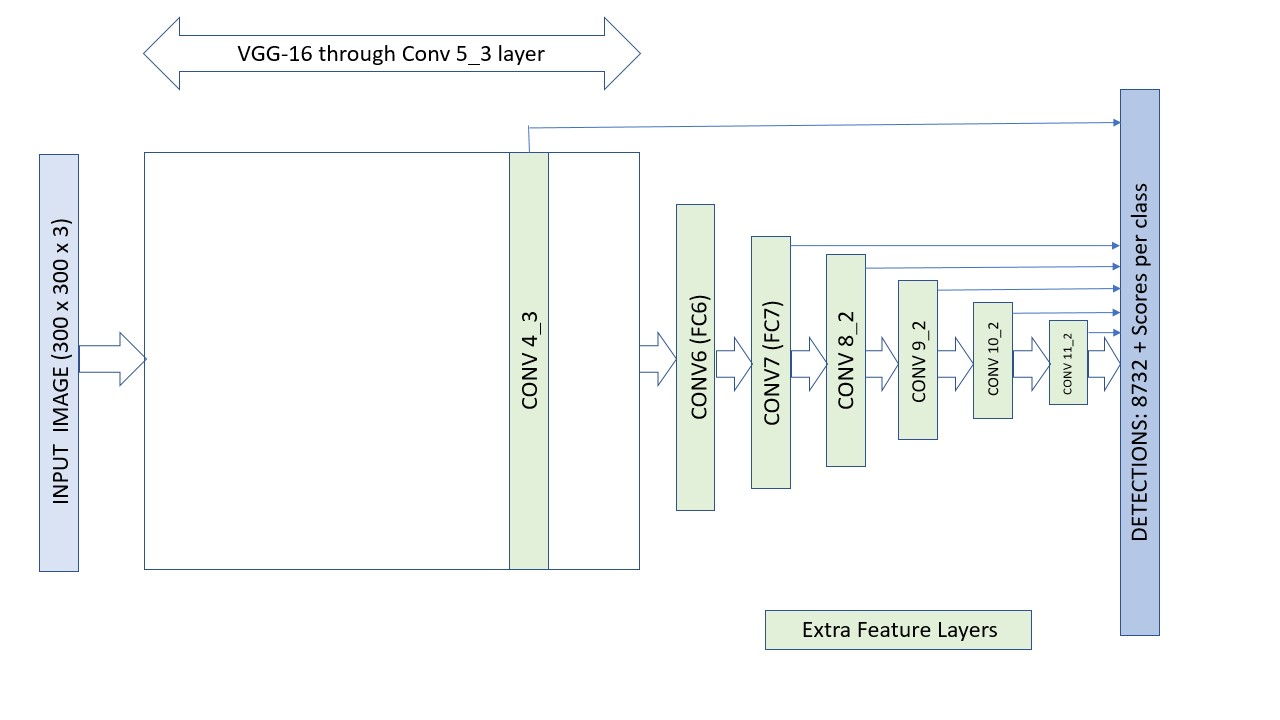
\includegraphics[scale=0.25]{images/SSD300_flipout.jpg}
                \caption{modified SSD for uncertainty quantification}
            \end{figure}
    \end{columns}
    \pagebreak
    \begin{itemize}
        \begin{columns}
            \column{0.5\linewidth}
            \item Bayesian SSD model
                \begin{table}
                    \caption{AP values for various classes using tuned Prior boxes}
                    \begin{tabular}{ll}
                        \hline
                            \textbf{Class} & \textbf{score} \\ \hline
                            Pedestrian     & 0.172            \\ \hline
                            Rider          & 0.149              \\ \hline
                            Car            & 0.476              \\ \hline
                            Truck          & 0.4              \\ \hline
                            Bus            & 0.401               \\ \hline 
                            Motorcycle     & 0.196              \\ \hline
                            Bicycle        & 0.232              \\ \hline
                            Traffic Sign   & 0.184              \\ \hline
                            \textbf{Mean}  & 0.276  \\\hline
                    \end{tabular}
                \end{table}
            \column{0.5\linewidth}
            \item Sub-Ensemble SSD model
            \begin{table}
                \caption{AP values for various classes using tuned Prior boxes}
                \begin{tabular}{ll}
                    \hline
                        \textbf{Class} & \textbf{score} \\ \hline
                        Pedestrian     & 0.167          \\ \hline
                        Rider          & 0.144              \\ \hline
                        Car            & 0.47              \\ \hline
                        Truck          & 0.393             \\ \hline
                        Bus            & 0.396               \\ \hline 
                        Motorcycle     & 0.181              \\ \hline
                        Bicycle        & 0.211              \\ \hline
                        Traffic Sign   & 0.171              \\ \hline
                        \textbf{Mean}  & 0.267  \\\hline
                \end{tabular}
            \end{table}
        \end{columns}
    \end{itemize}

    \begin{figure}[H]
        \captionsetup[table]{skip=0pt}
           \centering
       % \end{figure}
       % \begin{figure}[H] \ContinuedFloat
           \begin{subfigure}[t]{0.495\textwidth}
               \centering
               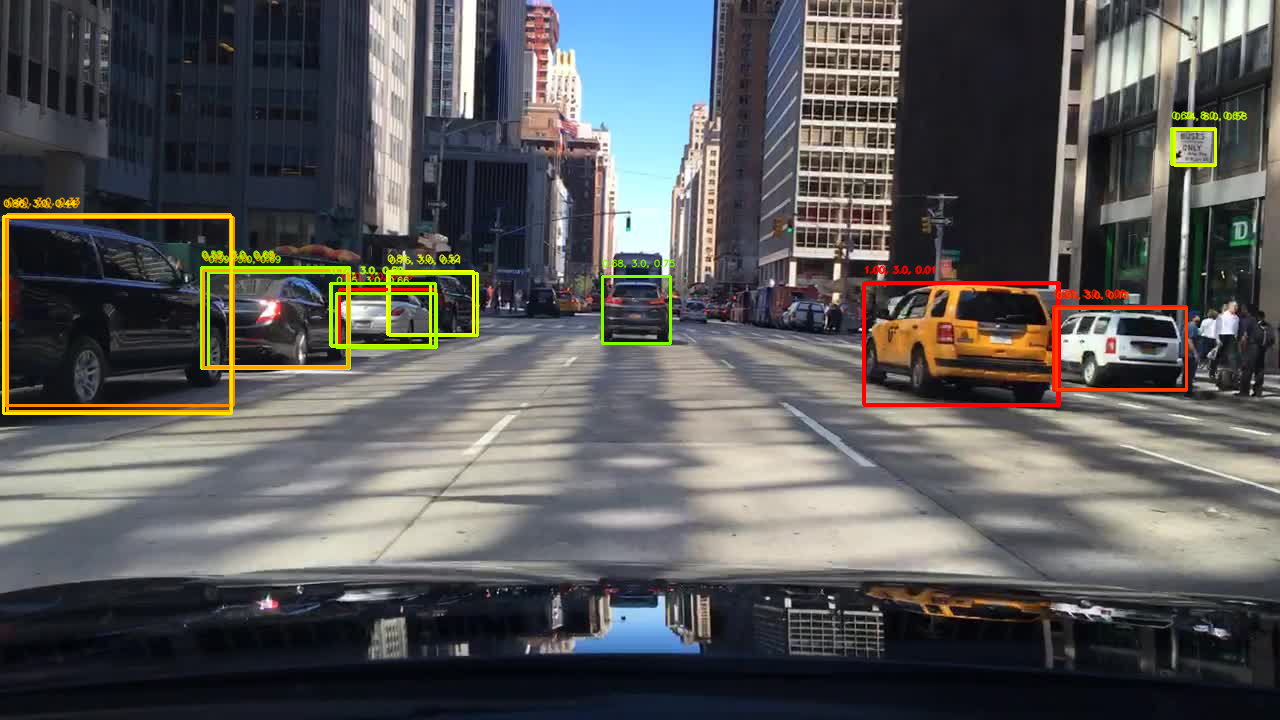
\includegraphics[width=\textwidth]{images/det_images/bdd_bnn_variances_1.png}
               \caption{Detections with variances represented as ellipses}
           \end{subfigure}
           %
           \begin{subfigure}[t]{0.495\textwidth}
               \centering
               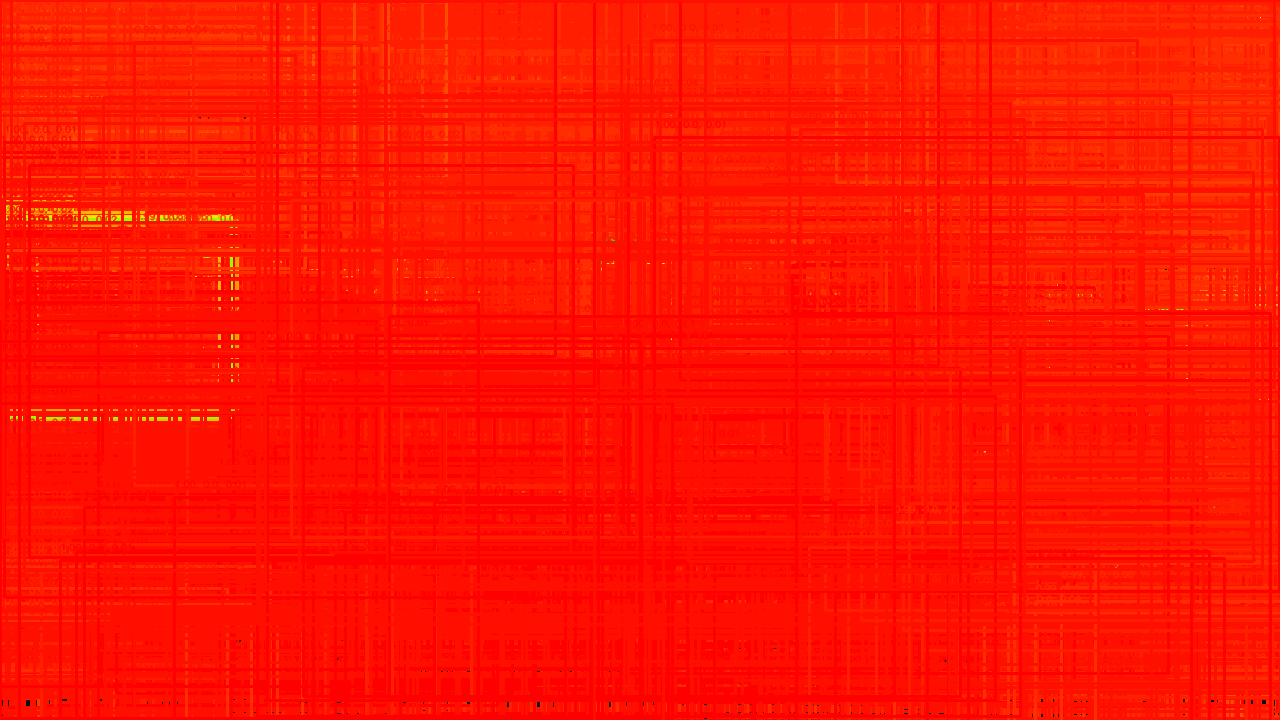
\includegraphics[width=\textwidth]{images/det_images/all_bnn_bdd_1.png}
               \caption{Visualizing all 8732 boxes regressed by SSD300}
           \end{subfigure}
           
           \begin{center}
               \begin{subfigure}[t]{0.275\textwidth}
               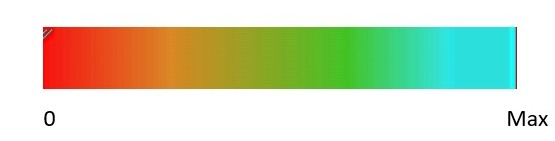
\includegraphics[width=\textwidth]{images/Slide4.jpg}
               \caption{Colormap}
           \end{subfigure}
           \end{center}
           \caption{Inference of Bayesian-SSD300 model on a sample image from BDD}
       \end{figure}
    
       \begin{figure}[H]
        \captionsetup[table]{skip=0pt}
           \centering
       % \end{figure}
       % \begin{figure}[H] \ContinuedFloat
           \begin{subfigure}[t]{0.495\textwidth}
               \centering
               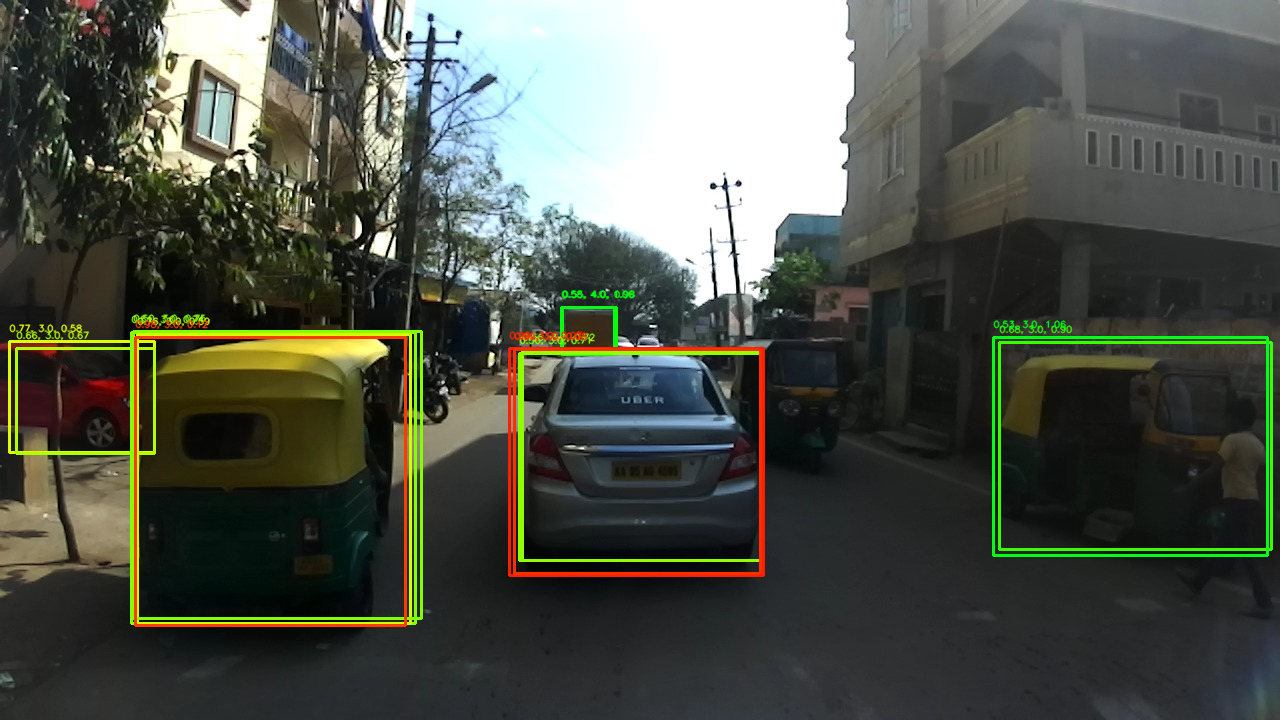
\includegraphics[width=\textwidth]{images/det_images/idd_bnn_variances_1.png}
               \caption{Detections with variances represented as ellipses}
           \end{subfigure}
           %
           \begin{subfigure}[t]{0.495\textwidth}
               \centering
               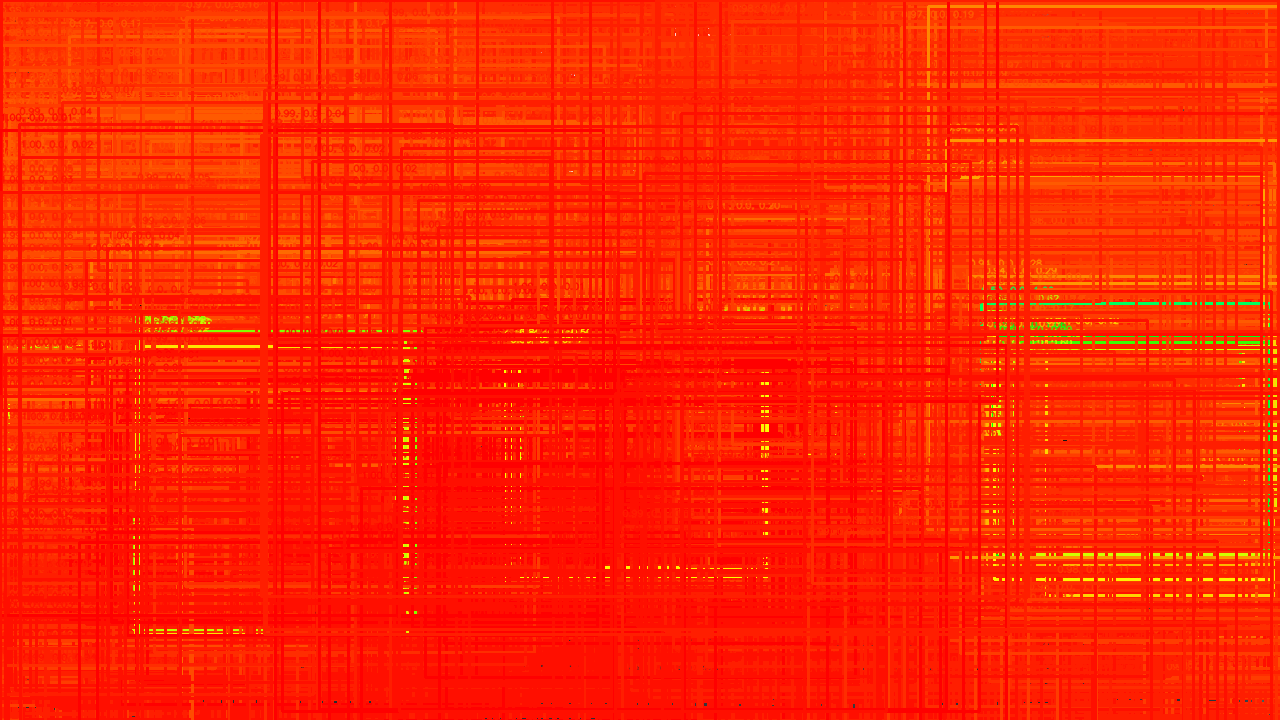
\includegraphics[width=\textwidth]{images/det_images/all_bnn_idd_1.png}
               \caption{Visualizing all 8732 boxes regressed by SSD300}
           \end{subfigure}
           \caption{Inference of Bayesian-SSD300 model on a sample image from BDD}
       \end{figure}

       \begin{figure}[H]
        \captionsetup[table]{skip=0pt}
           \centering
       % \end{figure}
       % \begin{figure}[H] \ContinuedFloat
           \begin{subfigure}[t]{0.495\textwidth}
               \centering
               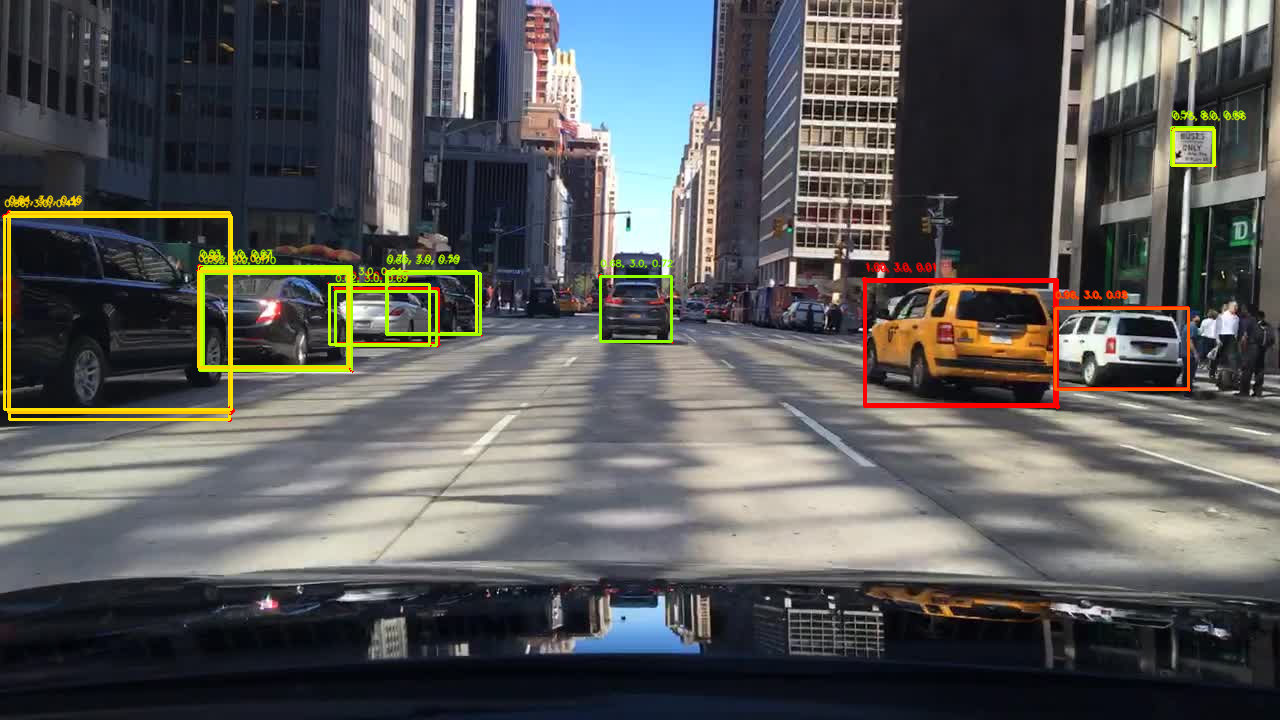
\includegraphics[width=\textwidth]{images/det_images/bdd_subens_entropies_0.png}
               \caption{Detections with variances represented as ellipses}
           \end{subfigure}
           %
           \begin{subfigure}[t]{0.495\textwidth}
               \centering
               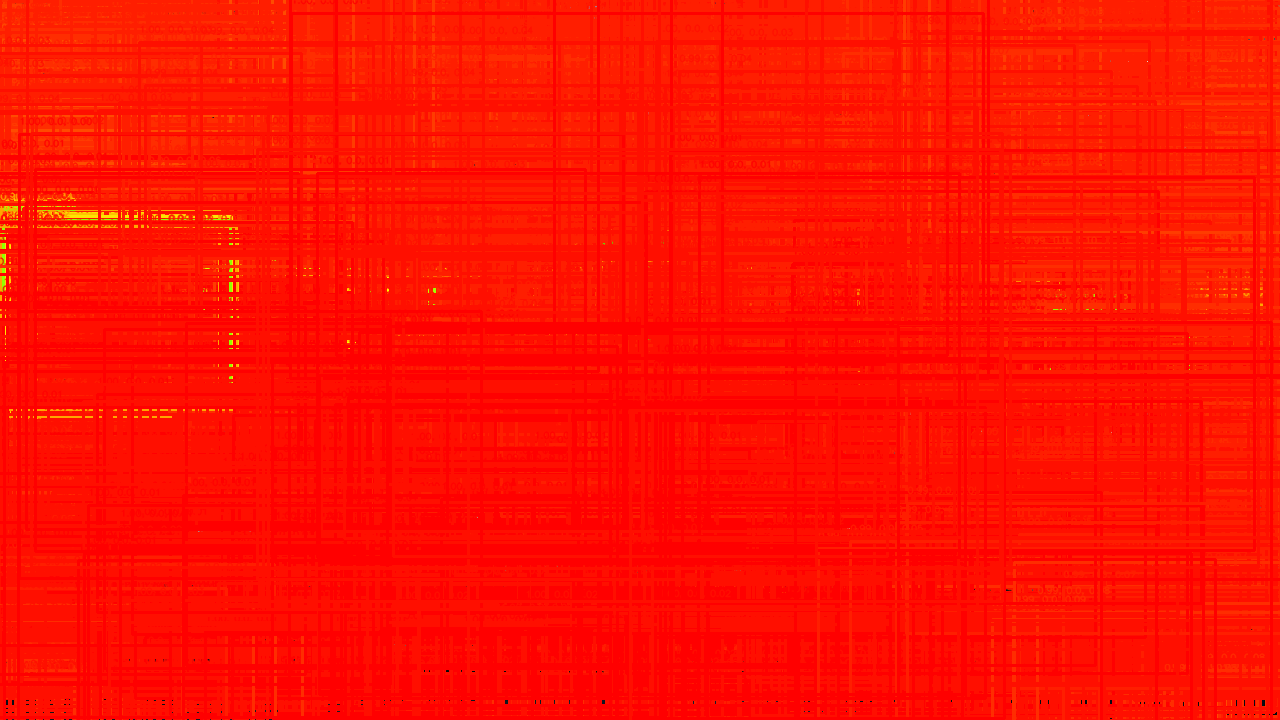
\includegraphics[width=\textwidth]{images/det_images/all_subens_bdd_1.png}
               \caption{Visualizing all 8732 boxes regressed by SSD300}
           \end{subfigure}
           \caption{Inference of Bayesian-SSD300 model on a sample image from BDD}
       \end{figure}
    
       \begin{figure}[H]
        \captionsetup[table]{skip=0pt}
           \centering
       % \end{figure}
       % \begin{figure}[H] \ContinuedFloat
           \begin{subfigure}[t]{0.495\textwidth}
               \centering
               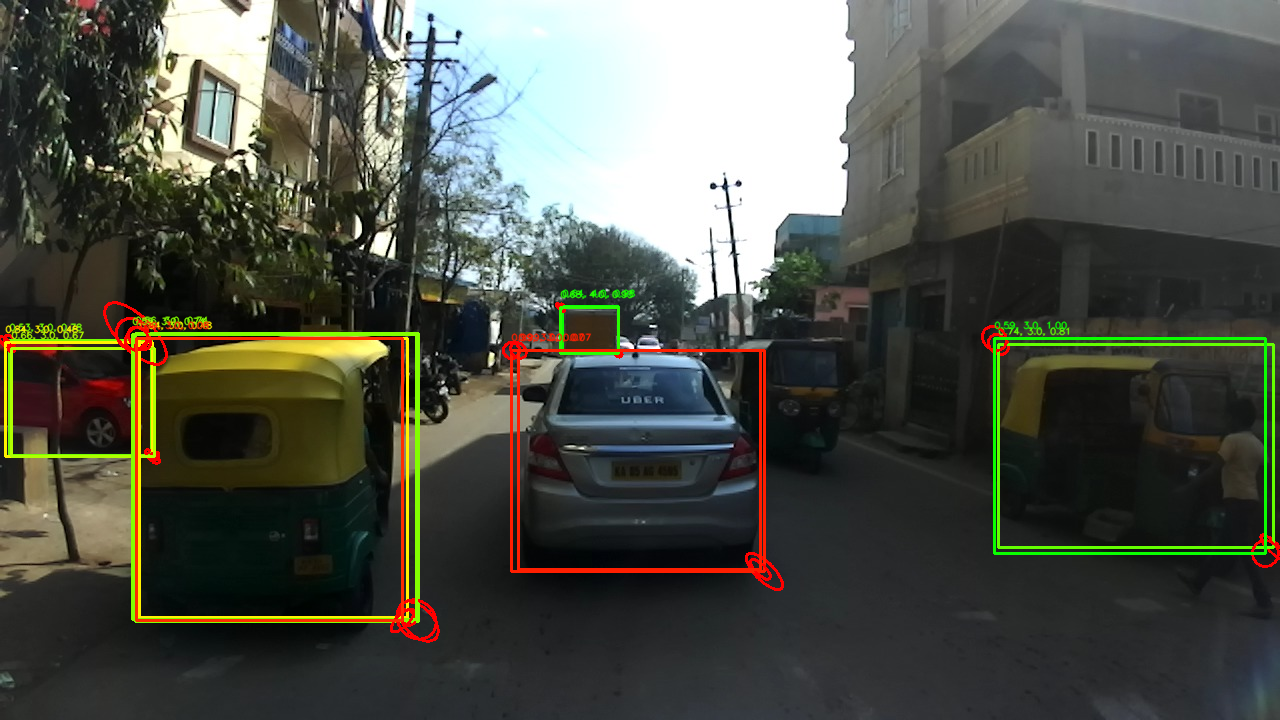
\includegraphics[width=\textwidth]{images/det_images/idd_subens_variances_1.png}
               \caption{Detections with variances represented as ellipses}
           \end{subfigure}
           %
           \begin{subfigure}[t]{0.495\textwidth}
               \centering
               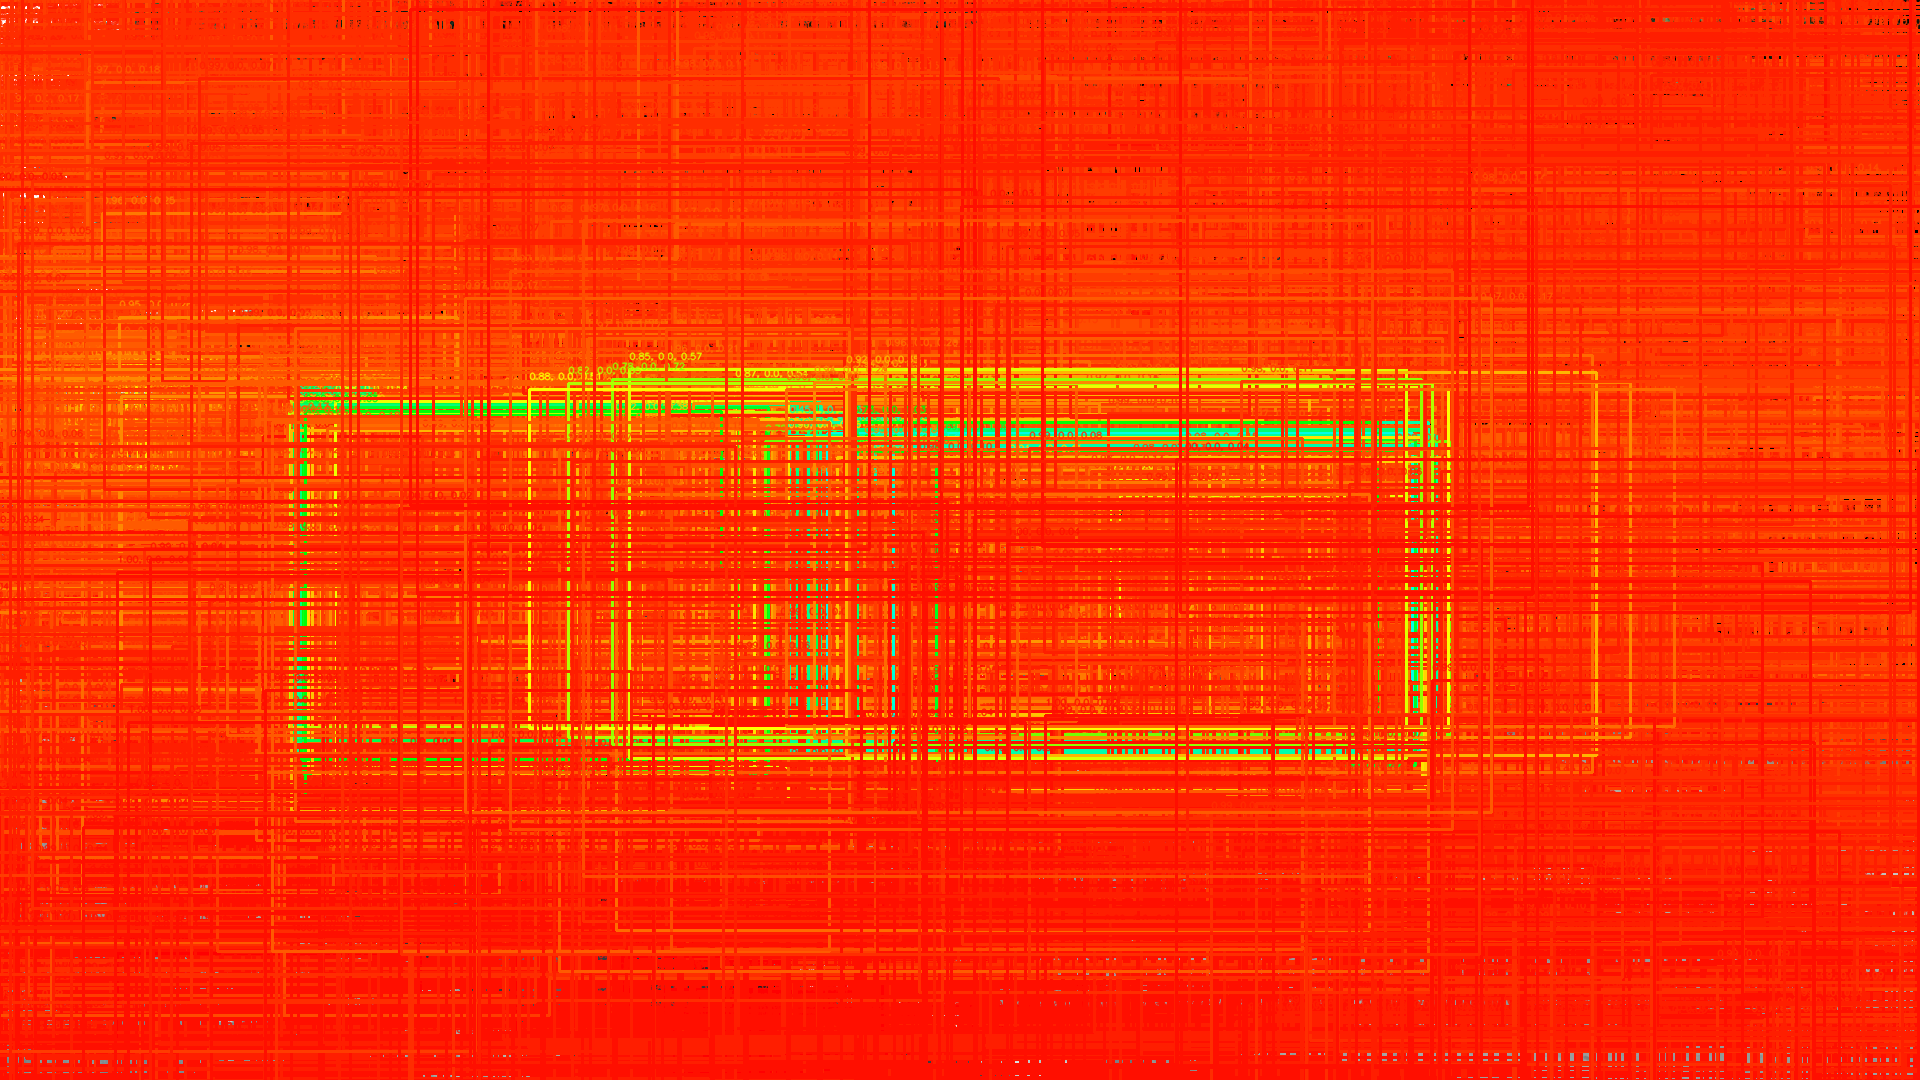
\includegraphics[width=\textwidth]{images/det_images/all_subens_idd_0.png}
               \caption{Visualizing all 8732 boxes regressed by SSD300}
           \end{subfigure}
           \caption{Inference of Bayesian-SSD300 model on a sample image from BDD}
       \end{figure}
\end{frame}

\begin{frame}[allowframebreaks]{UQ models - OOD Detection}
    \begin{figure}[H]
        \captionsetup[table]{skip=0pt}
            \centering
            \begin{subfigure}[t]{0.495\textwidth}
                \centering
                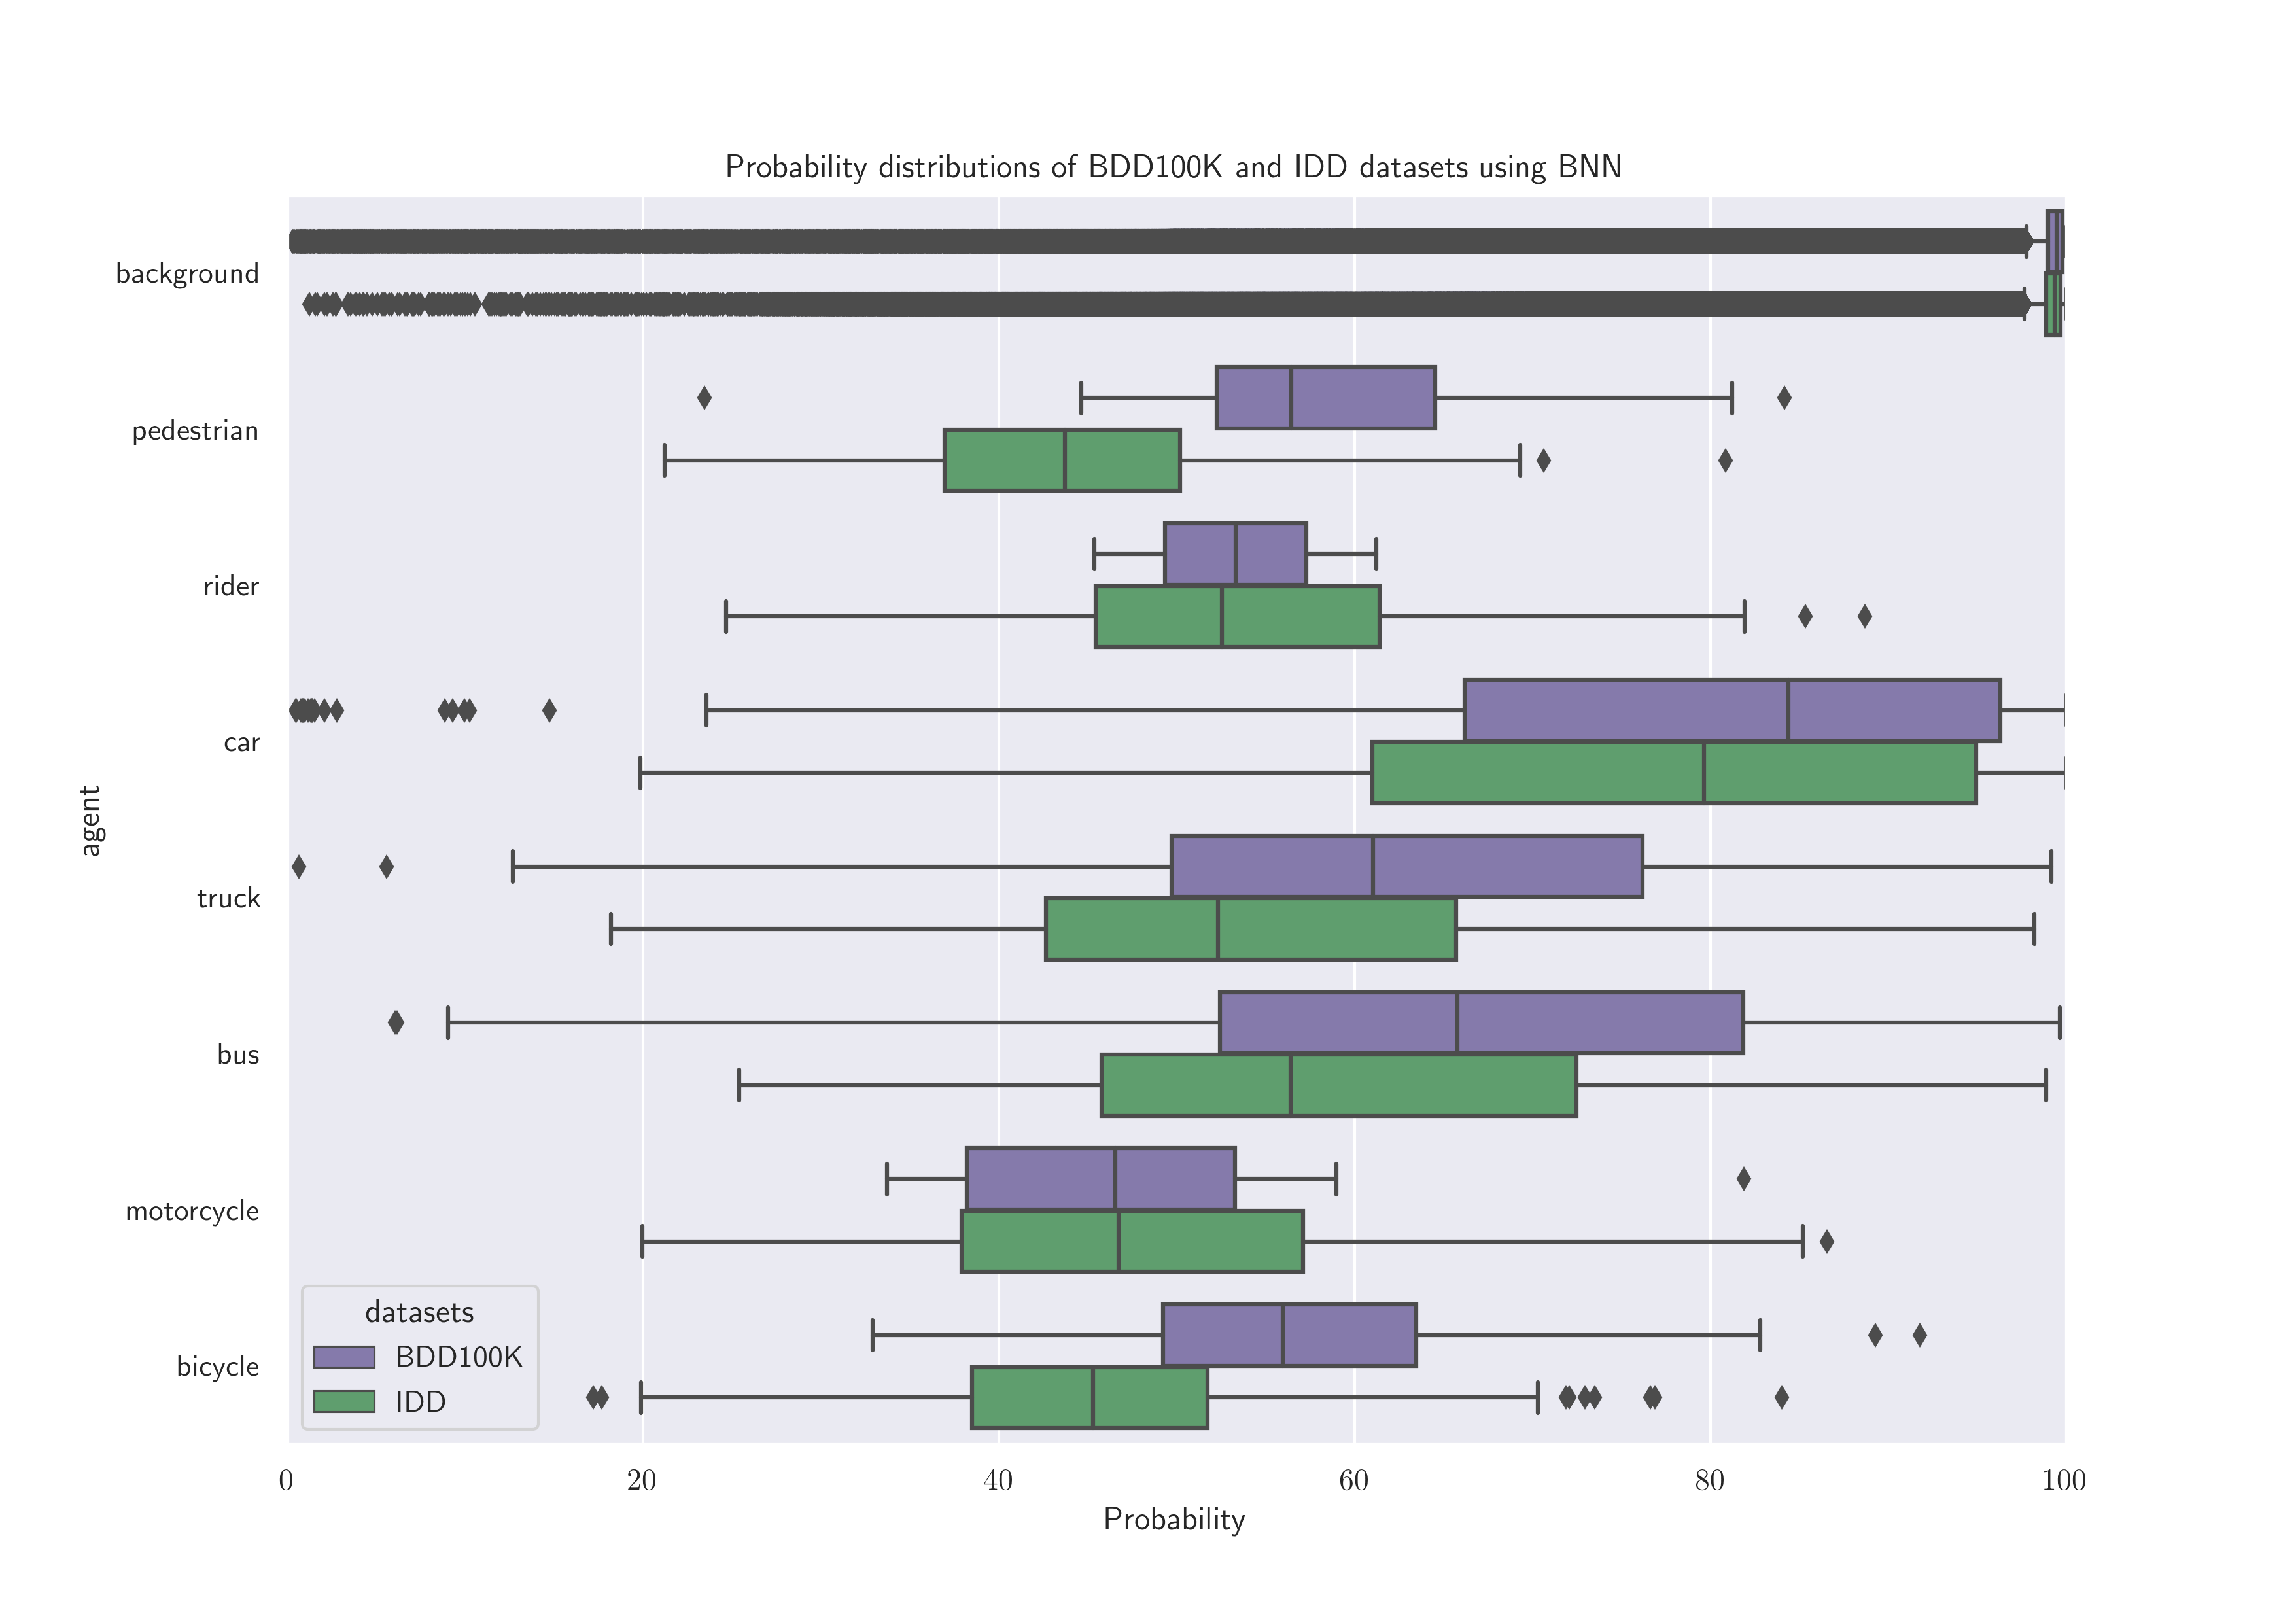
\includegraphics[width=\textwidth]{images/distributions/BNN_bdd_vs_iid_probabilities.png}
                \caption{Detections with variances represented as ellipses}
            \end{subfigure}
            %
            \begin{subfigure}[t]{0.495\textwidth}
                \centering
                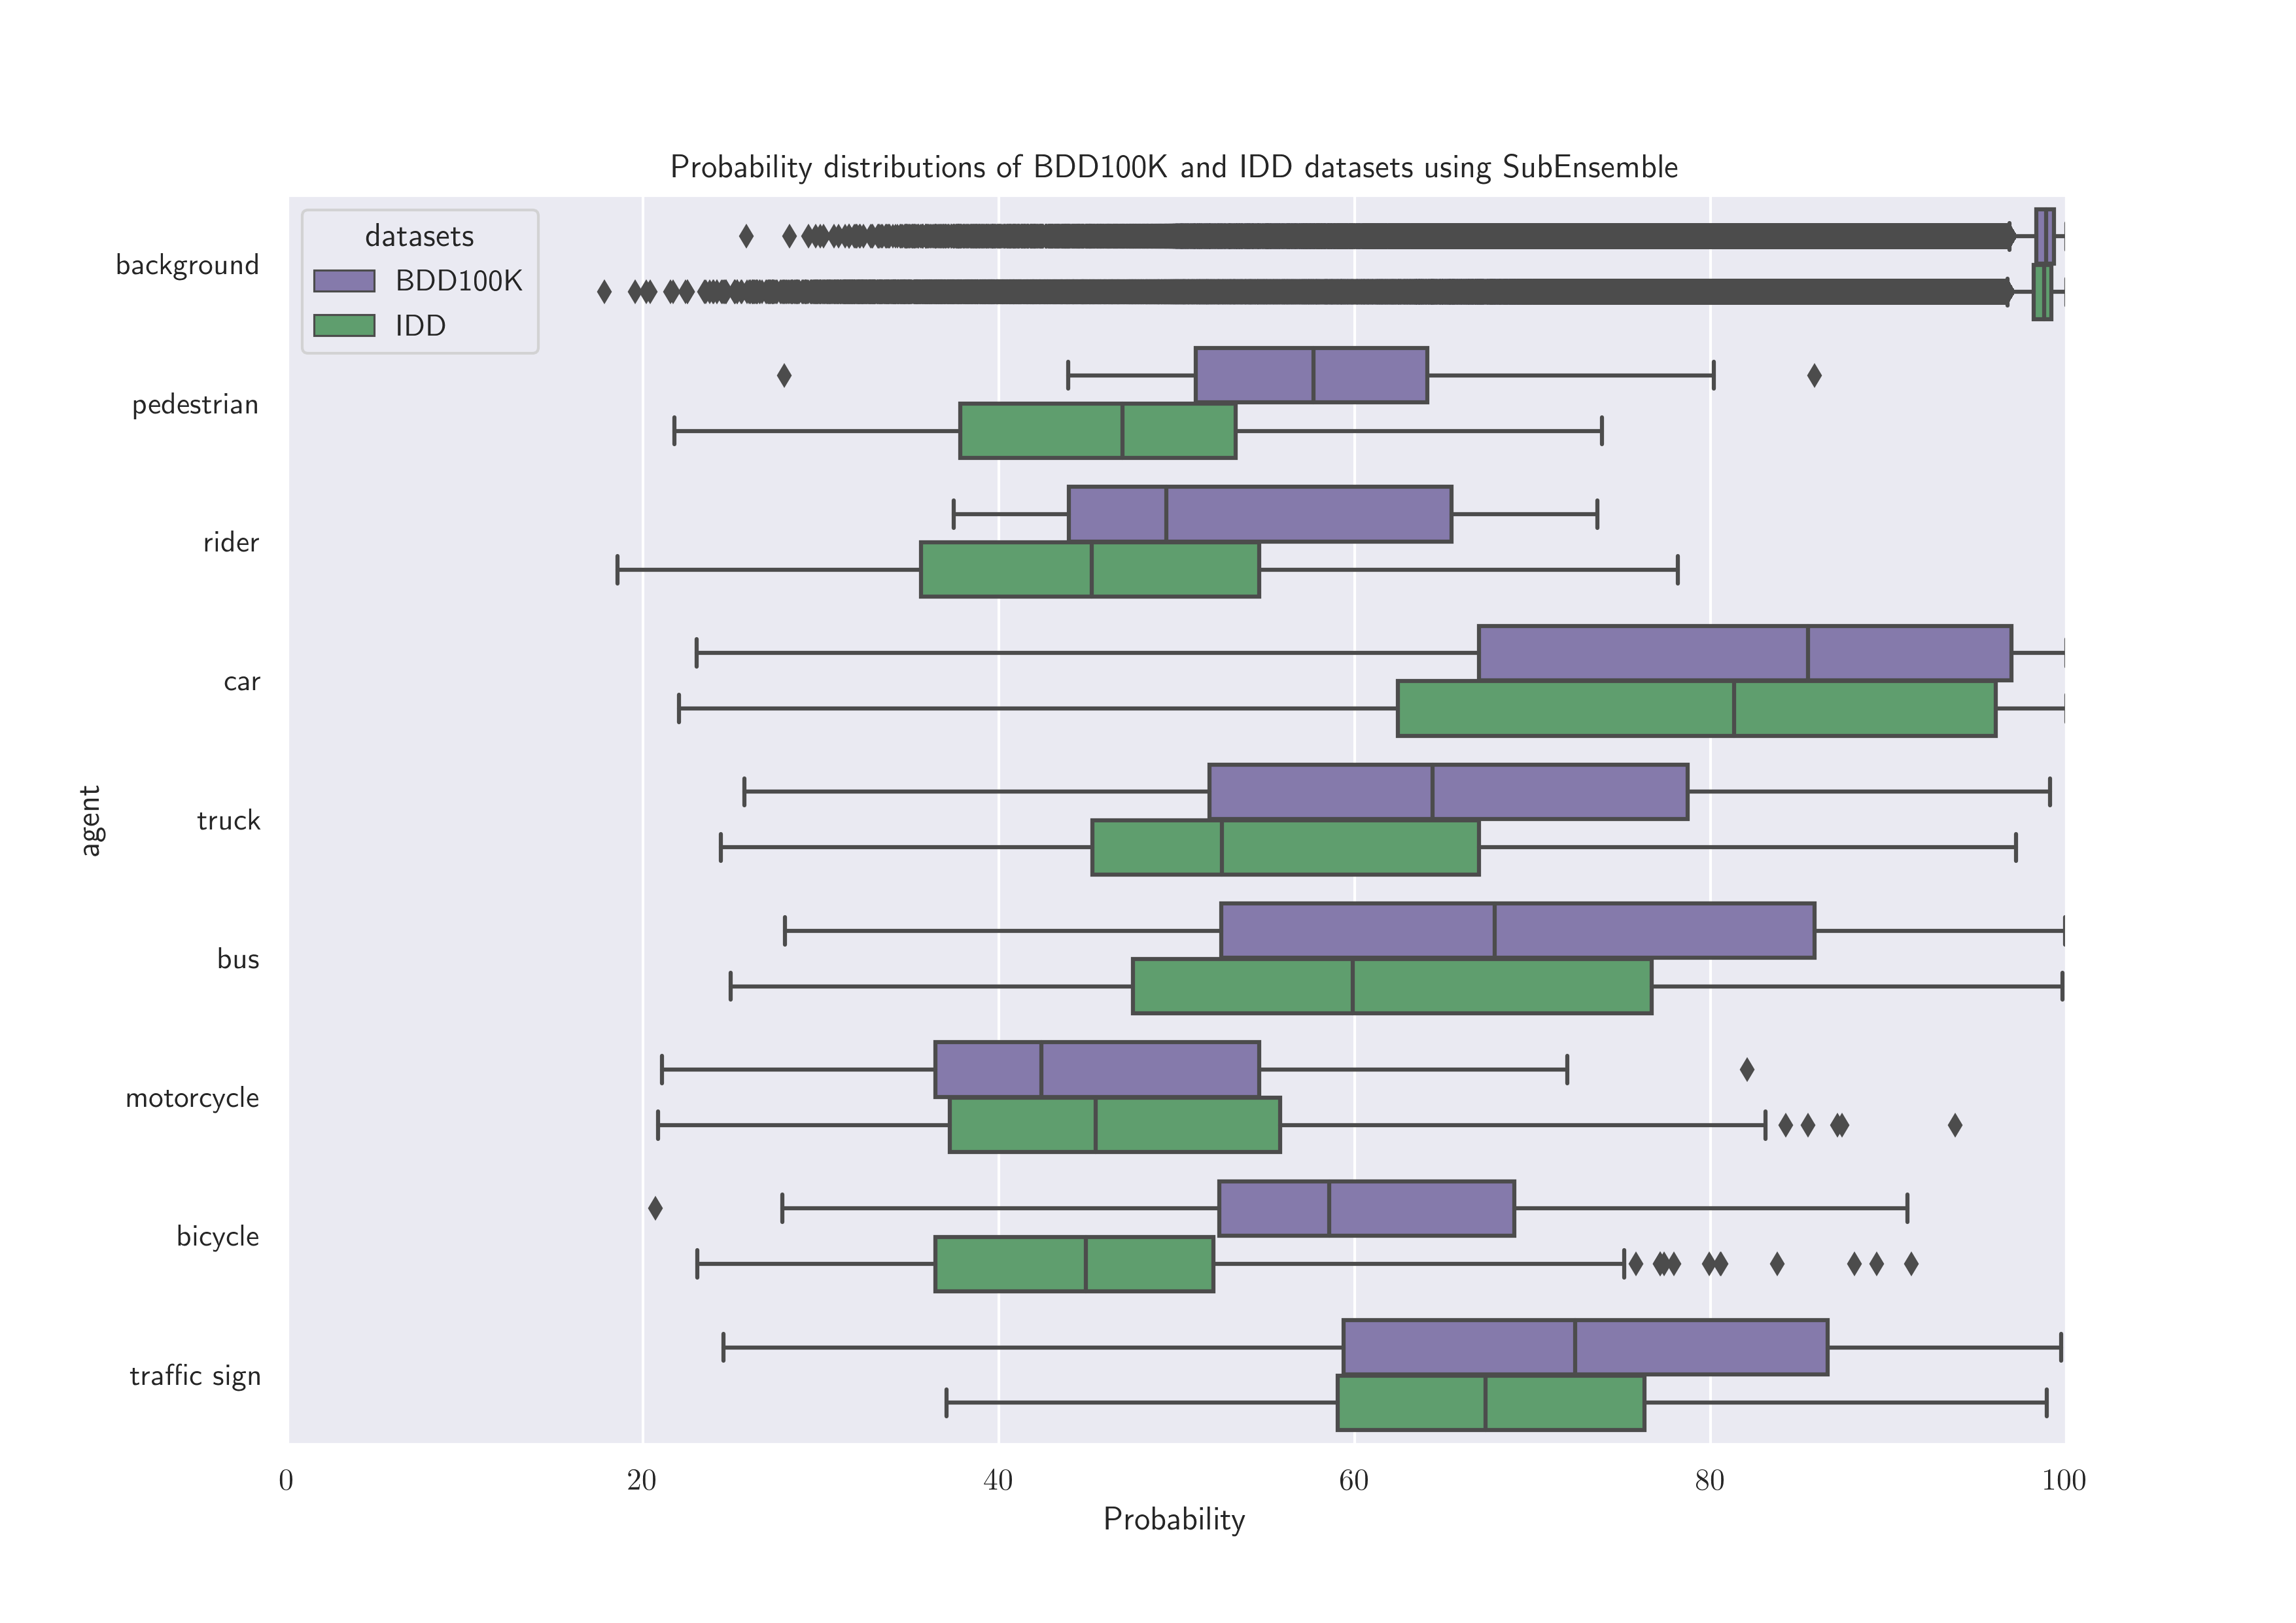
\includegraphics[width=\textwidth]{images/distributions/SubEns_bdd_vs_iid_probabilities.png}
                \caption{Visualizing all 8732 boxes regressed by SSD300}
            \end{subfigure}
            \caption{Inference of Bayesian-SSD300 model on a sample image from BDD}
    \end{figure}

    \begin{figure}[H]
        \captionsetup[table]{skip=0pt}
            \centering
            \begin{subfigure}[t]{0.495\textwidth}
                \centering
                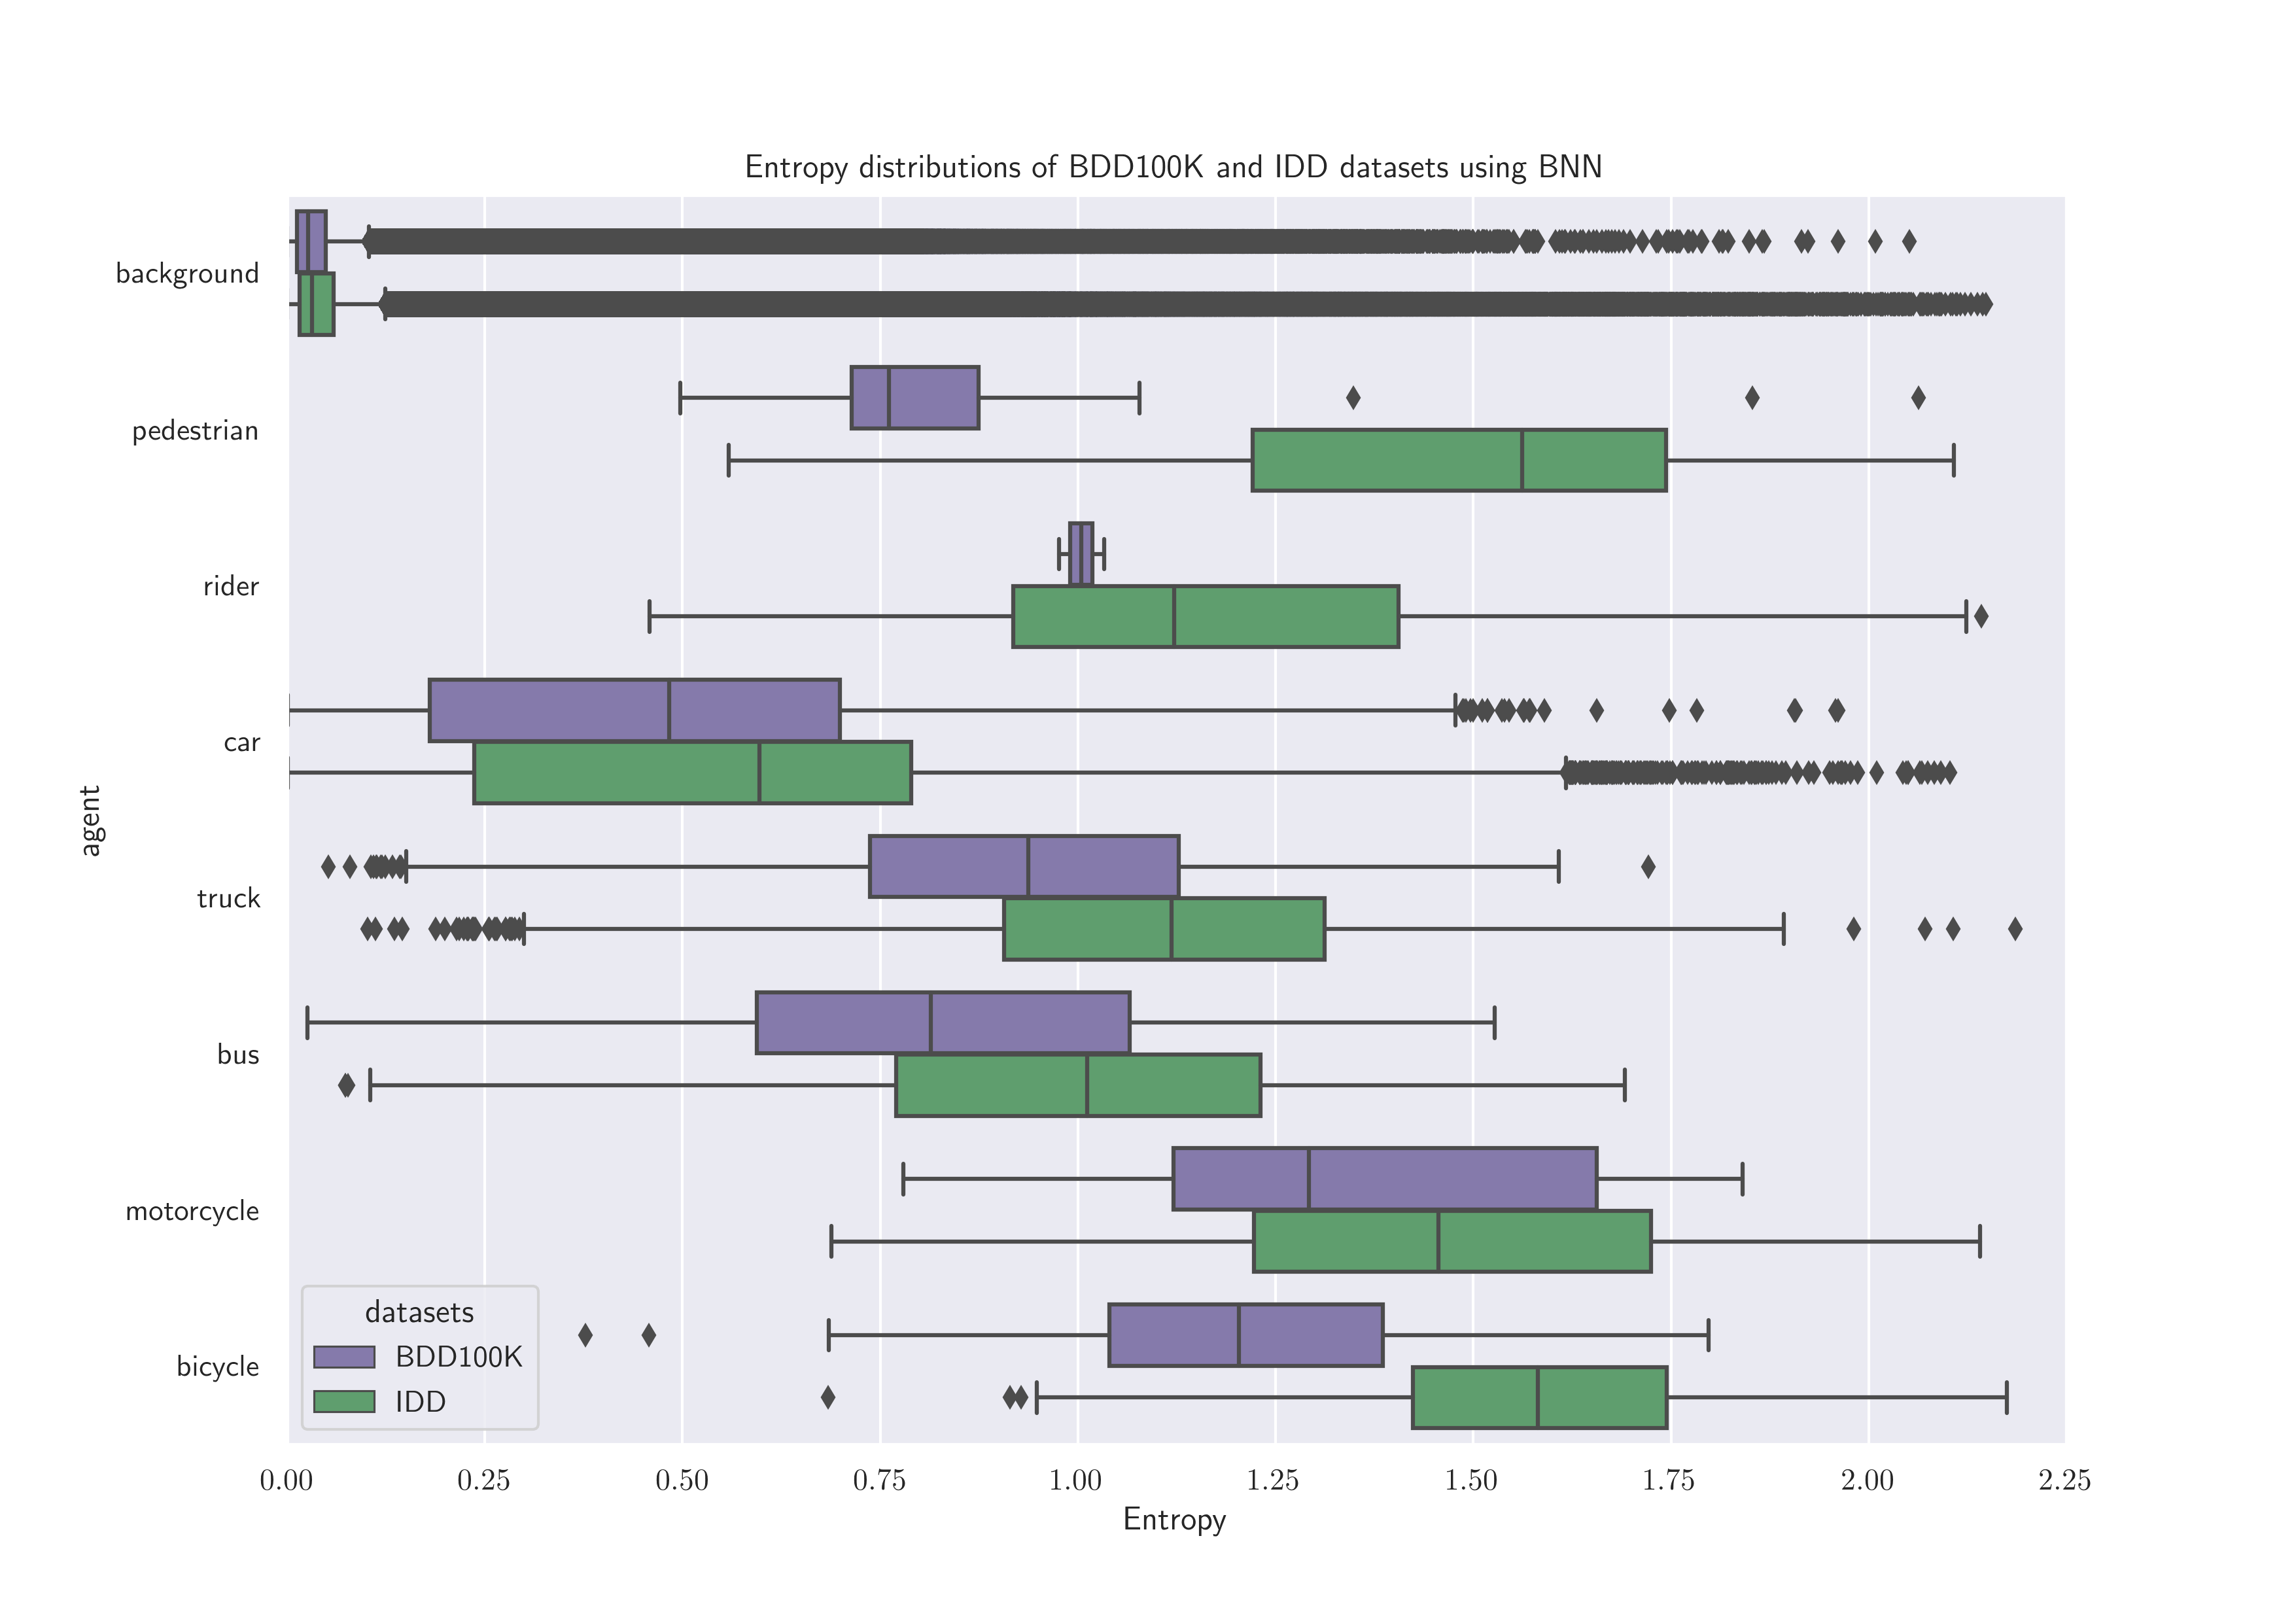
\includegraphics[width=\textwidth]{images/distributions/BNN_bdd_vs_iid_entropy.png}
                \caption{Detections with variances represented as ellipses}
            \end{subfigure}
            %
            \begin{subfigure}[t]{0.495\textwidth}
                \centering
                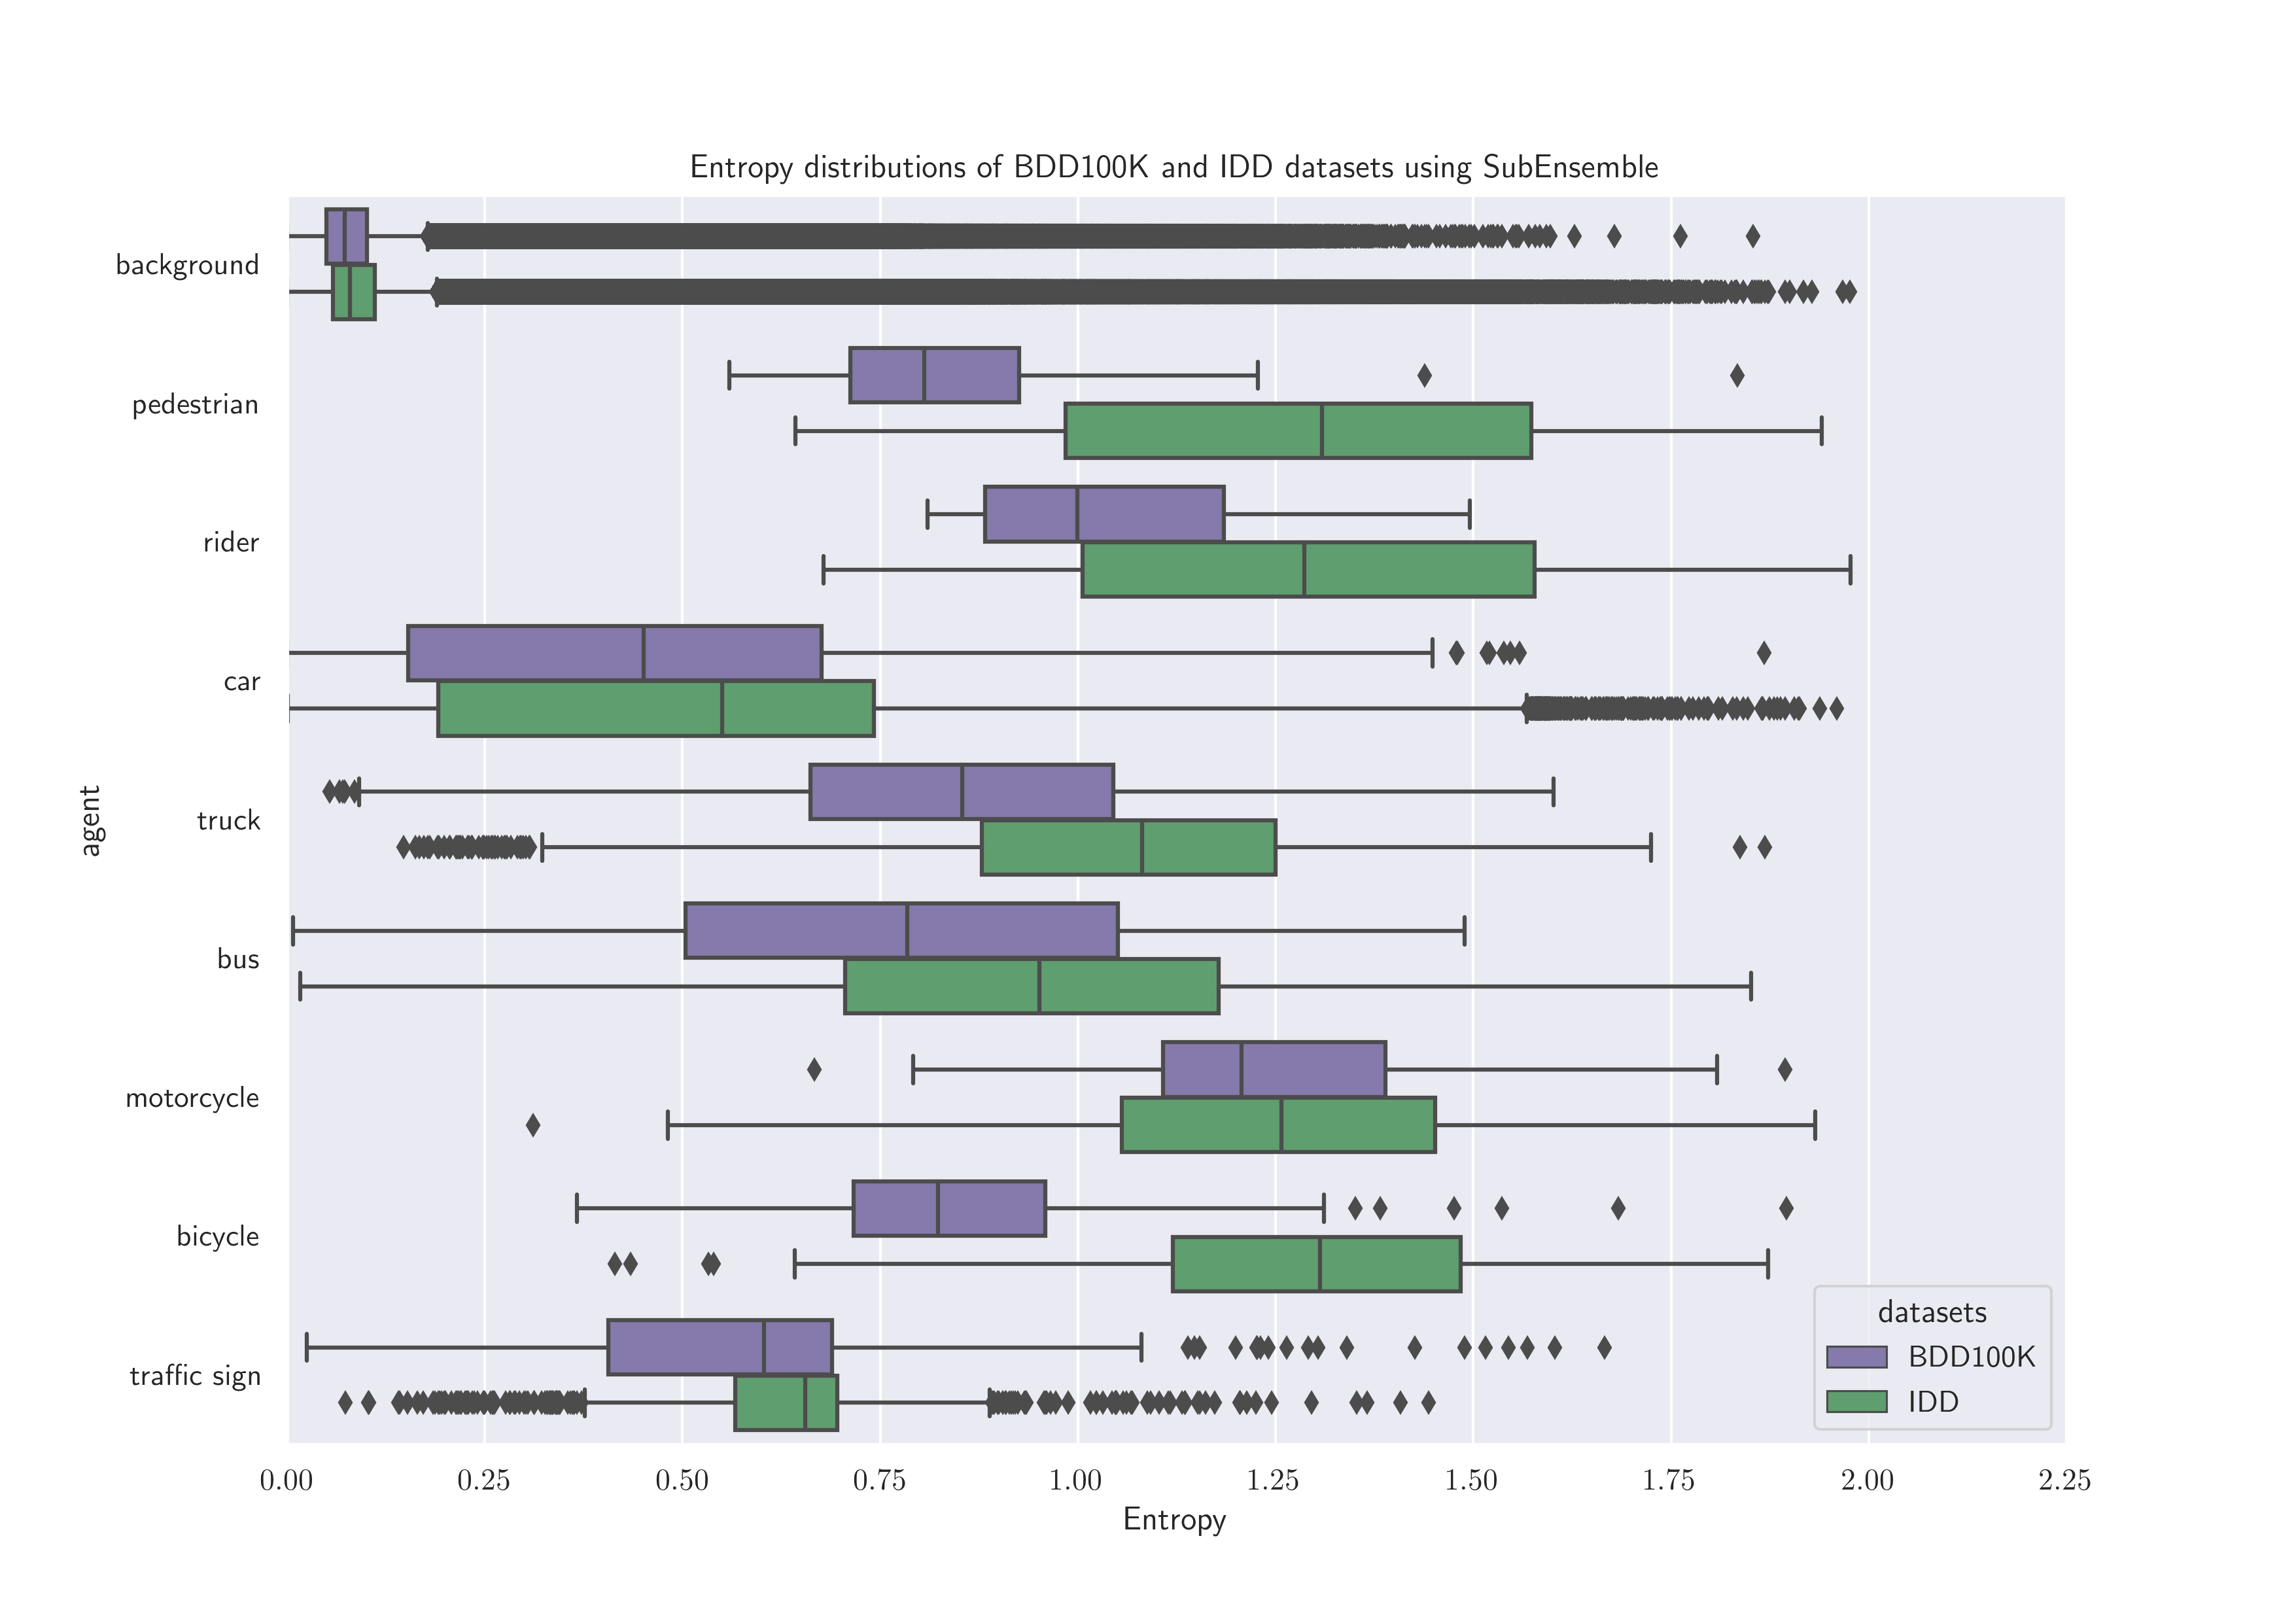
\includegraphics[width=\textwidth]{images/distributions/SubEns_bdd_vs_iid_entropy.png}
                \caption{Visualizing all 8732 boxes regressed by SSD300}
            \end{subfigure}
            \caption{Inference of Bayesian-SSD300 model on a sample image from BDD}
    \end{figure}

    \begin{figure}[H]
        \captionsetup[table]{skip=0pt}
            \centering
            \begin{subfigure}[t]{0.495\textwidth}
                \centering
                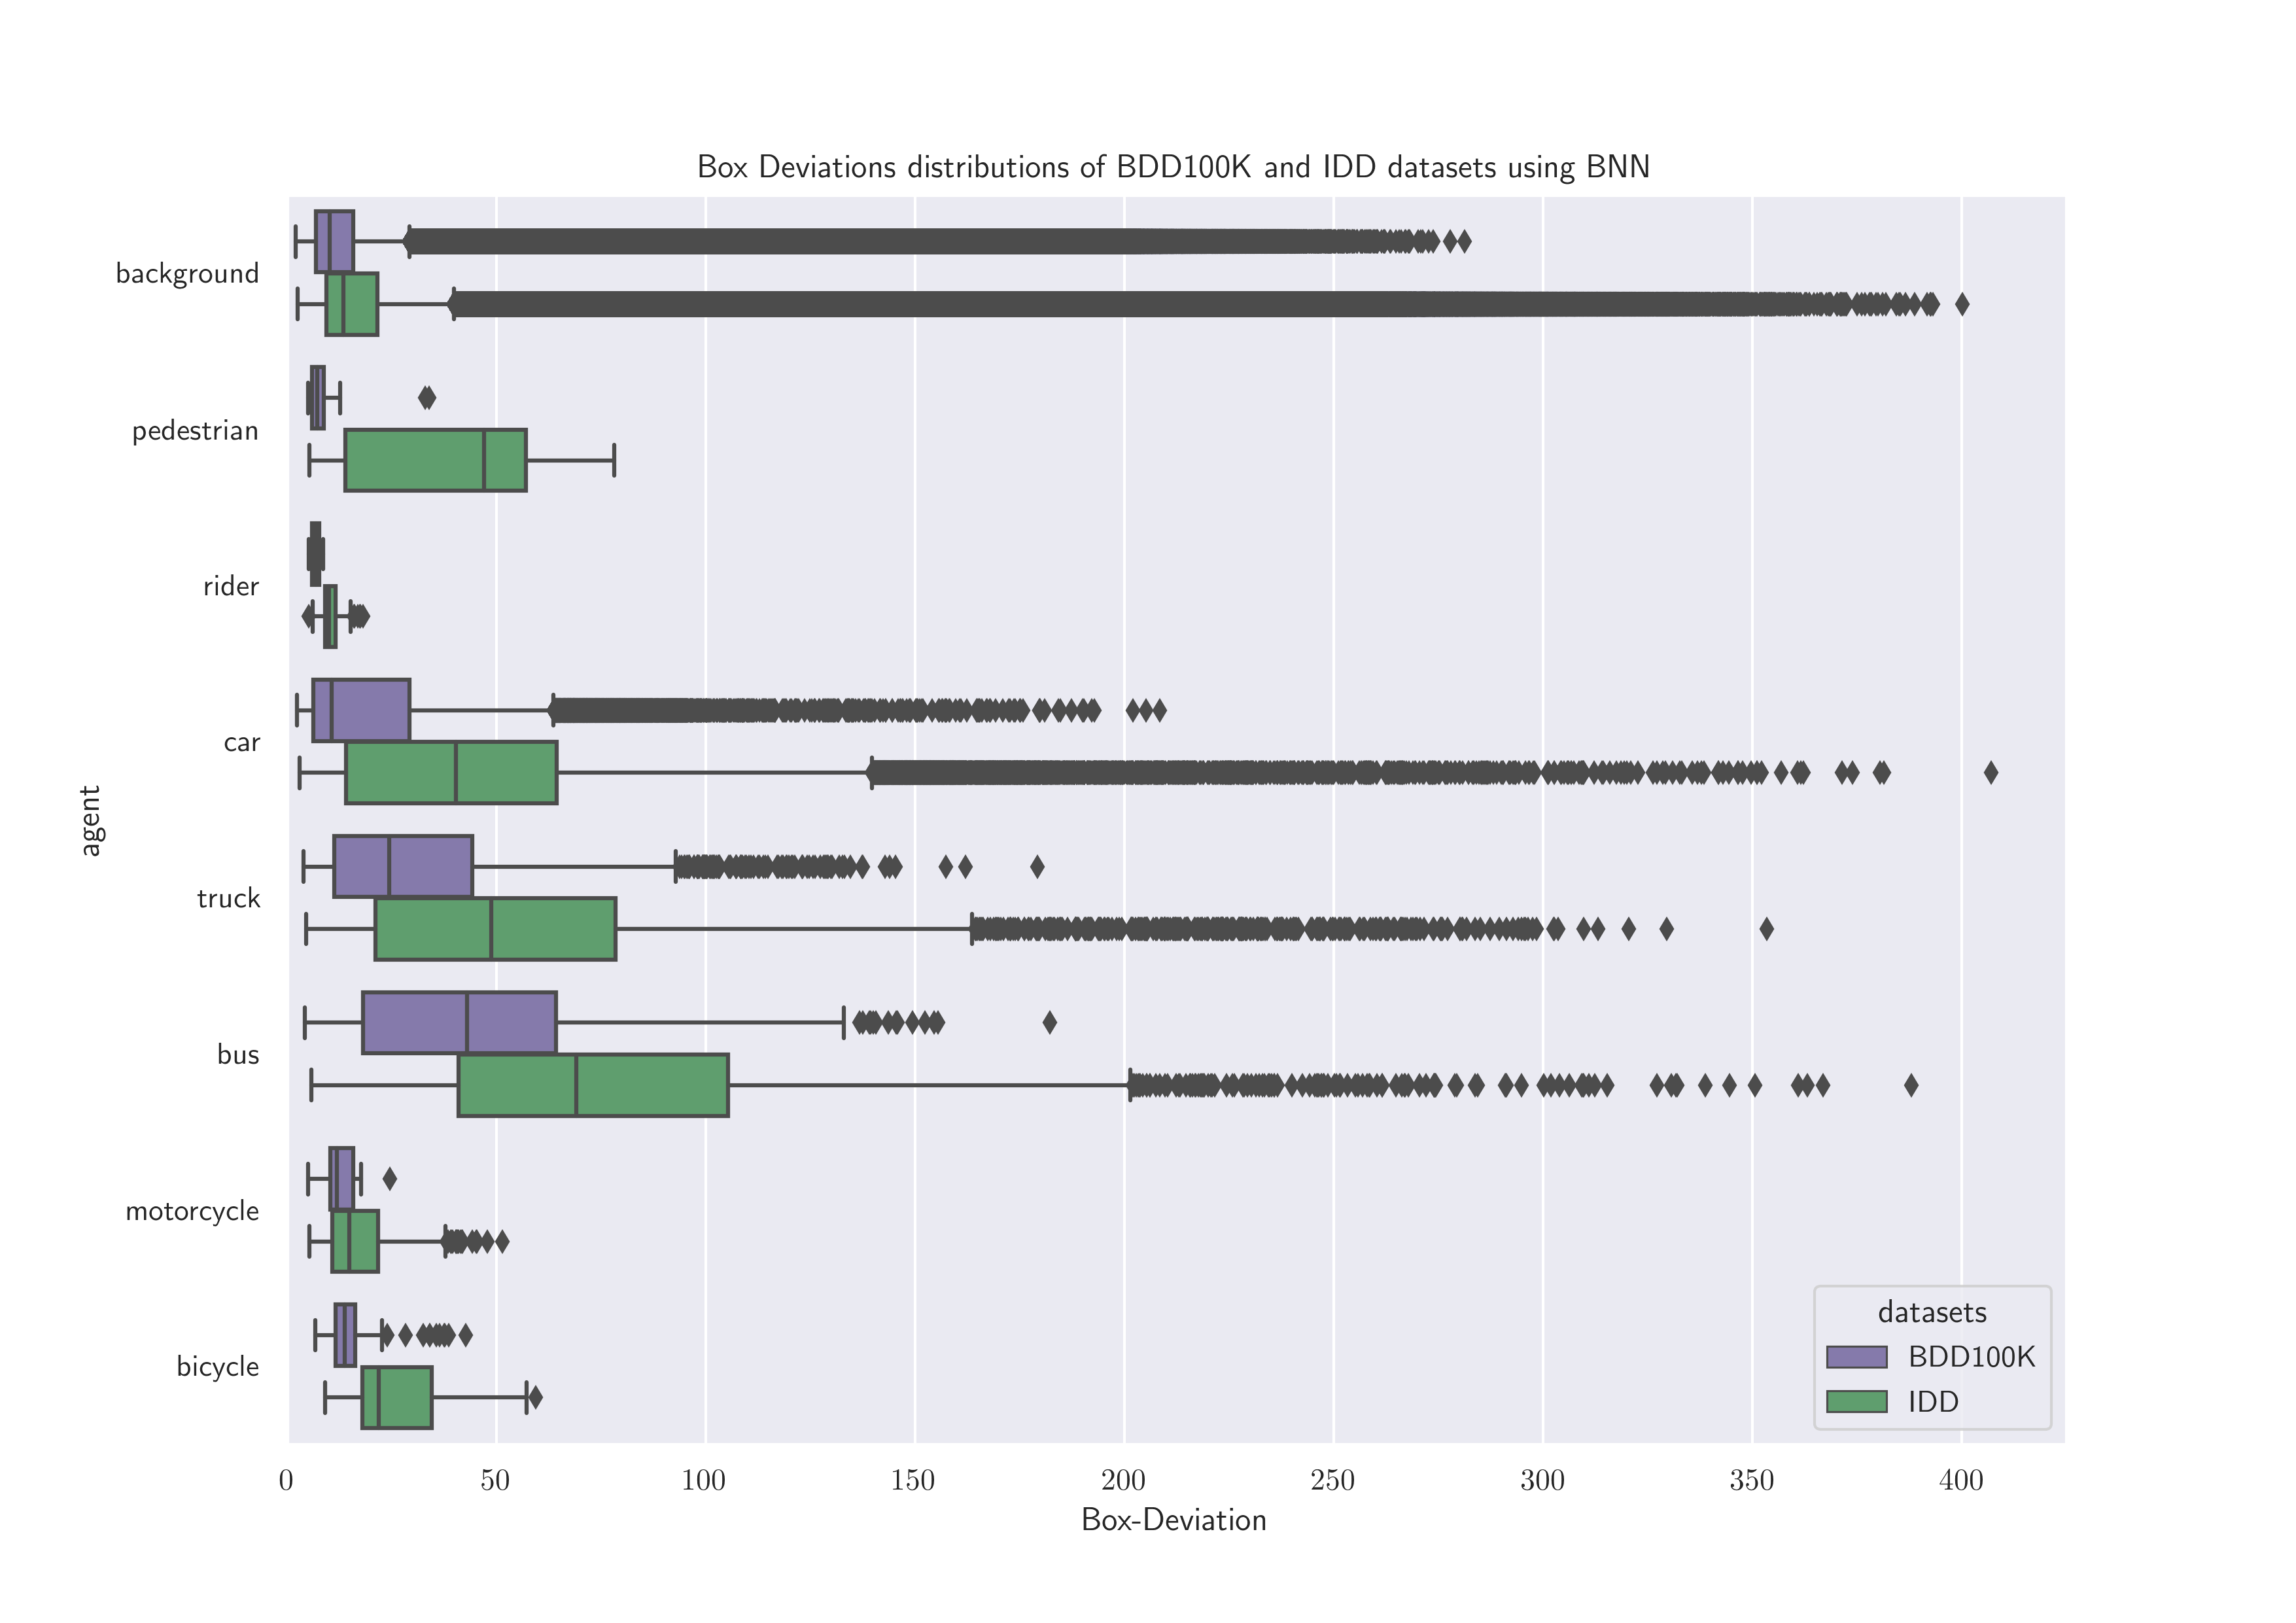
\includegraphics[width=\textwidth]{images/distributions/BNN_bdd_vs_iid_deviations.png}
                \caption{Detections with variances represented as ellipses}
            \end{subfigure}
            %
            \begin{subfigure}[t]{0.495\textwidth}
                \centering
                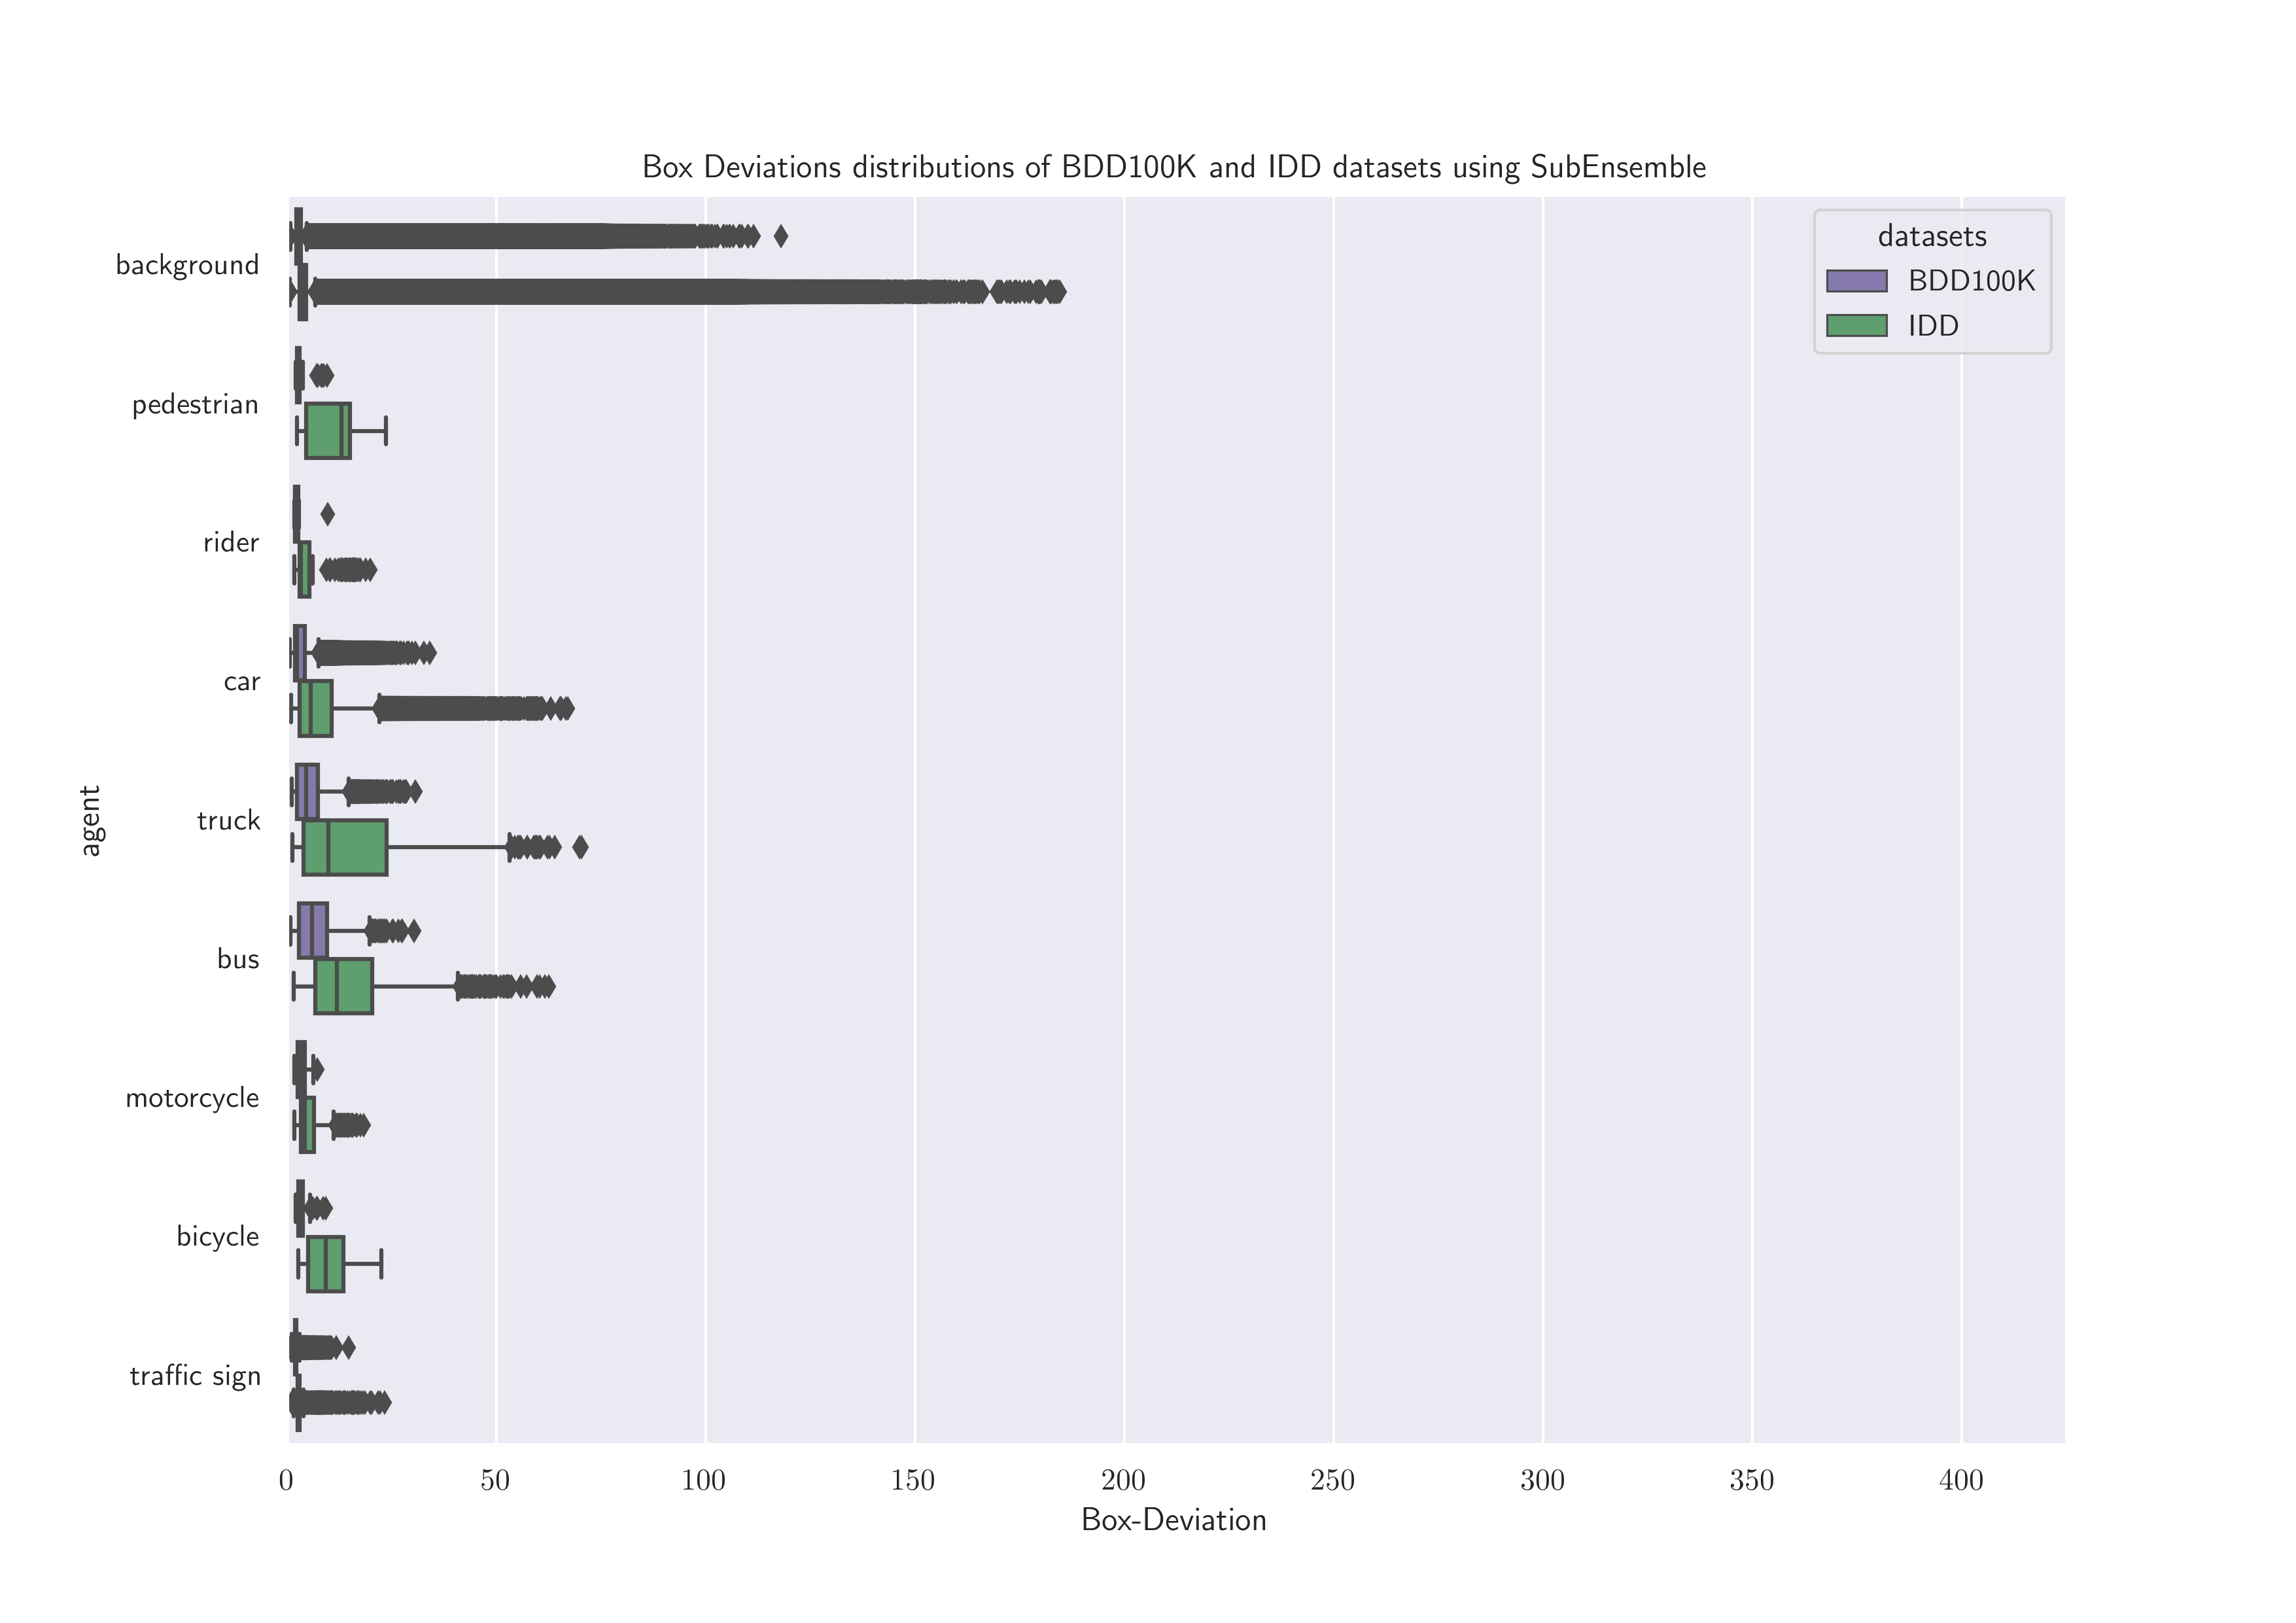
\includegraphics[width=\textwidth]{images/distributions/SubEns_bdd_vs_iid_deviations.png}
                \caption{Visualizing all 8732 boxes regressed by SSD300}
            \end{subfigure}
            \caption{Inference of Bayesian-SSD300 model on a sample image from BDD}
    \end{figure}

    \begin{table}[tbp]
        \centering
        \setlength\abovecaptionskip{-15pt}
        \setlength\belowcaptionskip{0pt}
        \caption{Previous works on OOD detection}
        \resizebox{\textwidth}{!}{%
        \begin{tabular}{lllllllllllc}
        \hline
        \multirow{2}{*}{Models} &
          \multirow{2}{*}{\textbf{Metrics}} &
          \multicolumn{10}{l}{\textbf{Agents}} \\ \cline{3-12} 
         &
           &
          Background &
          Pedestrian &
          Rider &
          Car &
          Truck &
          Bus &
          Motorcycle &
          Bicycle &
          Traffic Sign &
          Mean \\ \hline
        \multirow{3}{*}{Bayesian-SSD300} &
          Probability &
          0.45 &
          0.14 &
          0.75 &
          0.45 &
          0.37 &
          0.38 &
          0.49 &
          0.23 &
          - &
          \multicolumn{1}{l}{0.45} \\ \cline{2-12} 
         &
          Entropy &
          0.56 &
          0.88 &
          0.59 &
          0.59 &
          0.67 &
          0.64 &
          0.6 &
          0.84 &
          - &
          0.56 \\ \cline{2-12} 
         &
          Box\_deviation &
          0.64 &
          0.93 &
          0.82 &
          0.76 &
          0.69 &
          0.7 &
          0.62 &
          0.85 &
          - &
          0.64 \\ \hline
        \multirow{3}{*}{\begin{tabular}[c]{@{}l@{}}Sub-Ensemble\\ SSD300\end{tabular}} &
          Probability &
          0.44 &
          0.21 &
          0.34 &
          0.46 &
          0.34 &
          0.4 &
          0.53 &
          0.19 &
          0.41 &
          0.44 \\ \cline{2-12} 
         &
          Entropy &
          0.56 &
          0.86 &
          0.72 &
          0.58 &
          0.71 &
          0.62 &
          0.51 &
          0.88 &
          0.62 &
          \multicolumn{1}{l}{0.56} \\ \cline{2-12} 
         &
          Box\_deviation &
          0.76 &
          0.95 &
          0.84 &
          0.79 &
          0.74 &
          0.75 &
          0.71 &
          0.94 &
          0.88 &
          \multicolumn{1}{l}{0.75} \\ \hline
        \end{tabular}%
        }
        \end{table}
        \begin{columns}
            \column{0.45\linewidth}
                \begin{itemize}
                    \item metrics struggled in classifying background class between ID and OOD data.
                    \item Box deviation performed well in detecting OOD.
                \end{itemize}
            \column{0.45\linewidth}
                \begin{itemize}
                    \item performance is similar in Car, Truck, Bus, and Rider 
                \end{itemize}
        \end{columns}
        \pagebreak

        \begin{columns}
            \begin{column}{.2\textwidth}
                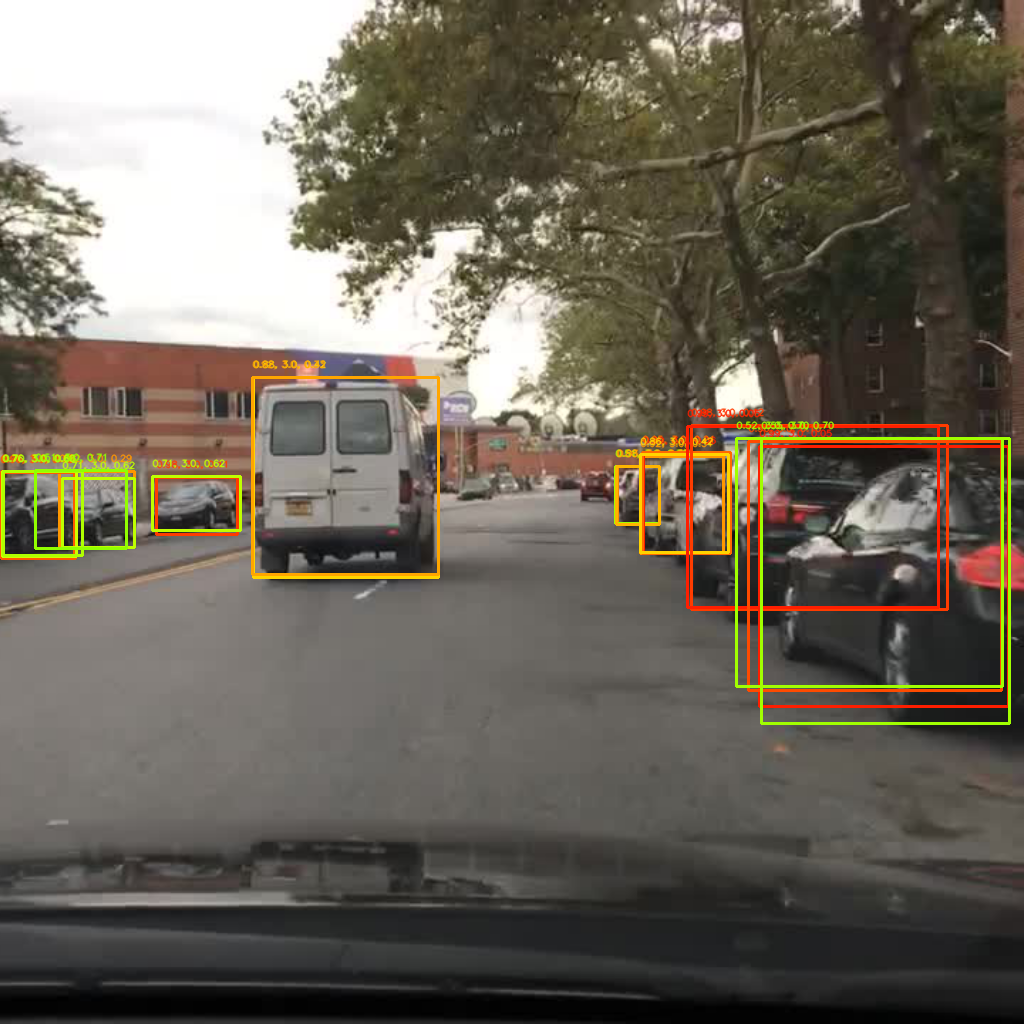
\includegraphics[width=\textwidth]{images/uq_weathers/BNN_variances2.png}
                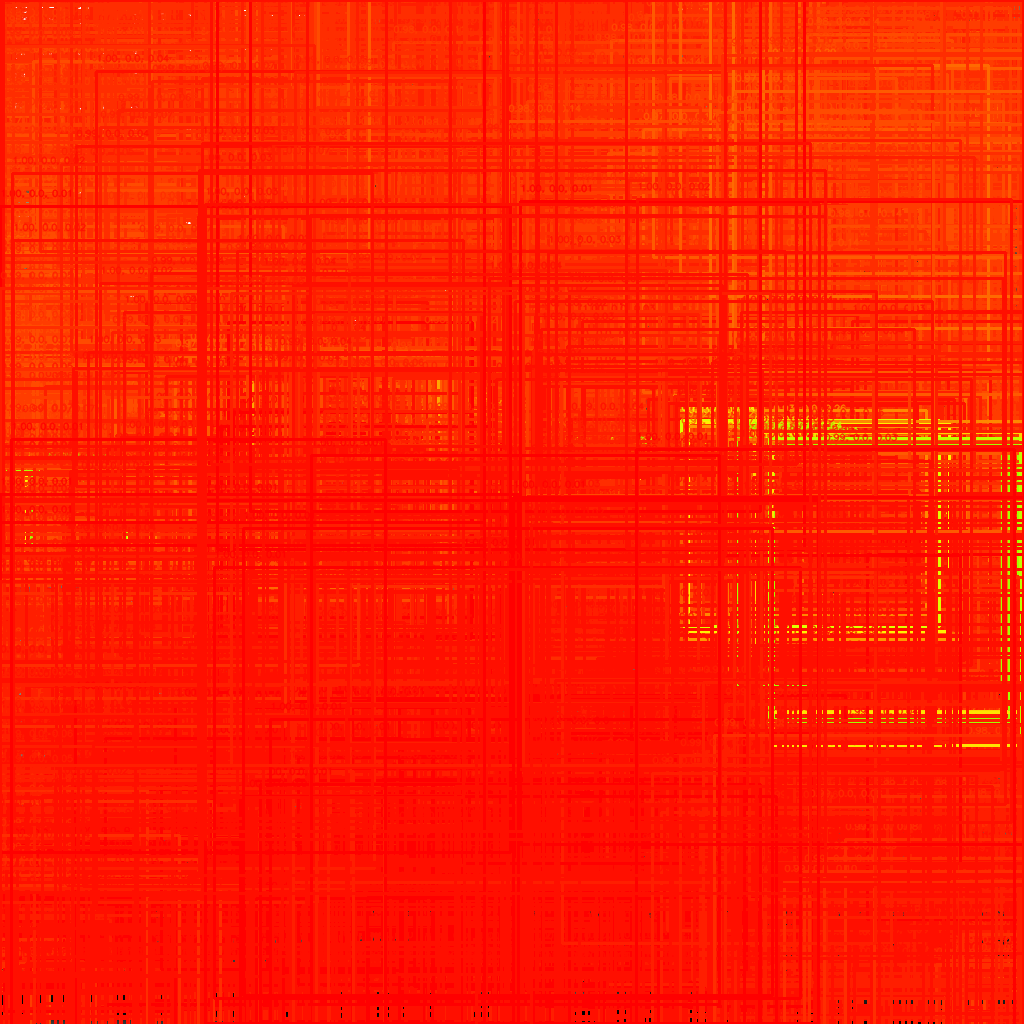
\includegraphics[width=\textwidth]{images/uq_weathers/flipout_entropies_all2.png}
            \end{column}
            \begin{column}{.2\textwidth}
                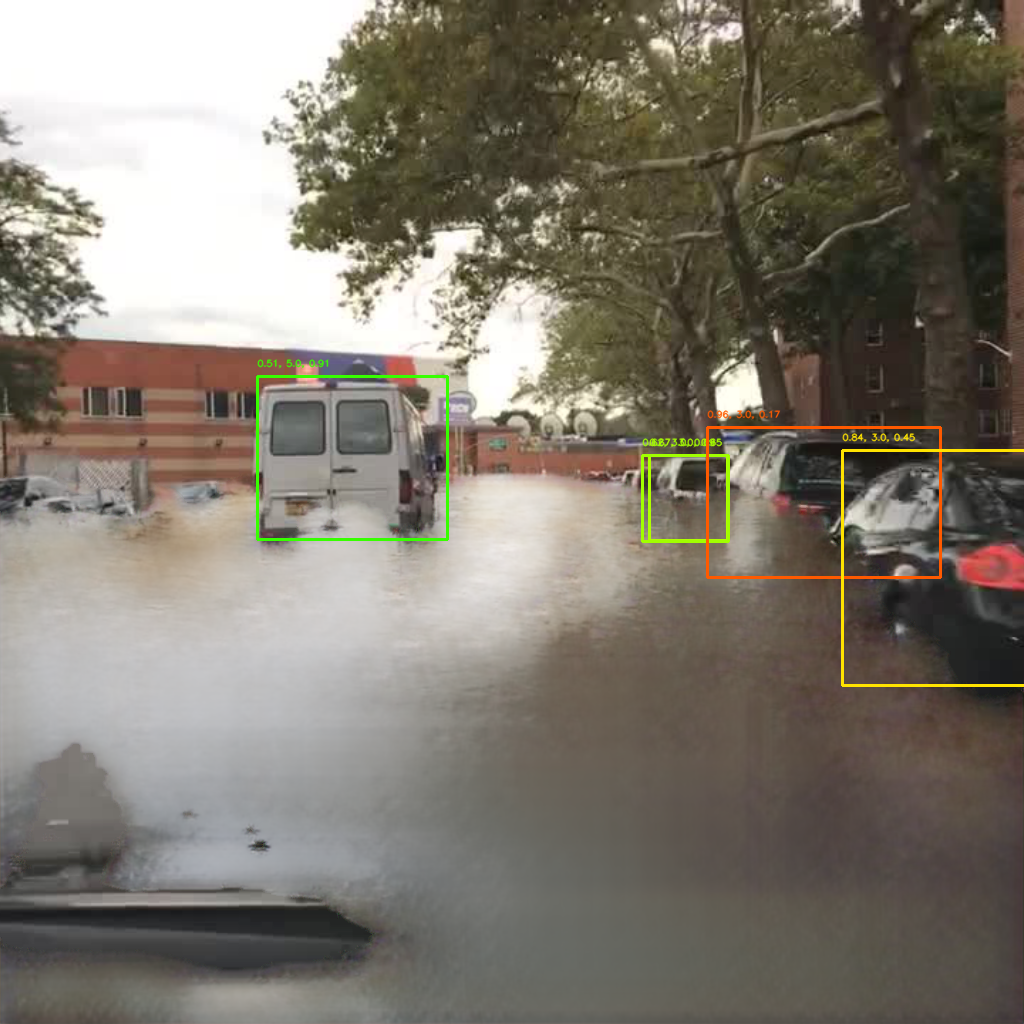
\includegraphics[width=\textwidth]{images/uq_weathers/BNN_variances1.png}
                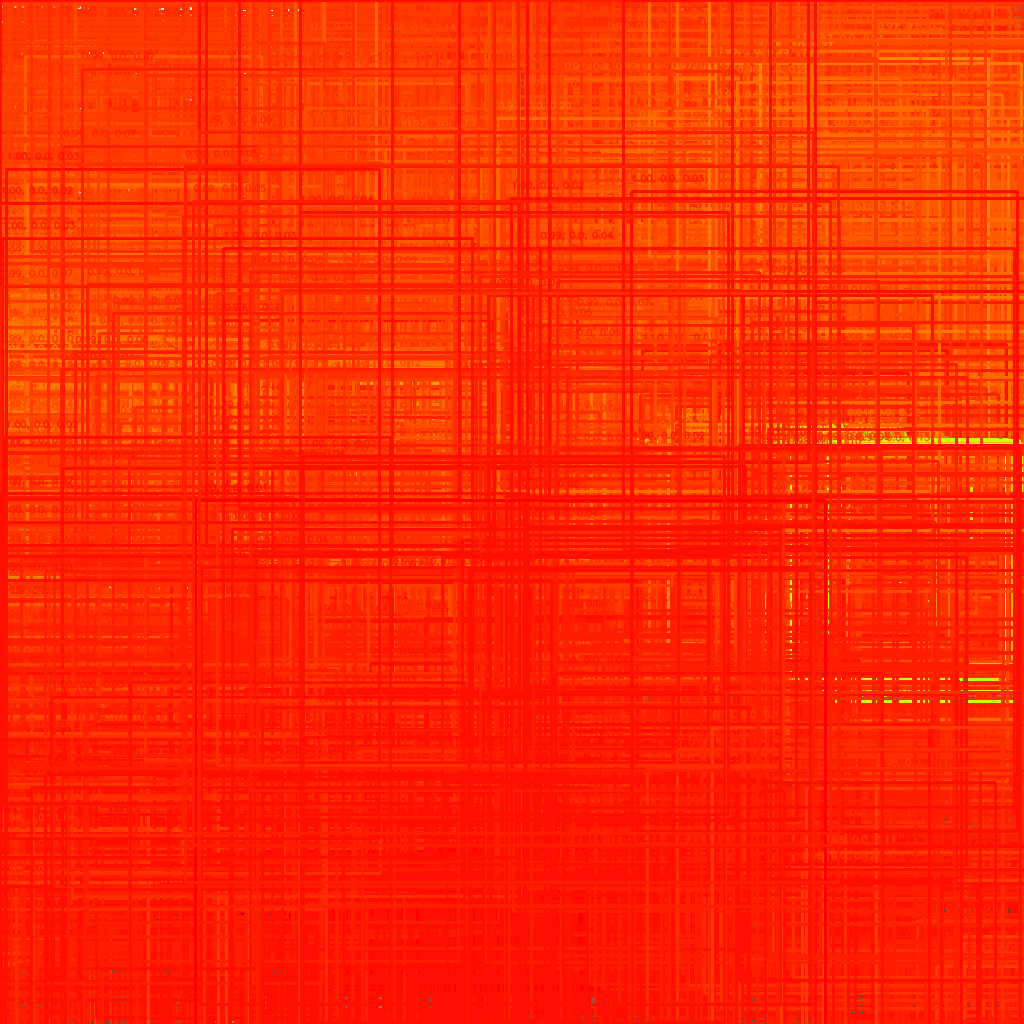
\includegraphics[width=\textwidth]{images/uq_weathers/flipout_entropies_all1.png}
            \end{column}
            \begin{column}{.2\textwidth}
                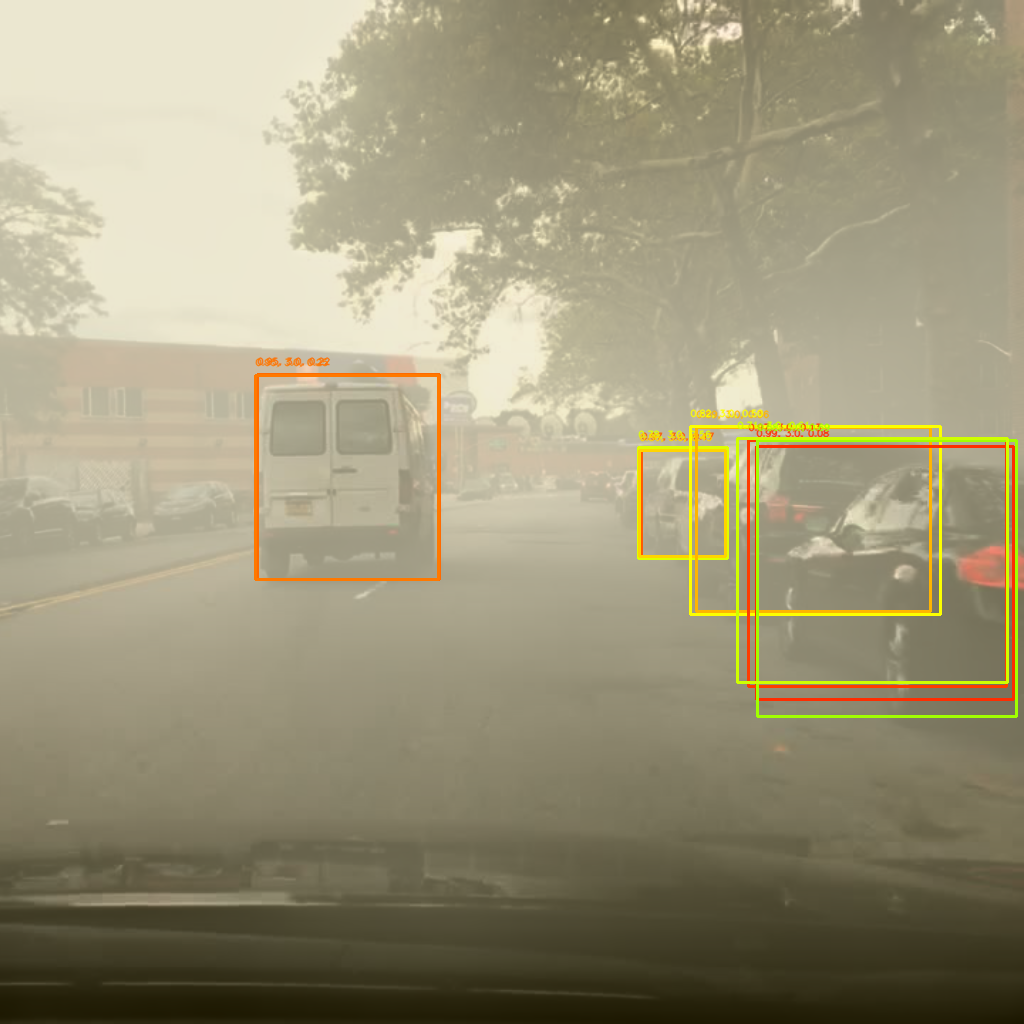
\includegraphics[width=\textwidth]{images/uq_weathers/BNN_variances3.png}
                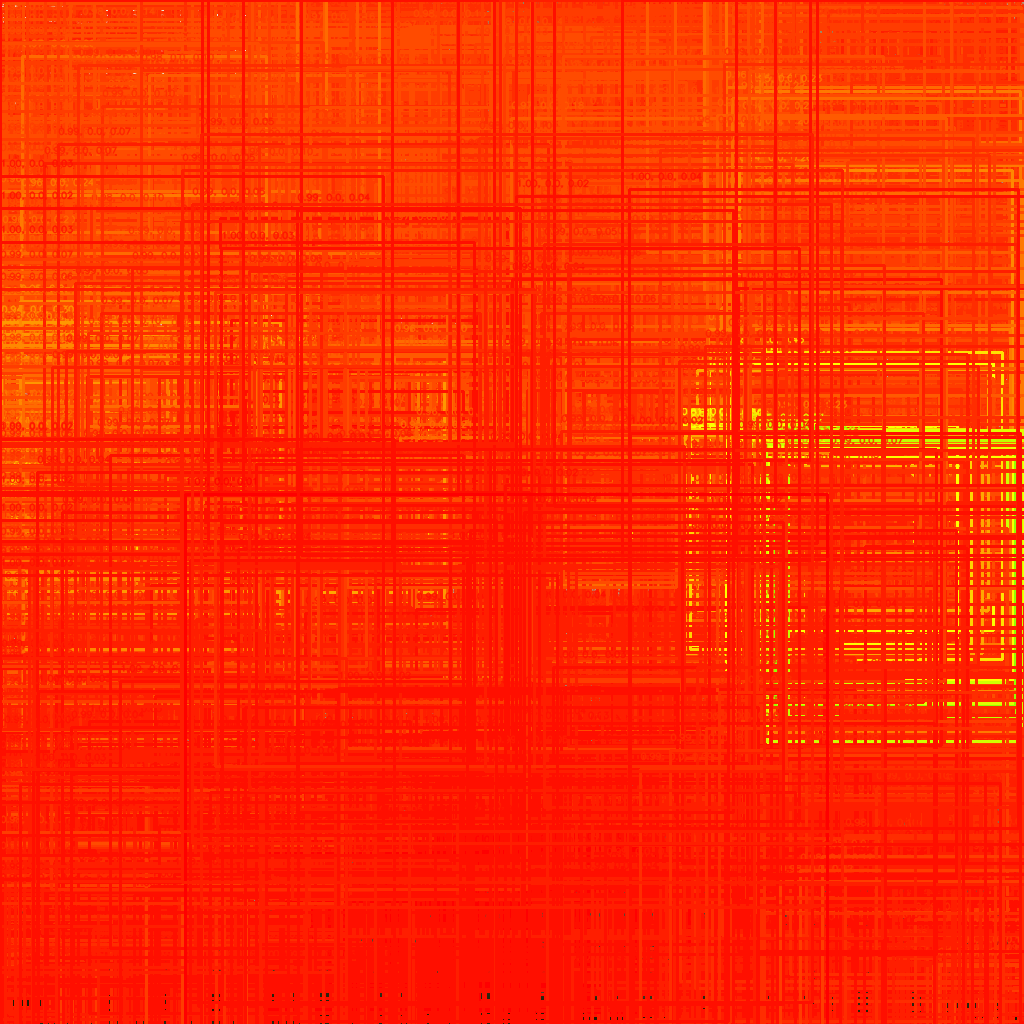
\includegraphics[width=\textwidth]{images/uq_weathers/flipout_entropies_all3.png}
            \end{column}
            \begin{column}{.2\textwidth}
                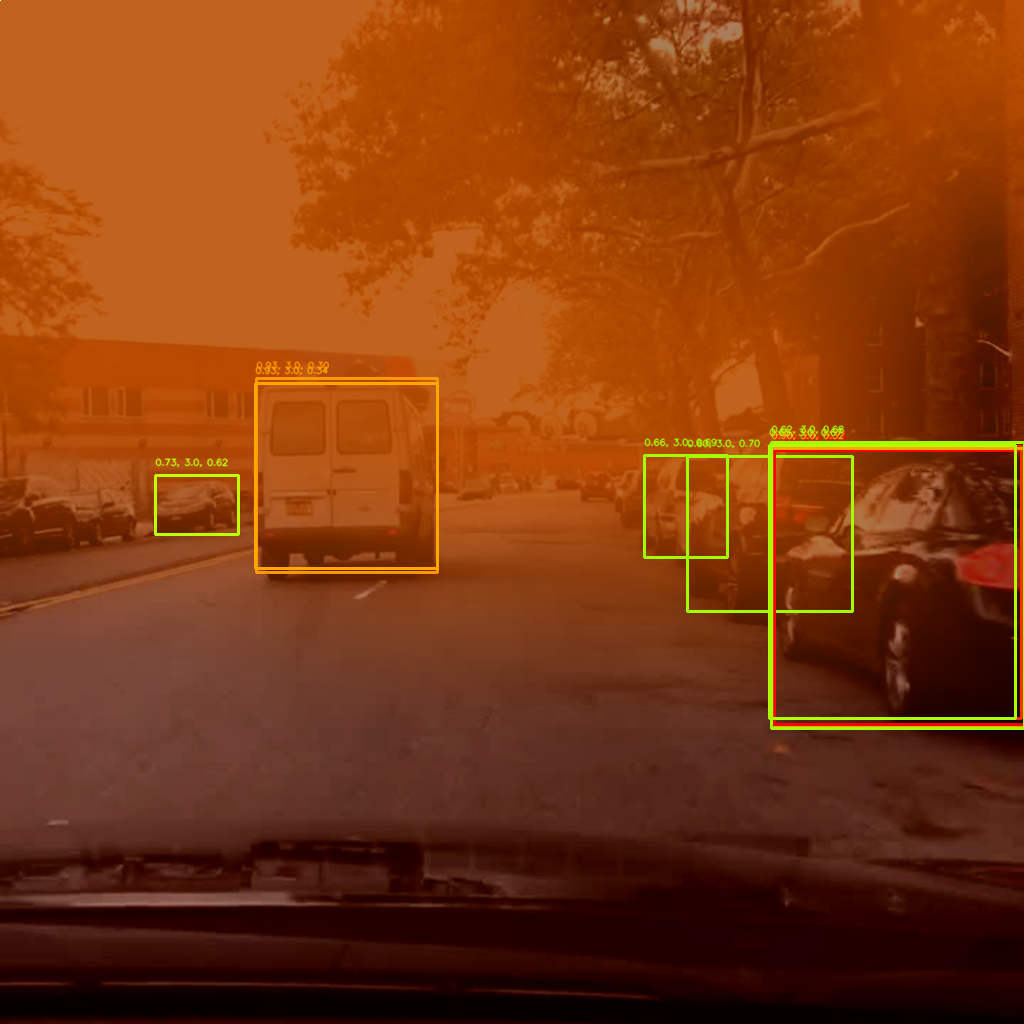
\includegraphics[width=\textwidth]{images/uq_weathers/BNN_variances4.png}
                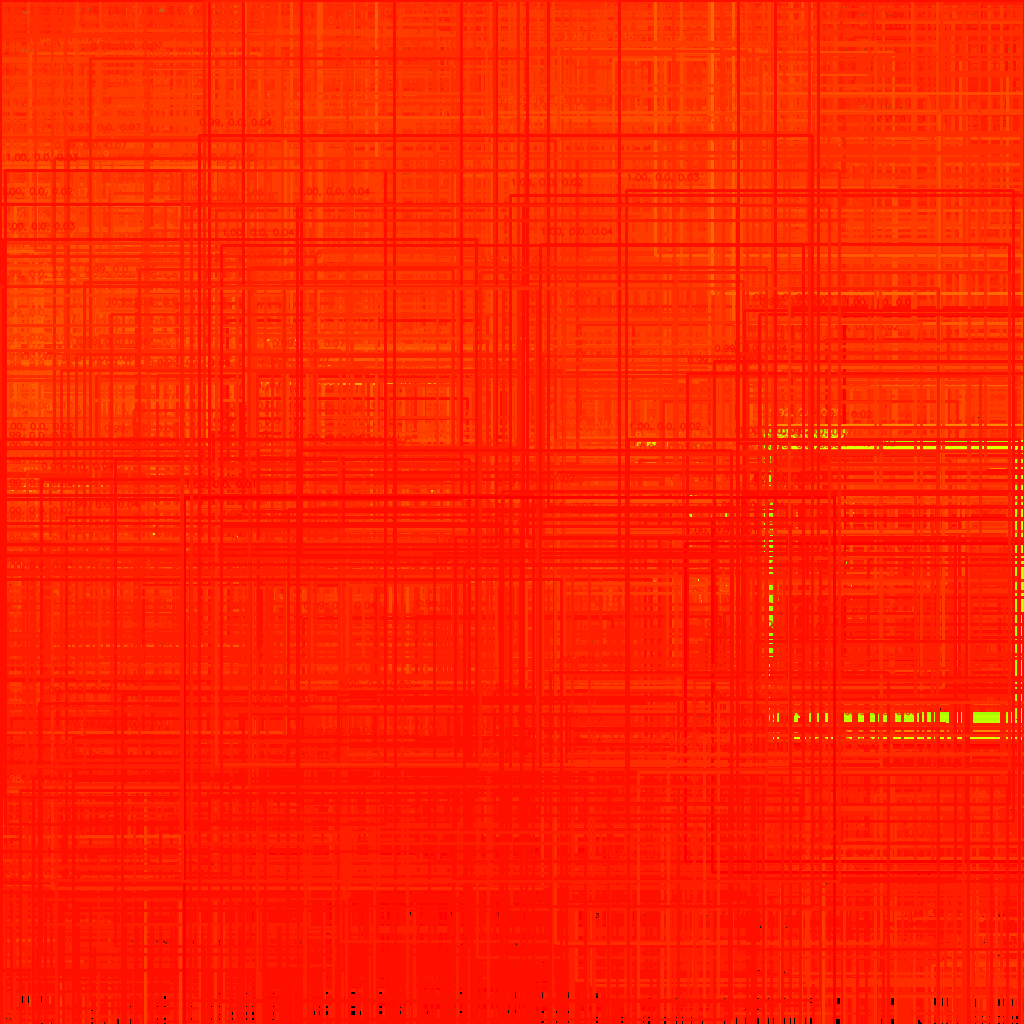
\includegraphics[width=\textwidth]{images/uq_weathers/flipout_entropies_all4.png}
            \end{column}
        \end{columns}
        \begin{center}
            Performance of BNN on BDD100K weather dataset
        \end{center}
        

        \begin{columns}
            \begin{column}{.2\textwidth}
                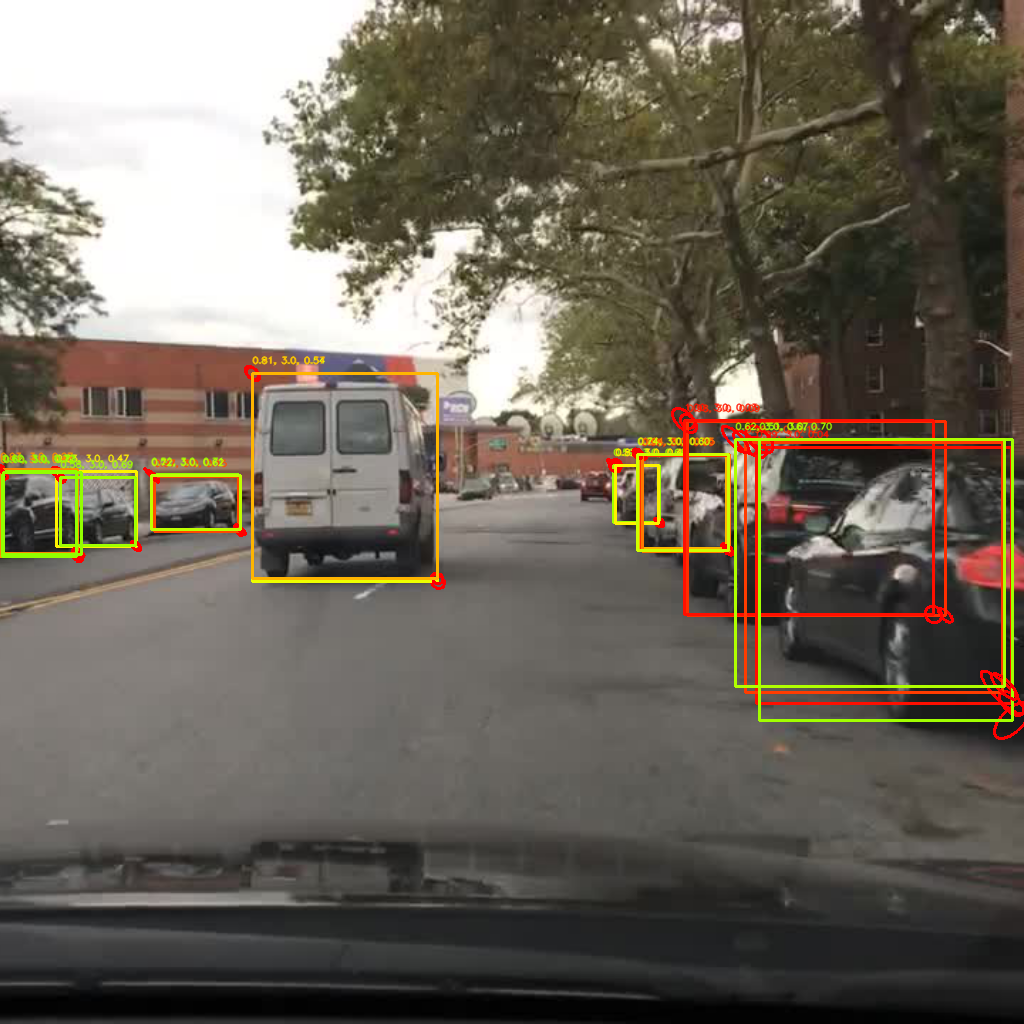
\includegraphics[width=\textwidth]{images/uq_weathers/SubEns_Variance2.png}
                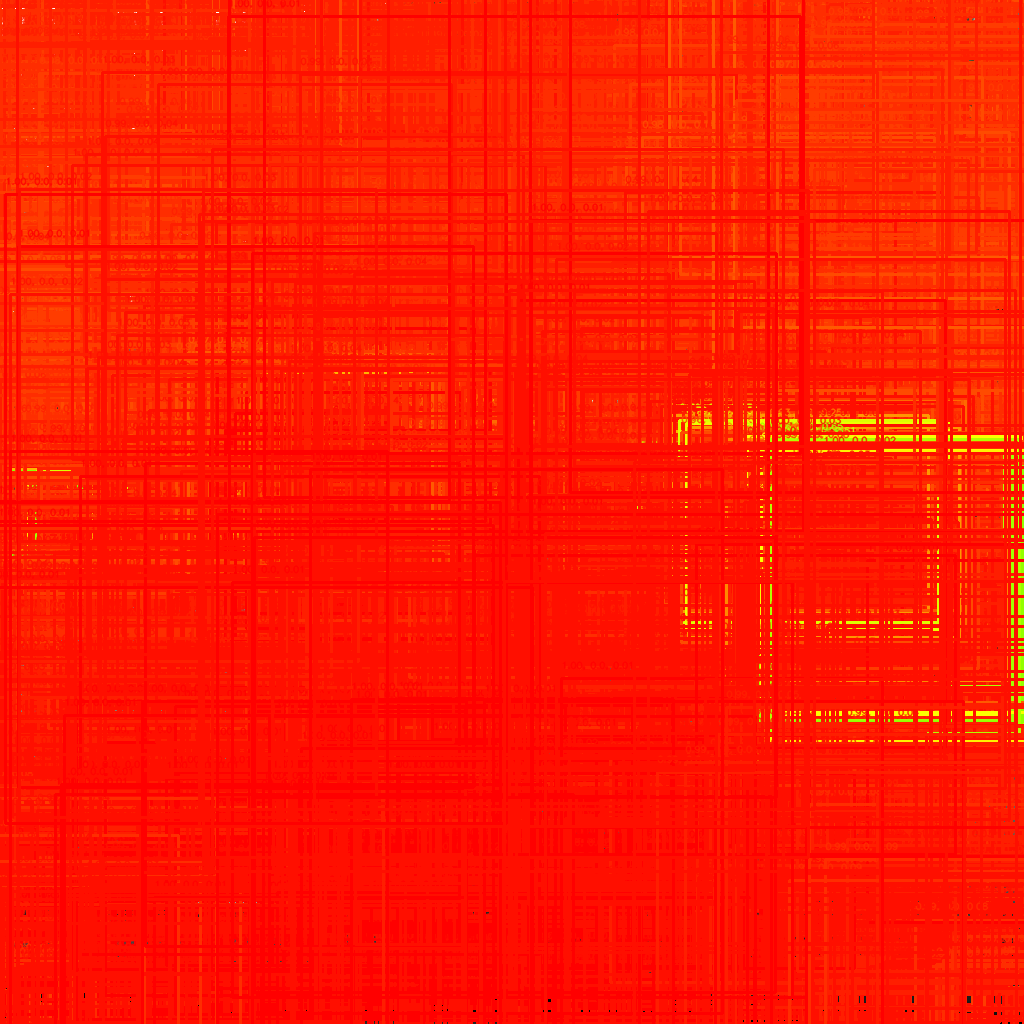
\includegraphics[width=\textwidth]{images/uq_weathers/SubEns_entropies_all2.png}
            \end{column}
            \begin{column}{.2\textwidth}
                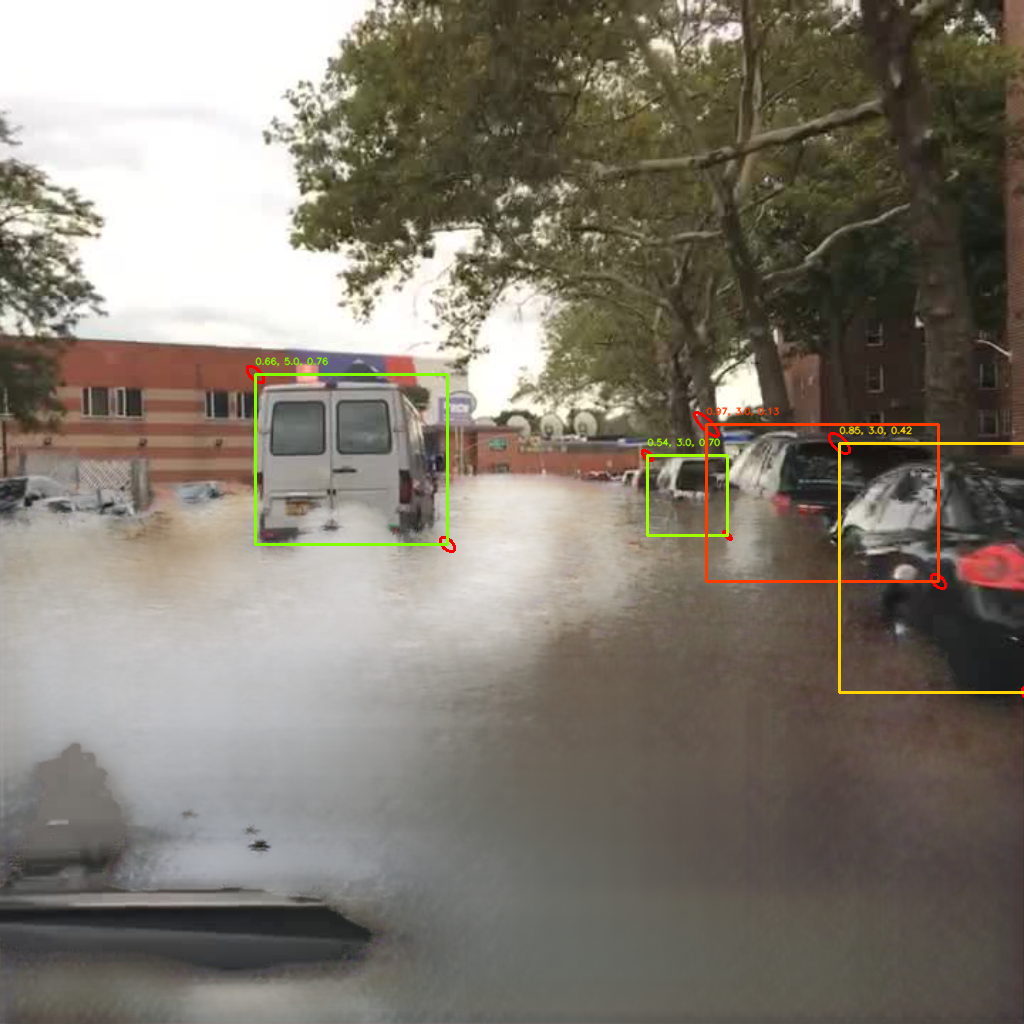
\includegraphics[width=\textwidth]{images/uq_weathers/SubEns_Variance1.png}
                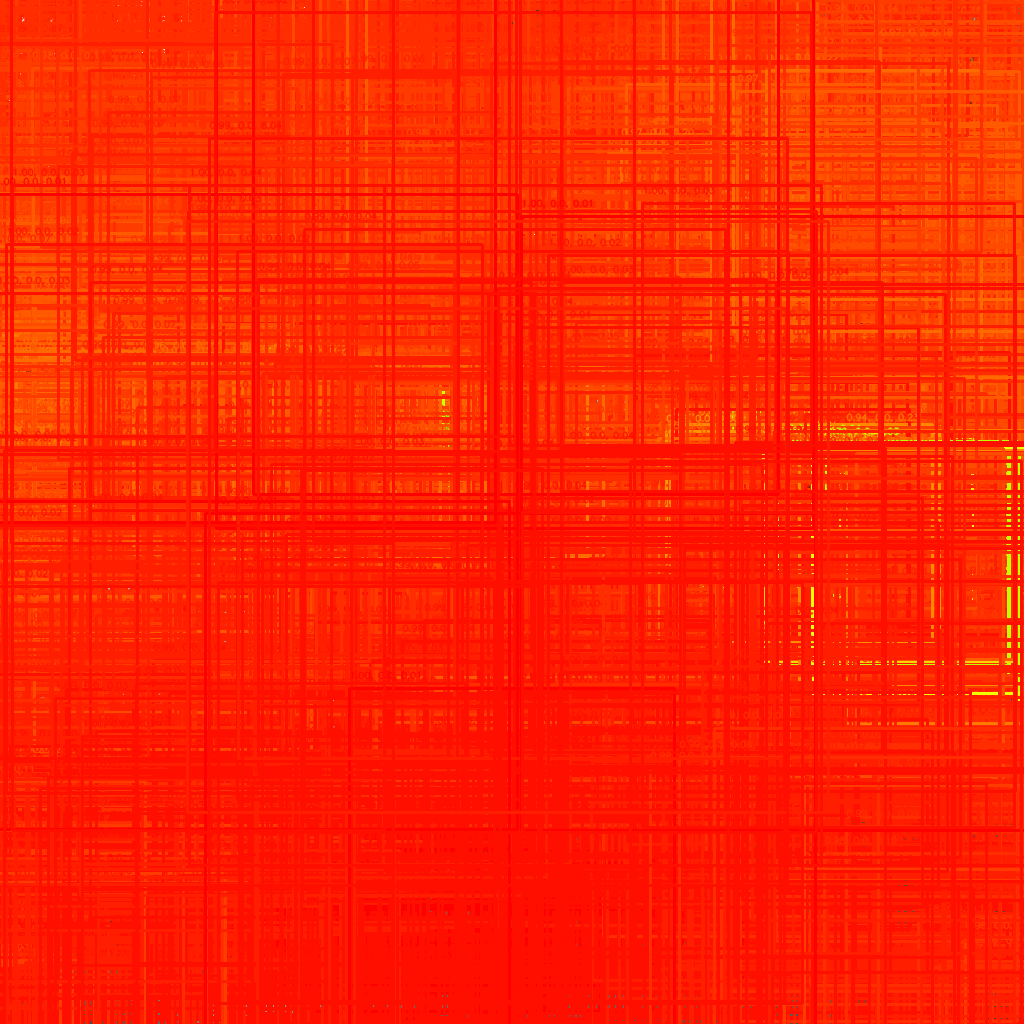
\includegraphics[width=\textwidth]{images/uq_weathers/SubEns_entropies_all1.png}
            \end{column}
            \begin{column}{.2\textwidth}
                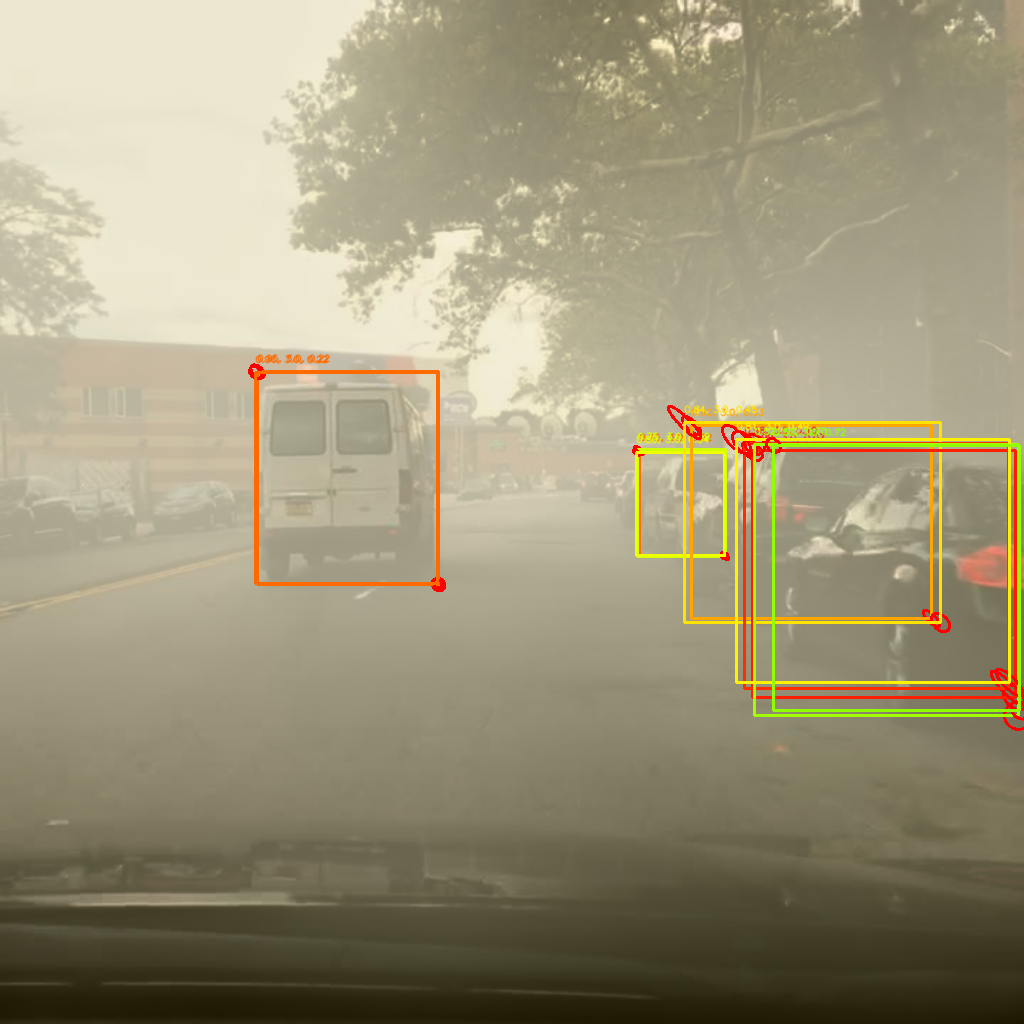
\includegraphics[width=\textwidth]{images/uq_weathers/SubEns_Variance3.png}
                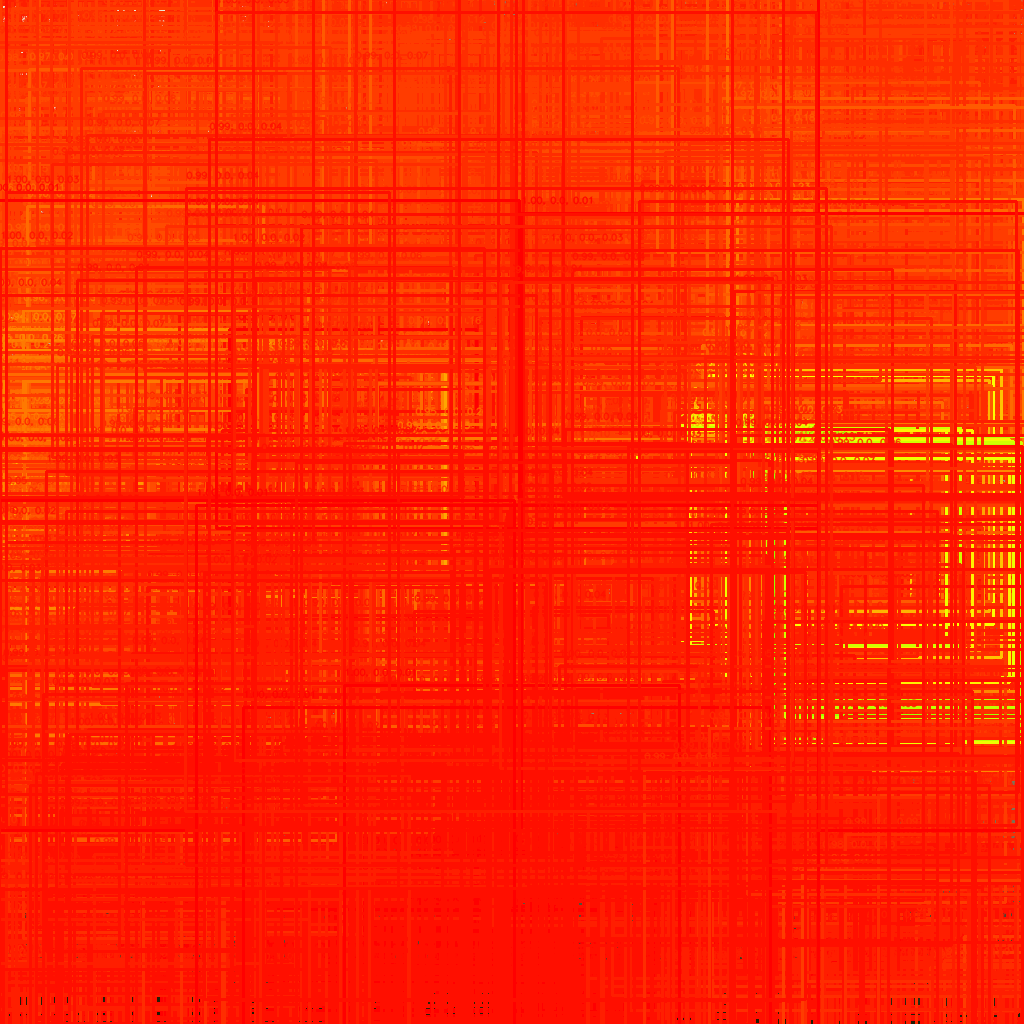
\includegraphics[width=\textwidth]{images/uq_weathers/SubEns_entropies_all3.png}
            \end{column}
            \begin{column}{.2\textwidth}
                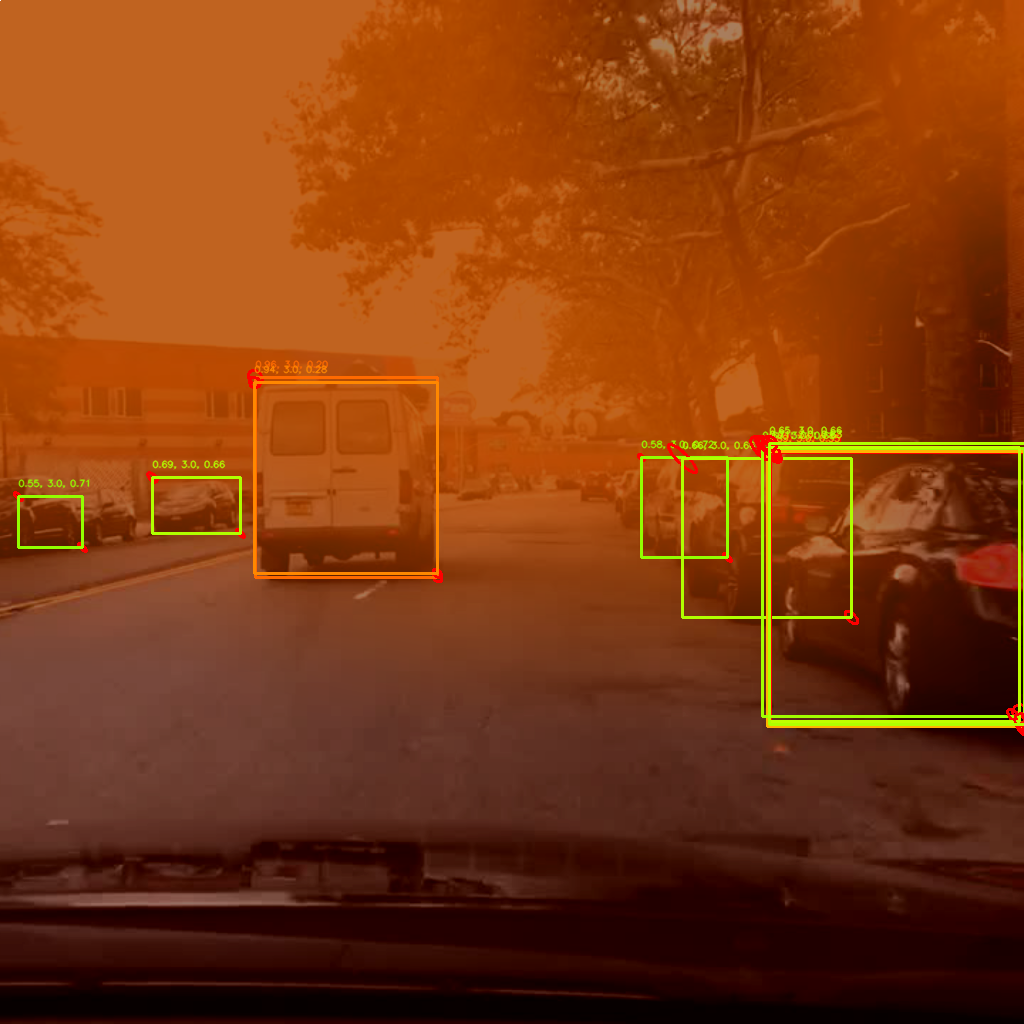
\includegraphics[width=\textwidth]{images/uq_weathers/SubEns_Variance4.png}
                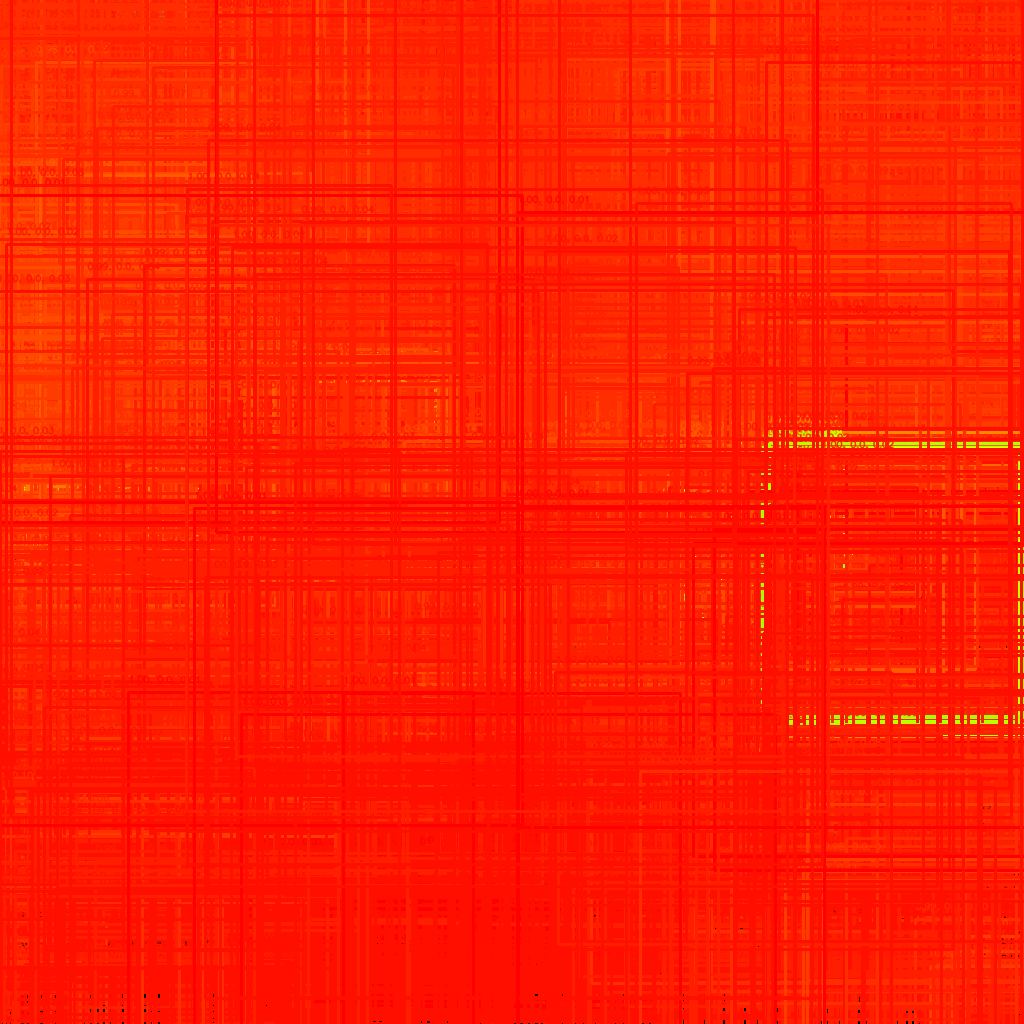
\includegraphics[width=\textwidth]{images/uq_weathers/SubEns_entropies_all4.png}
            \end{column}
        \end{columns}
        \begin{center}
            Performance of Sub-Ensembles on BDD100K weather dataset
        \end{center}
      

        % \begin{figure}
        %     \centering
        %     \begin{minipage}{.225\textwidth}
        %     \centering
        %     \includegraphics[width=\linewidth]{images/uq_weathers/sub}
        %     \caption{A subfigure}
        %     \end{minipage}
        %     \begin{minipage}{.225\textwidth}
        %     \centering
        %     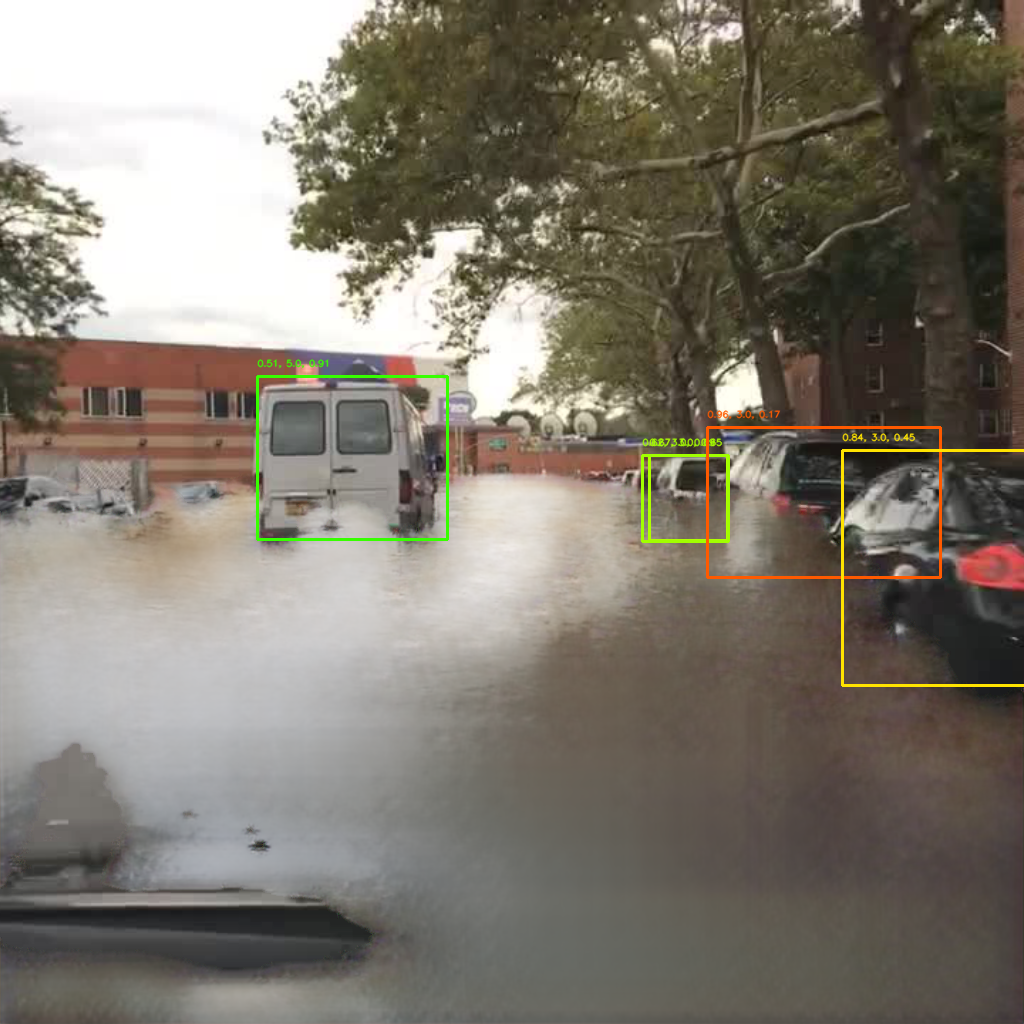
\includegraphics[width=\linewidth]{images/uq_weathers/BNN_entropies1.png}
        %     \caption{A subfigure}
        %     \end{minipage}
        %     \begin{minipage}{.225\textwidth}
        %         \centering
        %         \includegraphics[width=\linewidth]{images/uq_weathers/BNN_entropies3.png}
        %         \caption{A subfigure}
        %     \end{minipage}
        %     \begin{minipage}{.225\textwidth}
        %         \centering
        %         \includegraphics[width=\linewidth]{images/uq_weathers/BNN_entropies4.png}
        %         \caption{A subfigure}
        %     \end{minipage}
        %     \caption{A figure with two subfigures}
        % \end{figure}

        % \begin{figure}[ht]
        %     \captionsetup[subfigure]{labelformat=empty}
        %     \begin{tabular}{cccc}
        %         \subfloat{\includegraphics[width = 1.4in]{images/uq_weathers/BNN_entropies2.png}} &
        %         \subfloat{\includegraphics[width = 1.4in]{images/uq_weathers/BNN_entropies1.png}} &
        %         \subfloat{\includegraphics[width = 1.4in]{images/uq_weathers/BNN_entropies3.png}} &
        %         \subfloat{\includegraphics[width = 1.4in]{images/uq_weathers/BNN_entropies4.png}}\\
        %         \subfloat{\includegraphics[width = 1.4in]{images/uq_weathers/BNN_variances2.png}} &
        %         \subfloat{\includegraphics[width = 1.4in]{images/uq_weathers/BNN_variances1.png}} &
        %         \subfloat{\includegraphics[width = 1.4in]{images/uq_weathers/BNN_variances3.png}} &
        %         \subfloat{\includegraphics[width = 1.4in]{images/uq_weathers/BNN_variances4.png}}\\
        %         \subfloat[Normal Weather]{\includegraphics[width = 1.4in]{images/uq_weathers/flipout_entropies_all2.png}} &
        %         \subfloat[Flood]{\includegraphics[width = 1.4in]{images/uq_weathers/flipout_entropies_all1.png}} &
        %         \subfloat[Smog]{\includegraphics[width = 1.4in]{images/uq_weathers/flipout_entropies_all3.png}} &
        %         \subfloat[Wild Fire]{\includegraphics[width = 1.4in]{images/uq_weathers/flipout_entropies_all4.png}}\\
        %     \end{tabular}
        %     \caption[Detection on an image from \acrshort{bdd-c} dataset using \acrshort{bnn}]{Detection and entropy visualization on a randomly sampled image from the \acrshort{bdd-c} dataset using \acrshort{bnn}. We can observe that the model struggled in detecting objects as weather intensity increases. Also we can observe that there are lot less detection boxes seen compared to un-changed input image. The all boxes figure shows that majority of the boxes belong to background}
        %     \label{Flipout_uq_det}
        % \end{figure}
\pagebreak
\begin{columns}
    \column{0.45\linewidth}
    \begin{table}[H]
        \centering
        \footnotesize
        \caption{Uncertainty quantification metrics calculated using Bayesian and Sub-Ensemble versions of SSD300 model}
        \label{tab:my-table}
        \begin{tabular}{llll}
            \hline
                      &               & \begin{tabular}[c]{@{}l@{}}Bayesian\\ SSD300\end{tabular} & \begin{tabular}[c]{@{}l@{}}Sub-Ensemble\\ SSD300\end{tabular} \\ \hline
            Flood     & Probability   & 0.43            & 0.5                                                           \\ \hline
                      & Entropy       & \textbf{0.57}            & 0.5                                                           \\ \hline
                      & Box Deviation & 0.46            & 0.5                                                           \\ \hline
            Smog      & Probability   & 0.43            & 0.5                                                           \\ \hline
                      & Entropy       & \textbf{0.57}            & 0.5                                                           \\ \hline
                      & Box Deviation & 0.44            & 0.5                                                           \\ \hline
            Wild Fire & Probability   & \textbf{0.51}            & \textbf{0.53}                                                          \\ \hline
                      & Entropy       & 0.49            & 0.46                                                          \\ \hline
                      & Box Deviation & 0.49            & 0.46                                                          \\ \hline
        \end{tabular}
    \end{table}
    \column{0.45\linewidth}
        \begin{itemize}
            \item change in weather the object detection performance has deteriorated especially
            in the case of flood images.
            \item scores suggest that using uncertainty quantification methods performed almost similar
            to an unbiased random classifier.
            \item uncertainty quantification methods not being able to detect skewed datasets
            complies with the results reported by \citet{Ovadia2019}
        \end{itemize}
\end{columns}
\end{frame}

\section{Contributions}
\begin{frame}[allowframebreaks]{Contributions}
    \begin{itemize}
        \item Proposed a new benchmark dataset called Out-of-Distribution detection for Object Detection ($OD^2$) dataset
        \item Max Softmax, ODIN, Mahalanobis distance based OOD detector, and uncertainty based OOD detector are modelled.
        \item Single Shot multi-box Object Detector (SSD300) is trained on BDD100K dataset and tuned the prior boxes
        \item we observed that ODIN outperformed the Max-Softmax based OOD detectors, could not successfully model Mahalanobis distance-based OOD detector.
        \item BNN based and a Sub-Ensemble model of SSD object detector network are modelled and trained.
        \pagebreak
        \item We used entropy to quantify uncertainty in the classification head of object detector and box deviation to quantify uncertainty in the regression head of object detectors.
        \item We performed extensive experimentation on all the three available OOD detectors for object detection purposes. We also performed studies on the class-specific behavior of the uncertainty quantification metrics.
    \end{itemize}
\end{frame}

\section{Observations}
\begin{frame}[allowframebreaks]{Observations}
    \begin{itemize}
        \item object detector performance is dependent on the prior knowledge of the dataset. 
        \item Deep learning-based object detectors struggle when deployed in open environments.
        \item The OOD detection methods proposed for classification did not directly transfer their performance into the task of object detection.
        \item Sub-Ensemble-based uncertainty quantification with box deviation as a metric out-performed all other methods in OOD detection.
        \item Entropy struggled in detecting samples that are ambiguous due to their semantic appearance.
        \item The OOD detection methods proposed in this work did not work as expected on the BDD100K-Weather data in the $OD^2$ benchmarking dataset.
    \end{itemize}
\end{frame}

\section{Future-work}
\begin{frame}[allowframebreaks]{Future-work}
    \begin{itemize}
        \item An object detector without the usage of background class would be useful for improved OOD performance.
        \item Exploring the effects of uncertainty calibration methods \cite{GuoCalibration2017} on OOD detection is still a open-ended question.
        \item combining Entropy and Box-Deviation to obtain a single novelty score might result in a better representation of OOD detection ability.
        \item Disentangling of Predictive uncertainty.
        \item Though we believe a strong benchmark in the form of $OD^2$ dataset is proposed, we believe it can be further modified and extended to include more class-agnostic tasks.
    \end{itemize}
\end{frame}

\begin{frame}[allowframebreaks]
    \frametitle{References}
    \bibliographystyle{unsrtnat}
    % \bibliography{bibliography.bib}
    {\small
\bibliography{bibliography.bib}}
\end{frame}
\end{document}
